%% fleqn -> alle Formeln linksb�ndig
%% oneside -> einseitig, wichtig f�r Kopf- und Fusszeilen
%% smallheadings -> �berschriften sind nicht riesen gro�, sondern ca. 2 gr��er als section-�berschriften
%\documentclass[listof=totoc,12pt,a4paper,twoside,idxtotoc,normalheadings,bibtotoc]{scrreprt}
\documentclass[listof=totoc,12pt,a4paper,twoside,idxtotoc,normalheadings,bibtotoc,open=left]{scrbook}
\listfiles


%%%%%%%%%%%%%%%%%%%%%%%%%%
%% Formate f�r die Seitendarstellung der gesamten Arbeit
%%%%%%%%%%%%%%%%%%%%%%%%%%

%% Anpassen des Seitenlayouts
\usepackage{geometry}
%% nach HTW-Layoutanforderung
\geometry{verbose,a4paper,tmargin=3cm,bmargin=3cm,lmargin=35mm,rmargin=2cm}
%% Um z.B. eine Seite im Querformat darzustellen
\usepackage{lscape}
%% leere letzte Seite
\usepackage{lastpage}
%% Elemente auch fest positionieren 
\usepackage{float}
\usepackage{floatflt}
\usepackage{wrapfig} % Alternative zu floatflt
\usepackage{picins} % Alternative zu floatflt und wrapfig
%\usepackage{nonfloat}
%% Befehl, damit alle Float-Elemente bis zu dem Punkt positioniert werden -> \FloatBarrier
\usepackage{placeins}

%% Abstand zwischen Abschnitten und Zeilen
\setlength{\parindent}{0ex} %% Einzug erste Zeile neues Kapitel bzw. Absatz
\setlength{\parskip}{2.0ex plus 0.9ex minus 0.4ex} %% L�cke zwischen 2 Abs�tzen
%% Zeilenabstand
% Variante 1 -> linespread
%\linespread{1.3} %% 1,3*1,2 = 1,56fach ---> vielleicht am Besten!
% Variante 2 -> onehalfspacing
\usepackage{setspace}
\onehalfspacing




%% Hurenkinder / Schusterjungen
\clubpenalty = 10000
\widowpenalty = 10000 \displaywidowpenalty = 10000

%Sorgt beim Dokumenttyp book daf�r, da� kein Ausgleich des unteren Seitenrandes durch Dehnung der Absatzabst�nde durchgef�hrt wird. \raggedbottom ist bei den Dokumenttypen article, report und letter bereits voreingestellt. 
\raggedbottom


%%%%%%%%%%%%%%%%%%%%%%%%%%
%% Tabellen
%%%%%%%%%%%%%%%%%%%%%%%%%%

%% �berlange Tabellen
% http://www.ctan.org/tex-archive/macros/latex/contrib/xcolor/
\usepackage[table]{xcolor}
\usepackage{longtable}
\usepackage{array}

%% Mehrere Zeilen zusammenfassen
\usepackage{multirow}
%% Farbige Tabellenzellen
\usepackage{colortab}
\usepackage{colortbl}


%%%%%%%%%%%%%%%%%%%%%%%%%%
%% Schriftarten
%%%%%%%%%%%%%%%%%%%%%%%%%%

%% Zeilenabstand
\renewcommand{\baselinestretch}{1.2}\normalsize

%% Use T1-fontencoding, u.a. um Schrift auf Bildschirm gut anzuzeigen
\usepackage[T1]{fontenc}  % T1-Font
%% Latin1 Codepage, u.a. f�r Umlaute
%\usepackage[latin1]{inputenc}  % Latin
\usepackage[ansinew]{inputenc}  % ANSI
% Damit erscheinen Umlaute auch wirklich als Umlaute im PDF
\usepackage{ae}
%% A package to use PostScript Times Roman as the default font.
%%\usepackage{times}\usepackage{mathptmx}
%% Verbatim-Umgebung
%\usepackage{verbatim}
%% Einbinden der Ding-Sonderzeichen
\usepackage{pifont}
\usepackage{textcomp}
%% Sonderzeichen & Mathe
\usepackage{amsmath}
\usepackage{amsfonts}
\usepackage{amssymb}
\usepackage{wasysym} 
%%\usepackage{marvosym}
%% Euro-Zeichen
\usepackage{eurosym}
%% Anderer Pfeil f�r Listen
\renewcommand{\labelitemi}{\ding{226}}

%% Erweiterung der Listen
\usepackage{enumitem}
\usepackage{expdlist}

\newcommand{\pro}{\ensuremath{+}}
\newcommand{\contra}{\ensuremath{-}}
\newcommand{\procon}{\ensuremath{+-}}
%\renewcommand{\labelitemii}{\ding{218}}

%\setlength{\labelsep}{5cm}



%%%%%%%%%%%%%%%%%%%%%%%%%%
%% Regionale Anpassungen
%%%%%%%%%%%%%%%%%%%%%%%%%%

%% f�r deutsche Silbentrennung
%\usepackage{ngerman}
%% Multilanguage Support for LaTeX, oder hier mit Umlauten...
\usepackage[ngerman]{babel}
%% Anf�hrungszeichen
%% sorgt daf�r, da� es einheitlich ist
\usepackage[babel,german=quotes]{csquotes}
\usepackage[ngerman]{translator}

%\usepackage[babel,german=quotes]{csquotes} % Deutsche
%\usepackage[babel,german=swiss]{csquotes} % Schweizer
%\usepackage[babel,german=guillemets]{csquotes} % Franz�sische
%\usepackage[babel,english=american]{csquotes} % Amerikanische
%\usepackage[babel,english=british]{csquotes} % Englische
%Demo Hallo \enquote{World}!



%%%%%%%%%%%%%%%%%%%%%%%%%%
%% Inhaltsverzeichnis, Titelseite
%%%%%%%%%%%%%%%%%%%%%%%%%%

%% zum Ver�ndern der Verzeichnisse Inhalt, Abbildung, Tabellen
\usepackage{titletoc}

%% Index, TableOfContents und TheBibliography mit ins Inhaltsverzeichnis aufnehmen
%\usepackage[nottoc]{tocbibind}

%% Im Inhaltsverzeichnis zwei Ebenen tiefer anzeigen, z.B. 3.4.1.1 erm�glichen
% von \chapter an 3 Ebenen tiefer
\setcounter{tocdepth}{4}
\setcounter{secnumdepth}{4}




%%%%%%%%%%%%%%%%%%%%%%%%%%
%% Abk�rzungsverzeichnis
%%%%%%%%%%%%%%%%%%%%%%%%%%
%\usepackage[intoc,german]{nomencl}
%% Umbenennen
%\renewcommand{\nomname}{Abk\"urzungsverzeichnis}

%\let\abk\nomenclature
%\setlength{\nomlabelwidth}{.20\hsize}
%\renewcommand{\nomlabel}[1]{#1 \dotfill}
%\setlength{\nomitemsep}{-\parsep}
%\makenomenclature


%%%%%%%%%%%%%%%%%%%%%%%%%%
%% Glossar
%%%%%%%%%%%%%%%%%%%%%%%%%%

%% Glossary f�r Glossare (veraltet)
%\usepackage[cols=3,toc=true,header=plain,style=super]{glossary}
%\renewcommand{\glossaryname}{Glossar}
%\renewcommand{\entryname}{Begriff}
%\renewcommand{\descriptionname}{Beschreibung}
%\makeglossary

\usepackage[
toc,
nonumberlist, %keine Seitenzahlen anzeigen
acronym,      %ein Abk�rzungsverzeichnis erstellen
toc,          %Eintr�ge im Inhaltsverzeichnis
section]      %im Inhaltsverzeichnis auf section-Ebene erscheinen
{glossaries}


%Den Punkt am Ende jeder Beschreibung deaktivieren
\renewcommand*{\glspostdescription}{}



%Glossar-Befehle anschalten
\makeglossaries

%Diese Befehle sortieren die Eintr�ge in den
%einzelnen Listen:
%makeindex -s datei.ist -t datei.alg -o datei.acr datei.acn
%makeindex -s datei.ist -t datei.glg -o datei.gls datei.glo
%makeindex -s datei.ist -t datei.slg -o datei.syi datei.syg



%%%%%%%%%%%%%%%%%%%%%%%%%%
%% Index
%%%%%%%%%%%%%%%%%%%%%%%%%%

%% .idx-Datei erstellen f�r Sachregister
\usepackage{makeidx}

%% Aufforderung zum Suchen der Index-Begriffe
\makeindex
%% Umbenennung von Index zu Stichwortverzeichnis (u.a. wichtig f�r Seitentitel)
\renewcommand{\indexname}{Stichwortverzeichnis}
% einzelne Seite kursiv und fett, neue Befehle: idxbf / idxit
\newcommand{\idxit}[1]{{\it #1}} 
%% \newcommand{\idxit}[1]{\it{#1}} - funkt nicht sauber
\newcommand{\idxbf}[1]{{\bf #1}}
% anstelle siehe, nur s.
\renewcommand{\seename}{s.}



%%%%%%%%%%%%%%%%%%%%%%%%%%
%% Fu�noten
%%%%%%%%%%%%%%%%%%%%%%%%%%

%% Speichern von Fu�notennummern
\usepackage{savefnmark}

%%%%%%%%%%%%%%%%%%%%%%%%%%
%% Zitate / Literaturverzeichnis
%%%%%%%%%%%%%%%%%%%%%%%%%%

% Festlegung Art der Zitierung - Havardmethode: Abkuerzung Autor + Jahr
%\bibliographystyle{alphadin}
% fuer Zitate
%\usepackage[round]{natbib}
%\bibpunct{[}{]}{;}{}{}{,}

%% Biblatex
\usepackage[backend=biber,style=alphabetic-verb]{biblatex} %Zitierpacket laden, Stil l�sst sich �ber "style" bestimmen

\bibliography{verzeichniss}
	
	
%Alle B�cher werden eingebunden
%\nocite{*}



%%%%%%%%%%%%%%%%%%%%%%%%%%
%% Listings (Code) nativ darstellen
%%%%%%%%%%%%%%%%%%%%%%%%%%

\usepackage{listings}

\lstloadlanguages{[Sharp]C}






\renewcommand{\lstlistlistingname}{Auflistungen}

%%%%%%%%%%%%%%%%%%%%%%%%%%%
%%%%%%%%%%%%%%%%%%%%%%%%%%%%
\usepackage[font=small,labelfont=bf,format=hang]{caption}
% ,justification=RaggedRight -> geht ni
%% sp�ter �nderbar mit \captionsetup
%% �berschrift f�r Tabellen, funktioniert aber nicht,
%% darum \caption vor \tabular f�r jede Tabelle einzeln
\captionsetup[table]{position=above,belowskip=5pt,aboveskip=5pt}
\captionsetup[figure]{position=below,belowskip=5pt,aboveskip=5pt}
\usepackage{tabularx}





%%%%%%%%%%%%%%%%%%%%%%%%%%
%% Kopf- und Fusszeilen
%%%%%%%%%%%%%%%%%%%%%%%%%%

%% Kopf- und Fusszeilen mit KOMA
\usepackage[automark,headsepline,nouppercase]{scrpage2}
%% Abstand der Kapitel�berschrift von der Kopfzeile
\renewcommand*{\chapterheadstartvskip}{\vspace*{-\topskip}}
%% auch bei Kapitel�berschriften Kopfzeile anwenden
\renewcommand*{\chapterpagestyle}{scrheadings}
\renewcommand*{\indexpagestyle}{scrheadings}

%%%%%%%%%%%%%%%%%%%%%%%%%%%%
%% Kopfzeilen anpassen (package scrpage2)
%%%%%%%%%%%%%%%%%%%%%%%%%%

%% KOMA-Skript Kopfzeilen auf den Seiten
\pagestyle{scrheadings}
%% automatisch Kapitel�berschriften (Kolumnentitel) in Kopfzeile aktualisieren
\automark[section]{chapter}
%% alle Felder beider Seitenstile auf leere Inhalte setzen
\clearscrheadfoot
%% linke Kopfzeile (bei 2seitig --> Book)
\rohead{\headmark}{\headmark}
%% rechte Kopfzeile - �berschrift ausgeben
\lehead[\headmark]{\headmark}
%durch Angabe des optionalen Parameters �ndert man scrplain mit!
%% rechte Fusszeile - Seitenzahl (\thepage)
\ofoot[\pagemark]{\pagemark}
%% Kopfzeilentext + Linie: Verschiebung vom linken Rand weg, Breite der Kopfzeile
\setheadwidth[0pt]{text}
%% St�rke der Trennlinie zum Text
\setheadsepline{.4pt}
%% Schriftgr��e der Kopfzeile kleiner machen (10) -> bringt Warnung
\setkomafont{pagehead}{\small}
%\setkomafont{pagefoot}{\normalsize}




%%%%%%%%%%%%%%%%%%%%%%%%%%%%
%% �berschriften formatieren
%%%%%%%%%%%%%%%%%%%%%%%%%%%%

\renewcommand*{\theparagraph}{\thesubsubsection.\arabic{paragraph}}

\usepackage[clearempty]{titlesec} % wei� nicht, was clearempty macht
  \titleformat{\chapter}%
    {\normalfont\Large\bfseries}% \Large sollte Gr��e 16 sein, relativ zu Normal (12)
    {\thechapter}%
    {1em}% Abstand Nummerierung zum �berschriftstext
    {}%
    %% Chapter-�berschrift ein St�ck weiter unten als Section-�berschriften oder 
    %% restlicher Text --> 2. Klammernpaar
    %\titlespacing{\chaptaer}{0pt}{*0}{*5}
    \titlespacing{\chapter}{0pt}{-1.5em}{*5}
    %% {Einzug (Abstand zum linken Rand)} / 
    %% {Abstand zur Kopfzeile als Multiplikator zu ? bzw. als explizite Angabe} / 
    %% {Abstand �berschrift zum folgenden Text}
  \titleformat{\section}%
    {\normalfont\large\bfseries}% \large sollte Gr��e 14 sein
    {\thesection}%
    {1em}%
    {}%
  \titleformat{\subsection}%
    {\normalfont\normalsize\bfseries}%
    {\thesubsection}%
    {1em}%
    {}%
	\titleformat{\subsubsection}%
    {\normalfont\small\bfseries}%
    {\thesubsubsection}%
    {1em}%
    {}%
  \titleformat{\paragraph}% ohne [runin] steht paragraph-Text extra mit Leerzeile
  	%% zum Folgetext
    {\normalfont\small\itshape}%
    {\theparagraph}%
    {1em}%
    {}%


%%%%%%%%%%%%%%%%%%%%%%%%%%%%
%% PDF-Generierung
%%%%%%%%%%%%%%%%%%%%%%%%%%%%

\usepackage{pdfpages}
\usepackage{pst-pdf}
\usepackage{pstricks, pst-node, pst-plot, pst-math, pst-optic, pst-lens, pst-text, pst-xkey, pstricks-add}
\usepackage{ifpdf}
\ifpdf
%		\usepackage[pdftex]{graphicx}
%		\DeclareGraphicsExtensions{.eps,.jpg,.png,.pdf}
		\usepackage[
			pdftex=true
			,hyperfigures=true
			,backref=false
			,hyperindex=true
			,bookmarksnumbered=true
			,bookmarksopen=true
			,colorlinks=true
			,citecolor=black
			,linkcolor=black
			,urlcolor=black
			,filecolor=magenta
			,pdfborder={0 0 0}
			,pdfstartview=FitH
			,plainpages=false
			]{hyperref}
		\pdfinfo{
			/Title (Diplomarbeit)
			/Subject (Titel)
			/Author (Martin Domnick)
			/Keywords ()
		}		
		\else
%			\usepackage[dvips]{graphicx}
%			\DeclareGraphicsExtensions{.png,.eps,.gz}
			\usepackage[
				hypertex=true
				,hyperref=true
				%,hyperfigures=true
				,backref=true
				,hyperindex=true
				,bookmarksnumbered=true
				,colorlinks=true
				,linkcolor=blue
				,urlcolor=blue
				,filecolor=magenta
				,german
			]{hyperref}
\fi

%% Gesataltung von Hyperlinks
%\package{url}
\urlstyle{same}

\def\UrlFont{\em}


%%%%%%%%%%%%%%%%%%%%%%%%%%%%
%% Sonstige Klassen
%%%%%%%%%%%%%%%%%%%%%%%%%%%%

%% Befehle wiederholbar
\usepackage{multido}
%% Drehung von einzelnen Objekten
\usepackage{rotating}


%% ????
\makeatletter
  \renewenvironment{itemize}{\begin{list}{\csname\itemitem\endcsname}{
 \advance\@itemdepth 1 \edef\itemitem{labelitem\romannumeral\the\@itemdepth}
 \labelwidth 1em \itemindent 0em \leftmargin 2em \rightmargin 1em
 \parsep 0pt \itemsep 1pt plus 0.5pt minus 0.5pt
 \topsep 0pt minus 3.5pt \partopsep 0pt  minus 1.5pt}}{\end{list}} 
\makeatother 



%%%%%%%%%%%%%%%%%%%%%%%%%%%%
%% Spezielle Erg�nzungen f�r PS
%%%%%%%%%%%%%%%%%%%%%%%%%%%%

%% Farben f�r PSforPDF definieren
\usepackage{color}


\definecolor{hellgrau}{gray}{0.85}
\definecolor{dunkelgrau}{gray}{0.4}
\definecolor{orange}{rgb}{1.,0.65,0}
\definecolor{dunkelgruen}{rgb}{0,0.5,0}
\definecolor{dunkelblau}{rgb}{0,0,0.5}
\definecolor{dunkelrot}{rgb}{0.5,0.0,0.0}
\definecolor{hellrot}{rgb}{1.0,0.5,0.5}
\definecolor{hellblau}{rgb}{0.25,0.25,1}
\definecolor{hellgruen}{rgb}{0.25,1,0.25}
\definecolor{schwarz}{rgb}{0,0,0}
%%%%%%%%%%%%%%%%%%%%%%%%%%%%
%% Eigene Boxen definieren
%%%%%%%%%%%%%%%%%%%%%%%%%%%%



%% Eigenen Boxtyp Box definiert
\makeatletter
\def\RPBox{\pst@object{RPBox}}
\def\RPBox@i#1#2#3{{%
\use@par                        % Local parameters
\if@star\solid@star\fi          % Stared version
\pssetlength{\pst@dimc}{-\psframesep}
\psaddtolength{\pst@dimc}{-\psframesep}
\psaddtolength{\pst@dimc}{-\pslinewidth}
\psaddtolength{\pst@dimc}{-\pslinewidth}
\pssetlength{\pst@dima}{#1}
\psaddtolength{\pst@dima}{\pst@dimc}
\pssetlength{\pst@dimb}{#2}
\psaddtolength{\pst@dimb}{\pst@dimc}
\setbox\z@\vbox to\pst@dimb{\hsize\pst@dima\sloppy\vfil\scriptsize{\begin{center}#3\end{center}}\vfil}%
%\psset{shadow=true}\psframebox{\box\z@}\psset{shadow=false}}}
\psframebox{\box\z@}}}
\makeatother

%% Eigenen Boxtyp Box definiert
\makeatletter
\def\RPBoxB{\pst@object{RPBoxB}}
\def\RPBoxB@i#1#2#3{{%
\use@par                        % Local parameters
\if@star\solid@star\fi          % Stared version
\pssetlength{\pst@dimc}{-\psframesep}
\psaddtolength{\pst@dimc}{-\psframesep}
\psaddtolength{\pst@dimc}{-\pslinewidth}
\psaddtolength{\pst@dimc}{-\pslinewidth}
\pssetlength{\pst@dima}{#1}
\psaddtolength{\pst@dima}{\pst@dimc}
\pssetlength{\pst@dimb}{#2}
\psaddtolength{\pst@dimb}{\pst@dimc}
\setbox\z@\vbox to\pst@dimb{\hsize\pst@dima\sloppy\vfil\scriptsize{\begin{center}#3\end{center}}\vfil}%
\psset{shadow=true}\psframebox{\box\z@}\psset{shadow=false}}}
%\psframebox{\box\z@}}}
\makeatother



%% Eigenen Boxtyp DiaBox definiert
\makeatletter
\def\RPDiaBox{\pst@object{RPDiaBox}}
\def\RPDiaBox@i#1#2#3{{%
\use@par                        % Local parameters
\if@star\solid@star\fi          % Stared version
\pssetlength{\pst@dimc}{-\psframesep}
\psaddtolength{\pst@dimc}{-\psframesep}
\psaddtolength{\pst@dimc}{-\pslinewidth}
\psaddtolength{\pst@dimc}{-\pslinewidth}
\pssetlength{\pst@dima}{#1}
\psaddtolength{\pst@dima}{\pst@dimc}
\pssetlength{\pst@dimb}{#2}
\psaddtolength{\pst@dimb}{\pst@dimc}
\setbox\z@\vbox to\pst@dimb{\hsize\pst@dima\sloppy\vfil\scriptsize{\begin{center}#3\end{center}}\vfil}%
\psdiabox{\box\z@}}}
\makeatother

%% Eigenen Boxtyp Fpnfeck definiert
\makeatletter
\def\PSPentBox{\pst@object{PSPentBox}}
\def\PSPentBox@i#1#2{{%
\use@par                        % Local parameters
\if@star\solid@star\fi          % Stared version
\pssetlength{\pst@dimc}{-\psframesep}
\psaddtolength{\pst@dimc}{-\psframesep}
\psaddtolength{\pst@dimc}{-\pslinewidth}
\psaddtolength{\pst@dimc}{-\pslinewidth}
\pssetlength{\pst@dima}{#1}
\psaddtolength{\pst@dima}{\pst@dimc}
\pssetlength{\pst@dimb}{#1}
\psaddtolength{\pst@dimb}{\pst@dimc}
\setbox\z@\vbox to\pst@dimb{\hsize\pst@dima\sloppy\vfil\scriptsize{\begin{center}#2\end{center}}\vfil}%
\pscustom{
	\psline(0.79385\pst@dima,0.0955\pst@dima)
				(0.20615\pst@dima,0.0955\pst@dima)
				(0.02445\pst@dima,0.6545\pst@dima)
				(0.5\pst@dima,\pst@dima)%
				(0.97555\pst@dima,0.6545\pst@dima)
				(0.79385\pst@dima,0.0955\pst@dima)
				(0.20615\pst@dima,0.0955\pst@dima)
}{\box\z@}a
}}
\makeatother


%% Abk�rzungsverzeicnis - Punkte

%\makeatletter% --> De-TeX-FAQ
%\renewcommand*{\lstlistoflistings}{%
%  \begingroup
%    \if@twocolumn
%      \@restonecoltrue\onecolumn
%    \else
%      \@restonecolfalse
%    \fi
%    \lol@heading
%    \setlength{\parskip}{\z@}%
%    \setlength{\parindent}{\z@}%
%    \setlength{\parfillskip}{\z@ \@plus 1fil}%
%    \@starttoc{lol}%
%    \if@restonecol\twocolumn\fi
%  \endgroup
%}
%\makeatother% --> \makeatletter


%\newcommand{\kommentar}[1]{}


%%%%%%%%%%%%%%%%%%%%%%%%%%%%
%% Silbentrennung
%%%%%%%%%%%%%%%%%%%%%%%%%%%%

%\hyphenation{End-an-wen-der}

\setkomafont{sectioning}{\normalfont\bfseries}
\setkomafont{captionlabel}{\normalfont\bfseries}
\setkomafont{pagehead}{\normalfont\itshape}
\setkomafont{descriptionlabel}{\normalfont\bfseries}


%%%%%%%%%%%%%%%%%%%%%%%%%%%%
%% Bilder
%%%%%%%%%%%%%%%%%%%%%%%%%%%%

\usepackage{graphicx}

%%%%%%%%%%%%%%%%%%%%%%%%%%%%
%% Anhang
%%%%%%%%%%%%%%%%%%%%%%%%%%%%
\usepackage{appendix}
%\renewcommand\appendix{\par
%  \setcounter{chapter}{0}%
%  \setcounter{section}{0}%
%  \gdef\@chapapp{\appendixname}%
%  \gdef\thechapter{\@Alph\c@chapter}}

%% Quellcode

%% Copyrights, Marken, etc...

\def\TReg{\textsuperscript{\textregistered}}
\def\TCop{\textsuperscript{\textcopyright}}
\def\TTra{\textsuperscript{\texttrademark}}





\title{Konzeption einer grafischen Nutzeroberfl�che zur prozessorientierten Modellierung und Simulation}
\author{Martin Domnick}

\newglossaryentry{Thread}{name={Thread}, description={Ein Thread bezeichnet als Teil eines Prozess einen Ausf�hrungsstrang eines Programms. Ein Prozess kann aus mehreren Threads bestehen, welche zeitgleich und unabh�ngig voneinander arbeiten k�nnen. Alle Threads eines Prozesses teilen sich den selben Hauptspeicher .}}
\newglossaryentry{SimNet}{name={SimNet}, description={SimNet ist der Name einer Programmbibliothek, welche an der HTW-Dresden im Rahmen einer fr�heren Diplomarbeit entwickelt worden ist. Diese Bibliothek dient als Grundlage f�r die aus dieser Arbeit resultierte Eigenentwicklung der Programmbibliothek SimNetUI. Die SimNet-Bibliothek integriert neue Sprachelemente in C\#, die die Programmierung von ereignisorientierten Simulationen  erm�glichen. Als Vorbild f�r eigene Spracherweiterungen dient die Programmiersprache Modsim III.}}
\newglossaryentry{SimNetUI}{name={SimNetUI}, description={Die zu dieser Diplomarbeit zugeh�rige Programmbibliothek f�r die grafische Modellierung/Entwicklung von ereignisorientierten Simulationen. Da die SimNetUI-Bibliothek aus mehreren Softwareschichten besteht, welche alle als separate Assembly realisiert worden sind, wird diese Bezeichnung als ein �berbegriff f�r die Zusammenfassung der Gesamtheit der hier aufgelisteten Komponenten genutzt.
\begin{itemize}
\item  SimNetUI.DLL
\item  SimNetUI.ModelLogic.DLL
\item  SimNetUI.VisualStudio.Design.DLL
\end{itemize}}}
\newglossaryentry{Enhancer}{name={Enhancer}, description={Ein Programm, welches den IL-Code von Anwendungen, die auf die SimNet-Bibliothek zur�ckgreifen, erweitert.}}
\newglossaryentry{DataBinding}{name={Data-Binding}, description={Eine Technologie, die in der WPF eingesetzt wird, um zwischen beliebigen Properties eine Datenbindung aufzubauen, wodurch beide Properties stets die selben Daten besitzen. Es wird zwischen einer Quelle und einem Ziel unterschieden. �nderungen an der Quelle bewirken zugleich auch immer �nderungen am Ziel. Je nach Einstellung kann dieser Prozess auch umgekehrt werden und ebenso f�r beide Seiten gleichzeitig geltend gemacht werden.}}

\newglossaryentry{Aktivitaet}
{name={Aktivit�t},
description={Knotenpunkt im Modellnetzwerk, welcher von Entit�ten durchlaufen werden kann. Durch Interaktion mit durchlaufenden Entit�ten, ist eine Einflussnahme auf Simulationszust�nde m�glich.},
plural={Aktivit�ten}}
\newglossaryentry{Entitaet}{name={Entit�t}, description={Objekt, welches sich durch ein Modellnetzwerk w�hrend einer Simulation bewegt. Die grafische Darstellung von Entit�ten kann variieren und wird gerne als Mittel genutzt, um unterschiedliche Zust�nde anzuzeigen. Das Simulationspaket Simul8 verwendet statt der Bezeichnung Entit�t den Begriff {\em Work-Item}.},
plural={Entit�ten}}
\newglossaryentry{Ansichtsschicht}{name={Ansichtsschicht}, description={�ber die Ansichtsschicht werden WPF-Benutzersteuerelemente, aus welchen sich komplexe Simulationsmodelle zusammensetzen lassen, bereitgestellt. Streng genommen handelt es sich hierbei um die Assembly {\em SimNetUI.DLL}.} Applikationsentwickler kommen nur mit der Ansichtsschicht in Ber�hrung.}
\newglossaryentry{Modellschicht}{name={Modellschicht}, description={Bei der Programmbibliothek {\em SimNetUI.ModelLogic.DLL} handelt es sich um eine Softwareschicht der SimNetUI-Bibliothek, welche Applikationsentwicklern verborgen bleiben soll. Die Modellschicht besitzt ihre eigene Repr�sentation des Simulationsmodells und dessen Zust�nde und enth�lt Programmcode, der f�r die Ausf�hrung von Computersimulationen notwendig ist.}}
\newglossaryentry{DESL}{name={Diskrete Event Simulation}, description={Bei der (diskreten) ereignisorientierten Simulation wird ein System durch eine Folge von Ereignissen modelliert. Es werden somit nur Zeitpunkte erfasst, bei welchen sich der Zustand eines Systems ver�ndert hat.\footnote{Vgl. \cite{ROB2004} S. 15}}}
\newglossaryentry{Assembly}{name={Assembly}, description={Die Assembly ist das Ergebnis aus der Kompilierung des C\# Programmcodes und liegt als IL-Code vor.	Eine Assembly kann sowohl eine DLL- oder auch eine EXE-Datei sein. Erst zur Laufzeit wird der IL-Code der Assembly durch den sogenannten Jitter in nativen Maschinencode �bersetzt.\footnote{Vgl. \cite{Kueh2010} Kapitel 1.3}}}
\newglossaryentry{DependencyObject}{name={Dependency-Object}, description={Die Klasse {\em DependencyObject} ist eine wichtige Basisklasse in der WPF, da sie die Verwendung von Dependency-Properties erm�glicht. Alle Klassen in der WPF erben von {\em DependencyObject}.\footnote{Vgl. \cite{Nath2010} S. 74}},
plural={Dependency-Objects}}
\newglossaryentry{DependencyProperty}{name={Dependency-Property}, description={Dependency-Properties werden �berall in der WPF verwendet und erm�glichen die Nutzung von Styles, Data-Binding sowie Animationen. In der Praxis handelt es sich hierbei um normale .Net Properties, die unter Verwendung der WPF-API in die Infrastruktur der WPF integriert sind.\footnote{Vgl. \cite{Nath2010} S. 80-81}}}
\newglossaryentry{Deadlock}{name={Deadlock}, description={Ein Deadlock tritt auf, wenn zwei Aufgaben (Tasks) oder mehr gegenseitig voneinander abh�ngig sind, indem jede Aufgabe auf die Fertigstellung der jeweilig anderen Aufgabe wartet. Die Folge ist eine Blockade aller abh�ngigen Aufgaben.\footnote{Vgl. \cite{FRE2010} S.}}} 




\newacronym{des}{DES}{Discrete Event Simulation}
\newacronym{wpf}{WPF}{Windows Presentation Foundation}
\newacronym{htw}{HTW}{Hochschule f�r Technik und Wirtschaft}
\newacronym{fifo}{FIFO}{First In First Out}
\newacronym{lifo}{LIFO}{Last In First Out}
\newacronym{xml}{XML}{Extensible Markup Language}
\newacronym{xaml}{XAML}{Extensible Application Markup Language}
\newacronym{il}{IL}{Intermediate Language}
\newacronym{sdk}{SDK}{Software Development Kit}


\nocite{Wond2005}




\begin{document}



%%
%% Titelblatt
%%
\thispagestyle{empty} %% ohne Kopf- und Fusszeile, Seitennummer etc.

%% eigene Umgebung schaffen -> minipage
\begin{minipage}[t]{\textwidth}      %% Anfang Sichtfenster
	\begin{center}
\vspace{0.5cm}
		\normalsize{\textbf{Hochschule f�r Technik und Wirtschaft Dresden}}\\

\vspace{0.5cm}

		
\includegraphics[width=150px]{htw_logo}
		
		\vspace{0.4cm}
 
		\normalsize{\textbf{Fakult�t Informatik/Mathematik}}\\
		

		\vspace{2.5cm}
		\huge{\textbf{Diplomarbeit}}\\
		
		\vspace{0.2cm}

		\normalsize{\textbf{im Studiengang Informatik}}
	\end{center}
	
	%% Nutzen der Tabulatoren
\vspace{3.5cm}


  \begin{tabular}[t]{p{2cm}p{11cm}}
  \large{\textbf{Thema:}} & \large{Konzeption einer grafischen Nutzeroberfl�che zur prozessorientierten Modellierung und Simulation}
	\end{tabular}
	
	\vspace{3cm}
	
	\begin{tabular}[t]{p{4cm}p{12cm}}
  \large{\textbf{eingereicht von:} } & \large{Martin Domnick}
	\end{tabular}
	
   \vspace{1cm}
	
	\begin{tabular}[t]{p{4cm}p{12cm}}
  \large{\textbf{eingereicht am:} } & \large{14. November 2011}
	\end{tabular}
	
	   \vspace{1cm}
	
 \begin{tabular}[t]{p{4cm}p{12cm}}
  \large{\textbf{Betreuer:} } & \large{Prof. Dr.-Ing. Wilfried Nestler}\\
  & \normalsize{Hochschule f�r Technik und Wirtschaft Dresden}\\
  & \normalsize{Fachbereich Informatik / Mathematik}\\
  & \normalsize{Friedrich-List-Platz 1 D-01069 Dresden}
	\end{tabular}

	
\end{minipage} %% Ende Sichtfenster

\cleardoublepage
\thispagestyle{empty}

\begin{minipage}[t]{\textwidth}

\large{\textbf{Eidesstattliche Erkl�rung}}\\\\
\\
Hiermit erkl�re ich, dass ich die vorgelegte Arbeit mit dem Titel {\em Konzeption einer grafischen Nutzeroberfl�che zur prozessorientierten Modellierung und Simulation} selbstst�ndig verfasst und keine anderen als die angegebenen Quellen und
Hilfsmittel benutzt habe. Direkt oder indirekt �bernommene Gedanken Dritter sind mit exakter Quellangabe gekennzeichnet.\\

Weiterhin erkl�re ich, dass diese Arbeit keiner anderen Pr�fungsbeh�rde weder in gleicher noch �hnlicher Form vorgelegt oder ver�ffentlicht worden ist.
\\
\\
Dresden den 14. November 2011\\
\\
\\
\\
Martin Domnick
\end{minipage}

\cleardoublepage
\thispagestyle{empty}

\begin{minipage}[t]{\textwidth}
\large{\textbf{Nutzungsrecht}}\\
\\
Hiermit erteile ich der Hochschule f�r Technik und Wirtschaft Dresden ein uneingeschr�nktes, zeitlich unbegrenztes, unwiderrufliches und �bertragbares Nutzungsrecht f�r alle mit dieser Diplomarbeit verbunden Medien, sowohl f�r schutzf�hige Ergebnisse als auch f�r urheberrechtlich schutzf�hige Programme meiner Diplomarbeit.
\\
\\
Dresden den 14. November 2011\\
\\
\\
\\
Martin Domnick
\end{minipage}

\cleardoublepage

%\begin{center}Unterthema\end{center}


%\vspace{7cm}
%\begin{center}
%\huge{{\em Benutzerhandbuch}} \\
%\end{center}
%\vspace{2cm}




\pagenumbering{Roman}


\tableofcontents
\cleardoublepage
\deftranslation[to=German]{Acronyms}{Abk�rzungsverzeichnis}
\printglossary[type=\acronymtype,style=long,title=Abk�rzungsverzeichnis]
\cleardoublepage
\printglossary[style=altlist,title=Glossar]





\chapter{Einleitung}\label{kap_einleitung}

\setcounter{page}{1}
\pagenumbering{arabic}


Heutzutage ist es h�ufig eine Notwendigkeit, Gesch�ftsprozesse mittels Computersoftware zu simulieren, da Sachverhalte und Abl�ufe innerhalb gro�er Systeme in der Industrie meist nicht ohne weiteres �berschaubar sind. Unternehmen nutzen
daher oft bei ihrer Entscheidungsfindung Computersimulationen, um Auswirkungen von �nderungen innerhalb komplexer Systeme besser nachvollziehen zu k�nnen. Dabei k�nnen, ohne hohe Kosten zu verursachen, verschiedene Szenarien durchexerziert werden. Eine �bliche Vorgehensweise ist es, ausgehend von bekannten Gr��en aus der realen Umgebung ein Model f�r eine Computersimulation zu entwickeln. Zielstellung ist es, ein solches Model mit m�glichst wenig Aufwand so nah wie m�glich der Realit�t anzun�hern. Hat man ein solches Model, ist man in der Lage, alternative Szenarien zu simulieren, womit letztendlich auch Schlussfolgerungen f�r die Realit�t vorgenommen werden k�nnen.

In diesen Bereich der Simulationen gibt es eine Vielzahl von unterschiedlichen Ans�tzen. Der Fokus dieser Diplomarbeit liegt allerdings auf ereignisorientierter Simulation (engl. \Gls{DESL}). Dies ist ein Gebiet, welches bereits auf einige Jahrzehnte Forschung zur�ckblicken kann. Seit den 1960er Jahren stehen spezialisierte Programmiersprachen f�r die Erstellung von Computersimulation zur Verf�gung. 
Einige bekannte Vertreter darunter sind u.a. GPSS (ab 1961)\footnote{Vgl. \cite{GAS2005} S. 131} und Modsim. Durch die Kombination von bew�hrten Programmierkonzepten (wie z.B. der objektorientierten Programmierung) mit der DES sind diese Programmiersprachen dank ihrer M�chtigkeit und Simplizit�t hochgradig geeignet f�r die Modellierung komplexer Systeme, wie sie in der Realit�t vorkommen.

Mit dem Einzug grafischer Bedienkonzepte in Betriebssysteme ab ca. Mitte der 1980er Jahre hat sich auch in der Welt der Computersimulationen einiges ver�ndert. Auch auf dem Gebiet der \Gls{des} haben sich insbesondere in den letzten zwei Jahrzehnten grafische Systeme zunehmend durchsetzen k�nnen. Ein entscheidender Vorteil solcher Systeme ist deren einfache Zug�nglichkeit, womit auch Nicht-Informatiker ein leistungsstarkes Werkzeug an die Hand bekommen. Da mit grafischen Mitteln allein komplexe Sachverhalte nicht immer korrekt abgebildet werden k�nnen, handelt es sich bei diesen Softwaresystemen tats�chlich aber h�ufig um Hybridsysteme, welche mit Skriptsprachen ausgestattet es erlauben, komplexe Sachverhalte mittels Logikbausteinen auszudr�cken. Mit Hilfe dieser Softwaresysteme lassen sich �berdies besonders einfach Sachverhalte grafisch in Form von Animationen virtualisieren. 

Ein gro�er Nachteil vieler am Markt vorhandenen L�sungen f�r grafische \Gls{des}-Systeme ist deren propriet�re Geschlossenheit zu anderen Systemen. Obwohl es sehr oft M�glichkeiten gibt, Daten von externen Quellen zu importieren bzw. zu exportieren, ist dies meist nicht ausreichend, um wie in der Informatik �blich eine Kompatibilit�t zu m�glichst vielen verschiedenen Komponenten zu erreichen. Solche Einschr�nkungen sind aber in aller Regel, wenn es um die Einbettung in komplexe IT-Systeme geht, nicht hinnehmbar.

Um eine gr��ere Flexibilit�t in dieser Angelegenheit zu erreichen, und um weitestgehend unabh�ngig von teuren propriet�ren System zu werden, ist es Zielstellung dieser Diplomarbeit einen ersten minimalen Prototyp eines grafischen \Gls{des}-Systems als eingebettetes System f�r die Entwicklungsumgebung Visual Studio zu entwerfen. Dabei wird eine m�glichst enge Verzahnung mit der \Gls{wpf} angestrebt, welche die derzeit modernste Technologie von Microsoft darstellt, um grafische Oberfl�chen f�r das Betriebssystem Microsoft Windows zu entwickeln.

Ausgehend von der Diplomarbeit {\em Untersuchung zur Einbettung von Sprachelementen der prozessorientierten Simulation in C\# unter .Net} aus dem Jahre 2005 des ehemaligen Studenten Torsten Wondrak, ist an der \Gls{htw}-Dresden ein Erweiterung der Programmiersprache C\# entstanden, welche seither kontinuierlich weiterentwickelt wird. Grundlegende Eigenschaften, die f�r ein \Gls{des}-System fundamental wichtig sind, wurden in dieser Arbeit bereits realisiert. Daher erscheint es sinnvoll, diese Vorarbeit als Grundlage f�r dieses Projekt zu verwenden.
\chapter{Analyse etablierter Simulationspakete f�r ereignisorientierte Simulationen}\label{kap_analyse}

Um ein best�ndiges und nachhaltiges Konzept zu entwickeln, ist eine fundierte Analyse unabdingbar. Hierbei erscheint es zweckm��ig, sich an am Markt etablierten L�sungen f�r DES zu orientieren. Anhand ausgew�hlter Basiskonzepte, die der ereignisorientierten Simulation zu eigen sind, sollen einzelne Simulationsprogramme verglichen werden. Hierbei ist es nicht Zielstellung das beste Simulationspaket am Markt zu bestimmen, sondern vielmehr gewonnene Erkenntnisse �ber sinnvolle Funktionalit�ten in die Planung der Eigenentwicklung einflie�en zu lassen.  

Da es auf dem Markt eine Vielzahl von Softwarel�sungen f�r ereignisorientierte Computersimulationen gibt, musste eine Auswahl getroffen werden. Die Simulationssoftwarepakete Simul8, Simprocess und Micro Saint Sharp wurden f�r diesen Zweck gew�hlt. Die in diesem Kapitel verwendeten englischen Terminologien sind jeweils aus den untersuchten Applikationen �bernommen wurden.

\section{Simulationszeit}

Bei der DES geht es um die Simulation einer Abfolge von Prozessen �ber einen endlichen Zeitraum. Eine Simulation am Computer erfolgt niemals in Echtzeit. Die Dauer (Simulationszeit) von Computersimulationen kann sich abh�ngig von der Problemstellung �ber Sekunden,Minuten,Stunden, Tage, Wochen oder gar Jahre erstrecken. Eine Flexibilit�t bei der Planung von Ereignissen ist daher sehr wichtig.

Eine Simulation wird beendet, wenn keine weiteren Ereignisse mehr geplant sind oder die Maximaldauer der zentral festgelegten 
Simulationsdauer �berschritten worden ist. Es besteht dar�ber hinaus die M�glichkeit, die Simulation explizit zu beenden, wenn gewisse Zust�nde im System erreicht worden sind. Dies kann z.B. �ber Programmcode, der zu einem festgelegten Simulationszeitpunkt ausgef�hrt wird, erreicht werden. Ebenso bieten einige Modellbausteine die M�glichkeit, die Simulation bei Erreichen eines Zustandes vorzeitig zu beenden.

\subsection{Zeitangaben}

Bei der Planung von Ereignissen ist der richtige Umgang mit der Simulationszeit essentiell. Die Genauigkeit von Zeitangaben kann abh�ngig vom verwendeten Simulationspaket bis auf eine Nanosekunde genau festgelegt werden. Ein Gegensatz stellt die Verwendung von Einheitslosen Datentypen dar, wodurch Modellentwickler die M�glichkeit erhalten, ihre eigene Basiseinheit zu definieren. In diesem Abschnitt soll es darum gehen, die verfolgten Ans�tze, der dieser Analyse zugrunde liegenden Simulationspakete, zu bewerten.

\subsubsection{Simul8}
Die Basiseinheit f�r Simul8 wird zentral definiert. Zur Auswahl stehen
Sekunden, Minuten, Stunden und Tage. Alle Zeitangaben in Simul8 beziehen sich immer ausschlie�lich auf diese Basiseinheit.

Es erfolgt eine direkte Festlegung der Simulationsdauer f�r eine definierte Zeiteinheit. Feinere Granularit�t ist durch Angaben von Bruchzahlen m�glich.

\begin{figure}[H]
	\centering
		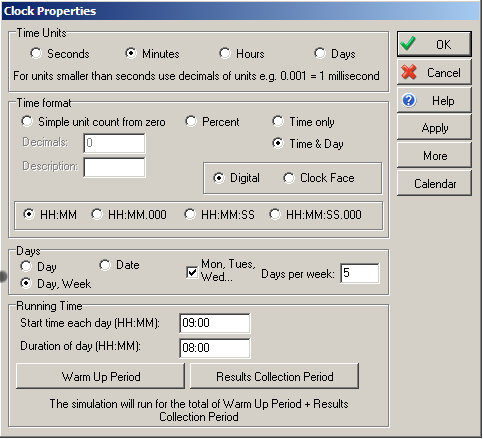
\includegraphics[width=0.75\textwidth]{pic_simul8_clock}
	\caption{Dialog zur Konfiguration der Simulationszeit in Simul8}
	\label{fig:pic_simul8_clock}
\end{figure}

Bei Simul8 besteht zus�tzlich die M�glichkeit, f�r die Dauer eines Tages die Anzahl der Stunden festzulegen. Weiterhin l�sst sich auch die Anzahl der Wochentage festlegen. Eine f�nf Tage Arbeitswoche � acht Stunden kann  beispielsweise wie in Abbildung \ref{fig:pic_simul8_clock} dargestellt f�r eine Simulationsdauer (Result Collecations Period) von 2400 Minuten definiert werden.

\subsubsection{Simprocess}

In Simprocess wird keine Basiseinheit zentral definiert. Daf�r kann jede Zeitangabe in der Simulationssoftware Simprocess exakter und ohne Umrechnung in Bruchzahlen angegeben werden.

Die Simulationsdauer wird durch die Bestimmung der Start- und Endzeit der gesamten Simulation durch Angabe eines konkreten Datums und einer konkreten Uhrzeit festgelegt.

\begin{figure}[H]
	\centering
		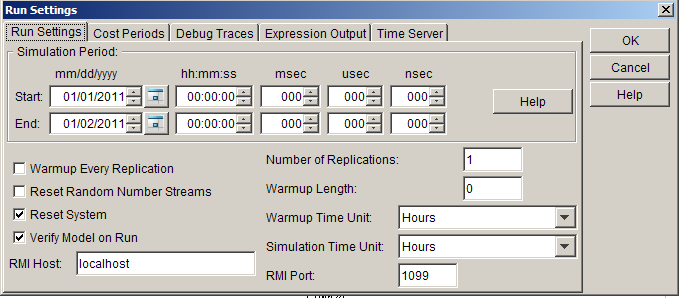
\includegraphics[width=\textwidth]{pic_simprocess_clock}
	\caption{Dialog zur Konfiguration der Simulationszeit in Simprocess}
  \label{fig:pic_simprocess_clock}
\end{figure}

\subsubsection{Micro Saint Sharp}

Simulationszeit wird in Micro Saint Sharp lediglich �ber einen {\em Double}-Wert repr�sentiert.

\subsubsection{Bewertung}

Die verwendeten Ans�tze zur Verwaltung der Simulationszeit unterscheiden sich in allen untersuchten Applikationen recht deutlich voneinander. So mag es sinnvoll sein, sich einmal vor Augen zu f�hren, welche Kriterien eine Verwaltung der Simulationszeit erf�llen soll. Insbesondere die Softwareanwendungen Simprocess und Simul8 sind mit dem Ziel erschaffen worden, Menschen, die begrenzte Kenntnisse in der Programmierung besitzen, anzusprechen. Somit �berrascht es nicht, dass diese Softwaresysteme konkrete Zeitangaben verwenden. Der Vorteil, der sich hieraus ergibt ist eine Art Selbstdokumentation des Simulationsmodells. Weiterhin wird der Modellentwickler dadurch praktisch an die Hand genommen und spart sich verwirrende Umrechnungen in Bruchzahlen. F�r die Pr�sentation einer Simulation ist damit auch weniger Erkl�rungsbedarf vorhanden. Ein nicht zu verachtender Nachteil, der sich aus dieser Herangehensweise ergibt, ist allerdings die Einschr�nkung auf spezielle Anwendungsgebiete. F�r gewisse Anwendungsf�lle kann es sich als n�tzlich erweisen, Basiseinheiten zu verwenden, die unter oder �ber dem Bereich liegen als das, was von der Simulationssoftware erm�glicht wird.

Mirco Saint Sharp verwendet einen Einheitslosen Datentyp, womit gr��tm�gliche Flexibilit�t gewahrt bleibt. Dokumentation dar�ber, welche Zeiteinheit auf diese Einheitslosen Datentyp abgebildet wird, obliegt aber dem Modellentwickler selbst. Schaut man genauer hin, erkennt man, dass die Software Simul8 eine Mischl�sung verwendet, die es Anwendern erlaubt eine Basiseinheit aus vordefinierten Typen zu w�hlen. Die Auswahlm�glichkeiten sind allerdings auch sehr Eingeschr�nkt, sodass der zuvor genannte Nachteil  nicht aufgehoben wird.

Um Zeiteinheiten abzubilden, die zwischen einem Zeitschritt einer gew�hlten Basiseinheit liegen, verwenden Simul8 sowie Micro Saint Sharp Gleitkommazahlen. Gleitkommazahlen sind jedoch nur eine angen�herte Darstellung von den aus der Mathematik bekannten {\em reelen Zahlen}. Ein Vorteil von Gleitkommazahlen ist deren gro�er Wertebereich. Dieser wird allerdings durch eine ungenaue Abbildung auf {\em reelle Zahlen} erkauft. Zwei nahe beieinander liegende reelle Zahlen k�nnen daher in einem ung�nstigen Fall auch auf die selbe Gleitkommazahl abgebildet werden. Auf die Zeitplanung von Ereignissen, die eng beieinander liegen, kann sich das durchaus auswirken. Denn im Zweifelsfall muss die Software entscheiden, welches Ereignis Vorrang hat und in Ermangelung genauer Daten kann dies zu einem Tausch der Reihenfolge f�hren. Fehler k�nnen sich fortsetzen und letztlich das Gesamtergebnis einer Simulation verf�lschen. Betrachtet werden muss also die Wahrscheinlichkeit, mit welcher solch ein Problem auftreten kann und welche Auswirkungen dies auf das Ergebnis hat.
Nun handelt es sich bei dem hier verfolgten Ansatz der Computersimulation  keinesfalls um eine exakte Wissenschaft, als vielmehr um eine Ann�herung an die Realit�t. Somit bleibt es Ermessenssache, inwieweit diese Ungenauigkeiten das Ergebnis einer Computersimulation verf�lschen k�nnen. Generell ist es aber sehr schwierig diese Art von Programmfehlern zu finden. Daher w�rde sich die Verwendung eines stabileren Datentyps anbieten. Ein stabilere Datentyp der einen ebenso gro�en Wertebereich umfasst, wie beispielsweise der Datentyp Double, w�rde selbstredend mit hohen Performance-Einbu�en einhergehen. Da die meisten modernen Prozessoren 64 Bit-Register besitzen, sind f�r die Verwendung von Datentypen, die gr��er als 64 Bit sind, mehr Rechenzyklen f�r sonst gleichwertige Operationen notwendig.

Zusammenfassend soll festgehalten werden, dass die konkrete Wahl eines Ansatzes f�r die Verwaltung von Simulationszeit vom Anwendungsgebiet abh�ngig ist. Da die \Gls{SimNet}-Bibliothek bereits den Datentyp {\em Double} verwendet , ist f�r die angestrebte Eigenentwicklung bereits eine Vorgabe in dieser Angelegenheit gegeben, von der ohne �nderungen in der \Gls{SimNet}-Bibliothek auch nicht abgewichen werden kann. Das .Net Umfeld bietet als einzige Alternative f�r Gleitkommazahlen den 128-Bit Datentyp {\em Decimal}. Dieser besitzt mehr signifikante Stellen als beispielsweise der Datentyp {\em Double}, daf�r ist der verwendete Wertebereich weniger Umfangreich.

\subsection{Aufw�rmphase}

Ziel einer Aufw�rmphase ist es, das System in einen typischen Urzustand zu versetzen. Statistische Daten �ber den Verlauf der Simulation sind ein wichtiges Hilfsmittel, um die Simulation auszuwerten. Solche Daten werden erst nach einer sogenannten {\em WarmUp-Phase} erfasst.  
Eine Aufw�rmphase ist nicht f�r jede Simulation notwendig und wird deshalb von einigen Softwaresystemen optional zur Verf�gung gestellt.\\

\subsubsection{Simul8}

Bei Simul8 geht die Aufw�rmphase nicht in die festgelegte Simulationsdauer mit ein, sondern verl�ngert die tats�chliche Dauer zus�tzlich. Alternativ besteht die M�glichkeit, nach dem Warmup die Simulationszeit auf den Initialwert zur�ckzusetzen.

\subsubsection{Simprocess}

Die Dauer der Aufw�rmphase kann f�r Simprocess direkt festgelegt werden.
Es ist zu beachten, dass die Warmup-Phase direkt mit in die Simulationszeit eingeht
und somit die Statistiken erst nach \begin{math}Startzeit + Warmupzeit\end{math} f�r den Zeitraum \begin{math}Endzeit - Warmupzeit - Startzeit\end{math} erfolgen.

\section{Wahrscheinlichkeitsverteilungen}\label{kap2:verteilungsfunktionen}

Die meisten Ereignisse lassen sich nicht oder nur ungen�gend mit statischen Zeitpunkten und H�ufigkeiten modellieren.
Um beispielsweise die Abl�ufe in einem Callcenter zu simulieren, sind Unregelm��igkeiten beim Eintreffen der Anrufer und der jeweiligen Gespr�chsdauer zu ber�cksichtigen. Statistische Verteilungsfunktionen sind dabei ein vorz�gliches Werkzeug, um solche Problemstellungen anzugehen. Der Tabelle \ref{tab:Distribution} kann entnommen werden, welche Verteilungsfunktionen in welchem Softwarepaket zur Verf�gung stehen. Bei der Bibliothek \Gls{SimNet} handelt es sich um die zugeh�rige Bibliothek f�r die Spracherweiterung der Programmiersprache C\#, welche an der HTW-Dresden entwickelt worden ist. \\

\begin{longtable}{p{55mm}|c|c|c|c}\hline

\footnotesize\textbf{Verteilungsfunktion} & \footnotesize\textbf{Simprocess} & \footnotesize\textbf{Simul8} & \footnotesize\textbf{Micro Saint Sharp} & \footnotesize\textbf{\Gls{SimNet}} \tabularnewline\hline

\endhead

\caption{Statistische Verteilungsfunktionen}
\label{tab:Distribution}%

\endfoot

Bernoulli &


\includegraphics[width=0.4cm, height=0.4cm]{unchecked} &

\includegraphics[width=0.4cm, height=0.4cm]{checked} &

\includegraphics[width=0.4cm, height=0.4cm]{checked} &

\includegraphics[width=0.4cm, height=0.4cm]{unchecked} \tabularnewline\hline

Beta			& 


\includegraphics[width=0.4cm, height=0.4cm]{checked} &

\includegraphics[width=0.4cm, height=0.4cm]{checked} &

\includegraphics[width=0.4cm, height=0.4cm]{checked} &

\includegraphics[width=0.4cm, height=0.4cm]{unchecked} \tabularnewline\hline


Binomial &


\includegraphics[width=0.4cm, height=0.4cm]{checked} &

\includegraphics[width=0.4cm, height=0.4cm]{checked} &

\includegraphics[width=0.4cm, height=0.4cm]{checked} &

\includegraphics[width=0.4cm, height=0.4cm]{unchecked} \tabularnewline\hline

Erlang &


\includegraphics[width=0.4cm, height=0.4cm]{checked} &

\includegraphics[width=0.4cm, height=0.4cm]{checked} &

\includegraphics[width=0.4cm, height=0.4cm]{unchecked} &

\includegraphics[width=0.4cm, height=0.4cm]{checked} \tabularnewline\hline

Exponential &


\includegraphics[width=0.4cm, height=0.4cm]{checked} &

\includegraphics[width=0.4cm, height=0.4cm]{checked} &

\includegraphics[width=0.4cm, height=0.4cm]{checked} &

\includegraphics[width=0.4cm, height=0.4cm]{checked} \tabularnewline\hline

Extreme Value Type A &


\includegraphics[width=0.4cm, height=0.4cm]{unchecked} &

\includegraphics[width=0.4cm, height=0.4cm]{unchecked} &

\includegraphics[width=0.4cm, height=0.4cm]{checked} &

\includegraphics[width=0.4cm, height=0.4cm]{unchecked} \tabularnewline\hline

Extreme Value Type B &


\includegraphics[width=0.4cm, height=0.4cm]{unchecked} &

\includegraphics[width=0.4cm, height=0.4cm]{unchecked} &

\includegraphics[width=0.4cm, height=0.4cm]{checked} &

\includegraphics[width=0.4cm, height=0.4cm]{unchecked} \tabularnewline\hline

Gamma &


\includegraphics[width=0.4cm, height=0.4cm]{checked} &

\includegraphics[width=0.4cm, height=0.4cm]{checked} &

\includegraphics[width=0.4cm, height=0.4cm]{checked} &

\includegraphics[width=0.4cm, height=0.4cm]{unchecked} \tabularnewline\hline

Geometric  &


\includegraphics[width=0.4cm, height=0.4cm]{checked} &

\includegraphics[width=0.4cm, height=0.4cm]{checked} &

\includegraphics[width=0.4cm, height=0.4cm]{checked} &

\includegraphics[width=0.4cm, height=0.4cm]{unchecked} \tabularnewline\hline

Hyper Exponential  &


\includegraphics[width=0.4cm, height=0.4cm]{checked} &

\includegraphics[width=0.4cm, height=0.4cm]{unchecked} &

\includegraphics[width=0.4cm, height=0.4cm]{unchecked} &

\includegraphics[width=0.4cm, height=0.4cm]{unchecked} \tabularnewline\hline

Inverse Gaussian  &


\includegraphics[width=0.4cm, height=0.4cm]{checked} &

\includegraphics[width=0.4cm, height=0.4cm]{unchecked} &

\includegraphics[width=0.4cm, height=0.4cm]{checked} &

\includegraphics[width=0.4cm, height=0.4cm]{unchecked} \tabularnewline\hline

Inverted Weibull  &


\includegraphics[width=0.4cm, height=0.4cm]{checked} &

\includegraphics[width=0.4cm, height=0.4cm]{unchecked} &

\includegraphics[width=0.4cm, height=0.4cm]{unchecked} &
\includegraphics[width=0.4cm, height=0.4cm]{unchecked} \tabularnewline\hline

Johnson SB  &

\includegraphics[width=0.4cm, height=0.4cm]{checked} &
\includegraphics[width=0.4cm, height=0.4cm]{unchecked} &
\includegraphics[width=0.4cm, height=0.4cm]{unchecked} &
\includegraphics[width=0.4cm, height=0.4cm]{unchecked} \tabularnewline\hline

Johnson SU  &

\includegraphics[width=0.4cm, height=0.4cm]{checked} &
\includegraphics[width=0.4cm, height=0.4cm]{unchecked} &
\includegraphics[width=0.4cm, height=0.4cm]{unchecked} &
\includegraphics[width=0.4cm, height=0.4cm]{unchecked} \tabularnewline\hline

Log-Laplace  &

\includegraphics[width=0.4cm, height=0.4cm]{checked} &
\includegraphics[width=0.4cm, height=0.4cm]{unchecked} &
\includegraphics[width=0.4cm, height=0.4cm]{unchecked} &
\includegraphics[width=0.4cm, height=0.4cm]{unchecked} \tabularnewline\hline

Log-Logistic  &

\includegraphics[width=0.4cm, height=0.4cm]{checked} &
\includegraphics[width=0.4cm, height=0.4cm]{unchecked} &
\includegraphics[width=0.4cm, height=0.4cm]{checked} &
\includegraphics[width=0.4cm, height=0.4cm]{unchecked} \tabularnewline\hline

Log-Normal  &

\includegraphics[width=0.4cm, height=0.4cm]{checked} &
\includegraphics[width=0.4cm, height=0.4cm]{checked} &
\includegraphics[width=0.4cm, height=0.4cm]{checked} &
\includegraphics[width=0.4cm, height=0.4cm]{checked} \tabularnewline\hline

Negative Binomial  &

\includegraphics[width=0.4cm, height=0.4cm]{checked} &
\includegraphics[width=0.4cm, height=0.4cm]{checked} &
\includegraphics[width=0.4cm, height=0.4cm]{checked} &
\includegraphics[width=0.4cm, height=0.4cm]{unchecked} \tabularnewline\hline

Normal  &

\includegraphics[width=0.4cm, height=0.4cm]{checked} &
\includegraphics[width=0.4cm, height=0.4cm]{checked} &
\includegraphics[width=0.4cm, height=0.4cm]{checked} &
\includegraphics[width=0.4cm, height=0.4cm]{checked} \tabularnewline\hline

Pareto  &

\includegraphics[width=0.4cm, height=0.4cm]{checked} &
\includegraphics[width=0.4cm, height=0.4cm]{unchecked} &
\includegraphics[width=0.4cm, height=0.4cm]{checked} &
\includegraphics[width=0.4cm, height=0.4cm]{unchecked} \tabularnewline\hline

Pearson Type V  &

\includegraphics[width=0.4cm, height=0.4cm]{checked} &
\includegraphics[width=0.4cm, height=0.4cm]{checked} &
\includegraphics[width=0.4cm, height=0.4cm]{checked} &
\includegraphics[width=0.4cm, height=0.4cm]{unchecked} \tabularnewline\hline

Pearson Type VI  &

\includegraphics[width=0.4cm, height=0.4cm]{checked} &
\includegraphics[width=0.4cm, height=0.4cm]{checked} &
\includegraphics[width=0.4cm, height=0.4cm]{checked} &
\includegraphics[width=0.4cm, height=0.4cm]{unchecked} \tabularnewline\hline

Poisson  &

\includegraphics[width=0.4cm, height=0.4cm]{checked} &
\includegraphics[width=0.4cm, height=0.4cm]{checked} &
\includegraphics[width=0.4cm, height=0.4cm]{unchecked} &
\includegraphics[width=0.4cm, height=0.4cm]{unchecked} \tabularnewline\hline

Random Walk  &

\includegraphics[width=0.4cm, height=0.4cm]{checked} &
\includegraphics[width=0.4cm, height=0.4cm]{unchecked} &
\includegraphics[width=0.4cm, height=0.4cm]{unchecked} &
\includegraphics[width=0.4cm, height=0.4cm]{unchecked} \tabularnewline\hline

Triangular  &

\includegraphics[width=0.4cm, height=0.4cm]{checked} &
\includegraphics[width=0.4cm, height=0.4cm]{checked} &
\includegraphics[width=0.4cm, height=0.4cm]{checked} &
\includegraphics[width=0.4cm, height=0.4cm]{checked} \tabularnewline\hline

Uniform  &

\includegraphics[width=0.4cm, height=0.4cm]{checked} &
\includegraphics[width=0.4cm, height=0.4cm]{checked} &
\includegraphics[width=0.4cm, height=0.4cm]{checked} &
\includegraphics[width=0.4cm, height=0.4cm]{checked} \tabularnewline\hline

Weibull &

\includegraphics[width=0.4cm, height=0.4cm]{checked} &
\includegraphics[width=0.4cm, height=0.4cm]{checked} &
\includegraphics[width=0.4cm, height=0.4cm]{checked} &
\includegraphics[width=0.4cm, height=0.4cm]{checked} \tabularnewline\hline


\end{longtable}

Wie zu erwarten war, sind in allen drei Systemen die wichtigsten Verteilungsfunktionen implementiert. 
Darunter auch einige exotische Varianten, die in der Praxis evtl. nicht so h�ufig Anwendung finden.
Diese Liste zeigt allerdings auch, dass bei der \Gls{SimNet}-Bibliothek in diesem Punkt noch etwas nachger�stet werden kann.

\section{Modell}

Die umfangreichsten und zugleich bedeutendsten Unterschiede zwischen den einzelnen Simulationswerkzeugen sind beim eigentlichen Simulationsmodell zu erkennen. Um nicht den Rahmen zu sprengen, kann dieser Abschnitt nur als Zusammenfassung der wesentlichsten Merkmale dienen. Bevor auf die Details der Realisierung zwischen den einzelnen Simulationspaketen eingegangen werden kann, ist eine Betrachtung der Basiskonzepte notwendig.

\subsection{Basiskonzepte}\label{kap_analyse_modell_basiskonzepte}

Jedes Computermodell besteht aus einer Anzahl von Kanten und Knoten. Zwischen den Knoten entlang der Kanten bewegen sich Token. Die Simulationsbausteine, die im Modell als Knoten dargestellt werden, werden auch als Aktivit�ten bezeichnet und haben einen ma�geblichen Einfluss auf den Verlauf einer Simulation. Die Funktionalit�ten, die durch Aktivit�ten repr�sentiert werden, k�nnen sehr vielseitig sein. So k�nnen Aktivit�ten in das Modell neue Token, d.h. \Glspl{Entitaet}, einf�hren, eingehende Entit�ten vernichten oder an einen anderen verbundenen Zielknoten, d.h. an eine Folgeaktivit�t, weiterleiten. Aktivit�ten werden durch eine F�lle von Merkmalen beschrieben, sodass Modellentwickler �ber die Manipulation der Zust�nde dieser Merkmale das Verhalten einer Aktivit�t innerhalb eines Simulationsmodells beeinflussen k�nnen. Daher werden Aktivit�ten auch nach ihrer Aufgabe voneinander unterschieden. Ein Simulationsmodell besitzt �blicher Weise min. eine Quelle zum Eintritt neuer Entit�ten in das Modell sowie min. eine Senke zum Austritt von Entit�ten aus dem Modell. Un�blich ist hingegen die Modellierung von geschlossenen Systemen ohne Quelle und Senke, denn in solch einem System k�nnen Entit�ten die Simulation weder betreten noch verlassen. Einige Simulationsprogramme, wie beispielsweise Simul8, erlauben allerdings auch die Modellierung von geschlossenen Systemen. In diesem Fall k�nnen Entit�ten bereits f�r den Initialzustand der Simulation als Bestandteil in das Modell integriert sein.
 
\begin{figure}[H]
	\centering
		\includegraphics[width=\textwidth]{pic_modell}
	\caption{Aufbau eines Simulationsmodells}
  \label{fig:pic_modell}
\end{figure}

Der gr��te Unterschied zwischen den untersuchten Simulationspaketen liegt in der Variet�t bei der Gestaltung der Aktivit�ten.
Durch die angestrebte Spezialisierung bzw. Generalisierung bei der Bereitstellung von Modellbausteinen, erkl�rt sich der unterschiedliche Umfang bez�glich der Menge bereitgestellter Aktivit�ten. In der nun folgenden Betrachtung soll daher gezeigt werden, wie sich die unterschiedlichen Ans�tze in der Praxis bew�hren.

\subsection{Simul8}

Wie so oft besitzt auch die Simulationssoftware Simul8 ihre eigene Terminologie. In den allermeisten F�llen stellen die verwendeten Bezeichnungen nur Synonyme f�r bereits vorgestellte Begriffe dar. Um Verwirrung zu vermeiden, ist daher zu erw�hnen, dass Entit�ten in Simul8 als {\em Work Items} bezeichnet werden.

Da sich die Aktivit�ten aus Simul8 recht deutlich voneinander unterscheiden, ist eine Vorbetrachtung gemeinsamer Eigenschaften an dieser Stelle nicht notwendig. 

\begin{figure}[H]
	\centering
		\includegraphics[width=\textwidth]{pic_simul8_modell}
	\caption{Beispiel f�r ein Modell in Simul8}
  \label{fig:pic_simul8_modell}
\end{figure}

\subsubsection{Simulationsbausteine}

\paragraph{Work Entry Point}

\parpic(1cm,1cm)[l][rt]{\includegraphics[width=1cm]{pic_simul8_work_entry_point}}

Der Eintrittspunkt f�r jedes {\em Work Item} stellt der Work Entry Point dar. Dieser kann mit den Generatoren aus anderen \Gls{des}-Systemen verglichen werden. Die wichtigsten Eigenschaften des {\em Work Entry Points} sind in der Tabelle \ref{tab:Work_Entry_Point} aufgef�hrt. \\


\begin{longtable}{p{35mm}|p{11cm}}\hline
\footnotesize\textbf{Eigenschaft} & \footnotesize\textbf{Beschreibung} \tabularnewline\hline

\endhead

\caption{Eigenschaften des Work Entry Points}
\label{tab:Work_Entry_Point}%

\endfoot

Interarrival Time &
Die Ankunftszeiten neuer {\em Work Items} k�nnen �ber Verteilungsfunktionen beschrieben werden. \tabularnewline\hline

Batching &
Die Anzahl der {\em Work Items}, die zum selben Zeitpunkt eintreffen, kann ebenfalls �ber eine Verteilungsfunktion beschrieben werden. \tabularnewline\hline

Routing &
Wenn ein {\em Work Entry Point} mit mehreren Folgeaktivit�ten verbunden ist, muss definiert werden, zu welcher \Gls{Aktivitaet} das {\em Working Item} weitergeleitet wird \tabularnewline\hline

Label Actions &
Vor dem Verlassen eines {\em Work Entry Points} k�nnen Attribute des {\em Work Items} manipuliert werden. Dies kann
insbesondere f�r den sp�teren Programmfluss n�tzlich sein, da diese Attribute von anderen Aktivit�ten ausgewertet werden k�nnen. \tabularnewline\hline

Finance &

F�r die Kostenkalkulation bietet sich eine Festsetzung von Fixkosten ({\em Capital Cost}) f�r den {\em Work Entry Point} und ein Festsetzung von variablen Kosten f�r jede im System eintreffende Einheit an.\tabularnewline\hline

Carbon &
Der Treibhauseffekt wird durch die Festlegung von erzeugten CO2 Emissionen ber�cksichtigt. Analog zu den Finanzen kann ein fester Wert f�r den {\em Work Entry Point} und ein variabler Wert f�r jede im System eintreffende Einheit festgelegt werden.\tabularnewline\hline

Results &

F�r diese Aktivit�t werden unter anderem die folgenden Statistiken gesammelt:
\begin{itemize}
	\item Anzahl eingetroffener {\em Work Items}
	\item Anzahl verloren gegangener {\em Work Items}
	\item Anzahl {\em Work Items}, welche den {\em Work Entry Point} verlassen haben, ohne dabei verloren gegangen zu sein.
\end{itemize}
\tabularnewline\hline

\end{longtable}

\paragraph{Storage Bin}

\parpic(1cm,1cm)[l][rt]{\includegraphics[width=1cm]{pic_simul8_queue}}

Warteschlangen stellen in Simul8 eines der wichtigsten Bestandteile dar. Diese werden am sinnvollsten vor {\em Work Center} plaziert, um {\em Work Items}, die f�r die Bearbeitung in einem Work Center vorgesehen sind, aufzufangen und bereitzuhalten. Tabelle \ref{tab:Storage_Bin} f�hrt die wichtigsten Eigenschaften einer Warteschlange aus Simul8 auf.

\begin{longtable}{p{35mm}|p{11cm}}\hline
\footnotesize\textbf{Eigenschaft} & \footnotesize\textbf{Beschreibung} \tabularnewline\hline



\endhead

\caption{Eigenschaften einer Warteschlange in Simul8}
\label{tab:Storage_Bin}%

\endfoot

Capacity & Die Kapazit�t der Warteschlange ist in der Regel unbegrenzt, kann aber auch auf einen Limit gesetzt werden. \tabularnewline\hline

Shelf Life & Die maximale Verweilszeit eines {\em Work Items} in der Warteschlange kann begrenzt werden.
\tabularnewline\hline

Finance &

F�r die Kostenkalkulation bietet sich eine Festsetzung von Fixkosten ({\em Capital Cost}) f�r die {\em Storage Bin} und eine Festsetzung von variablen Kosten f�r jedes in der Warteschlange befindliche {\em Work Item} pro Zeiteinheit an.\tabularnewline\hline

Carbon &
Der Treibhauseffekt wird durch die Festlegung der von der Warteschlange erzeugten CO2 Emissionen ber�cksichtigt. Analog zu den Finanzen kann ein fester Wert f�r die {\em Storage Bin} und ein variabler Wert f�r jedes in der Warteschlange befindliche {\em Work Item} je Zeiteinheit festgelegt werden.\tabularnewline\hline

Start - Up &
 
Festlegung der Anzahl von {\em Work Items}, welche sich bei Beginn der Simulation in der Warteschlange befinden.\tabularnewline\hline

\Gls{fifo}, PRIORITIZE, LIFO &

Die Reihenfolge, in welcher {\em Work Items} in einer Warteschlange sortiert werden, kann nach folgenden Kriterien erfolgen

\begin{itemize}
	\item First In First Out (Standard)
	\item Last In First Out
	\item Prioritize (Sortierung nach Priorit�t �ber ein {\em Label} (Attribut) des {\em Work Items})
\end{itemize}\tabularnewline\hline
Results &

Auflistung statistischer Werte hinsichtlich der Anzahl von {\em Work Items} in der Warteschlange �ber die Dauer der Simulation.
(Minimum,Maximum,Durchschnitt,Anzahl von eingetroffenen {\em Work Items})

Auflistung statistischer Werte hinsichtlich der Verweildauer von {\em Work Items} in der Warteschlange
(Minimum, Durchschnitt, Maximum, Standardabweichung)\tabularnewline\hline

\end{longtable}

\paragraph{Work Center}

\parpic(1cm,1cm)[l][rt]{\includegraphics[width=1cm]{pic_simul8_work_center}}

Bei dem {\em Work Center} handelt es sich um eine weitere entscheidende Kernkomponente eines jeden Simul8-Modells. Die Bezeichnung {\em Work Center} ist �u�erst passend, denn diese Aktivit�t kann zur Simulation von Arbeit genutzt werden, da Simulationszeit durch das Festhalten von {\em Work Items} voranschreitet, noch bevor ein {\em Work Item} die Aktivit�t wieder verl�sst. Die M�glichkeiten f�r ein {\em Work Center} auf Simulationen einzuwirken sind daher immens. Aufgrund der Komplexit�t dieses Modellbausteins eignet sich ein {\em Work Center} f�r eine Vielzahl von Anwendungsf�llen. Beispielsweise kann ein {\em Work Center} dazu verwendet werden, den Zusammenbau von Einzelkomponenten bei der Fertigung von Produkten zu simulieren. Damit unterscheidet sich Simul8 im Vergleich zu anderen Simulationsprogrammen insofern, dass f�r viele der Anwendungsf�lle, die ein {\em Work Center} abdecken kann, in anderen Softwareprodukten mehrere einzelne Bausteine verwendet werden m�ssen. Insbesondere ist die optimierte Zusammenarbeit mit Warteschlangen und Ressourcen zu erw�hnen. Die wichtigsten Eigenschaften k�nnen aus der Tabelle \ref{tab:Work_Center} entnommen werden.\\



\begin{longtable}{p{35mm}|p{11cm}}\hline
\footnotesize\textbf{Eigenschaft} & \footnotesize\textbf{Beschreibung} \tabularnewline\hline

\endhead

\caption{Eigenschaften eines {\em Work Centers} in Simul8}
\label{tab:Work_Center}%

\endfoot

Distribution & Mittels statistischer Verteilungsfunktionen kann die zu verbrauchende Simulationszeit festgelegt werden,  mit welcher Arbeitszeit simuliert werden soll.
\tabularnewline\hline
Efficency & Es kann festgelegt werden, mit welcher Auslastung das {\em Work Center} arbeitet. Zus�tzlich k�nnen Reparaturzeiten simuliert werden.
\tabularnewline\hline
Priority & Eine Priorit�t kann vergeben werden. Dies ist insbesondere wichtig, wenn mehrere {\em Work Center} um die selben Ressourcen konkurrieren.
\tabularnewline\hline
Label Actions &
Ebenso wie beim {\em Work Entry Point} k�nnen Attribute des {\em Work Items} vor dem verlassen des {\em Work Centers} ver�ndert werden.
\tabularnewline\hline
Replicate &
Festlegung der Anzahl der {\em Work Items}, die im {\em Work Center} gleichzeitig bearbeitet werden k�nnen.
\tabularnewline\hline

Routing In &

Einige Einstellungsoptionen, die regeln, nach welchen Vorgaben ein {\em Work Center} von vorgeschalteten Aktivit�ten {\em Work Items} annimmt. Viele dieser Einstellungen sind nur in Verbindung mit einer Warteschlange sinnvoll. Eine weitere interessante M�glichkeit besteht darin, ein {\em Work Center} durch Arbeit von einem anderen {\em Work Center} unterbrechen zu lassen. Dabei wird das aktuelle {\em Work Item} in eine mit dem {\em Work Center} verbundene Warteschlange geschoben, um sp�ter die Arbeit wieder aufnehmen zu k�nnen.
\tabularnewline\hline

Routing Out &

Wenn ein {\em Work Center} mit mehreren Folgeaktivit�ten verbunden ist, muss definiert werden zu welcher Aktivit�t das {\em Work Item} weitergeleitet wird. \tabularnewline\hline

Contents &

Wenn die Simulation angehalten wird, kann der Inhalt des {\em Work Centers}, dass hei�t die darin befindlichen {\em Work Items} sowie deren Attribute, betrachtet werden.
\tabularnewline\hline

Results &

W�hrend der Simulation werden vom {\em Work Center} Statistiken gesammelt. U.a. sind eine Reihe von Informationen bez�glich der Anzahl der {\em Work Items} im {\em Work Center} verf�gbar. (Aktuell, Maximum, Minimum, Durchschnitt, Anzahl beendeter Jobs).
Viel interessanter sind sicherlich die Werte �ber die Auslastung des {\em Work Centers}. Diese werden in Prozent angegeben und ergeben somit zusammen 100 Prozent. Mit diesen Gr��en kann man neben der tats�chliche Arbeitszeit erkennen, wie lange und weshalb das {\em Work Center} nicht im Betrieb war.
\tabularnewline\hline

Finance &

F�r die Kostenkalkulation bietet sich eine Festsetzung von Fixkosten ({\em Capital Cost}) f�r das {\em Work Center} und eine Festsetzung von St�ckkosten f�r jedes im {\em Work Center} bearbeitete {\em Work Item} an. Au�erdem k�nnen Kosten f�r jede vergangene Zeiteinheit ber�cksichtigt werden.\tabularnewline\hline

\end{longtable}

\paragraph{Work Exit Point}

\parpic(1cm,1cm)[l][rt]{\includegraphics[width=1cm]{pic_simul8_work_exit_point}}


{\em Work Exit Points} dienen in einem Simul8-Modell als Senke. Wenn beispielsweise ein {\em Work Item} einen {\em Work Exit Point} erreicht hat, so verl�sst es �ber diesen die Simulation.
Im Vergleich zu anderen Modellbausteinen in Simul8 ist der {\em Work Exit Point} weniger komplex. In der Tabelle \ref{tab:Work_Exit_Point} werden die wichtigsten Eigenschaften des {\em Work Exit Points} aufgez�hlt \\



\begin{longtable}{p{35mm}|p{11cm}}\hline
\footnotesize\textbf{Eigenschaft} & \footnotesize\textbf{Beschreibung} \tabularnewline\hline

\endhead

\caption{Eigenschaften eines {\em Work Exit Points} in Simul8}
\label{tab:Work_Exit_Point}%

\endfoot

Halt Simulation at Limit & Nach Erreichen einer definierten maximalen Anzahl von {\em Work Items} die am {\em Work Exit Point} eintreffen, wird die Simulation beendet\tabularnewline\hline

Finance &
Festsetzung von Fixkosten ({\em Capital Cost}) f�r den {\em Work Exit Point}. Weiterhin k�nnen Einnahmen in Form eines St�ckpreises({\em Revenue Costs}) pro {\em Work Item}, welche �ber diese Senke die Simulation verlassen, definiert werden\tabularnewline\hline

Carbon &

Der Treibhauseffekt wird durch die Festlegung der erzeugten CO2 Emissionen ber�cksichtigt.  Analog zu den Finanzen kann ein Wert f�r den {\em Work Exit Point} festgelegt werden. Zudem ist es m�glich, eine Verringerung der CO2 Emissionen f�r jede die Simulation verlassende Einheit zu definieren.\tabularnewline\hline

Results &

\begin{itemize}
	\item Statistiken �ber die Verweildauer der {\em Work Items} in der Simulation (Minimum, Durchschnitt, Maximum, Standardabweichung)
	\item Anzahl {\em Work Items}, die �ber diesen {\em Work Exit Point} die Simulation verlassen haben
\end{itemize}
\tabularnewline\hline
 



\end{longtable}

\paragraph{Resource}

\parpic(1cm,1cm)[l][rt]{\includegraphics[width=1cm]{pic_simul8_resources}}

Ressourcen k�nnen in Simul8 als grafischer Baustein in das Modell integriert werden. Aber im Gegensatz zu den bisher vorgestellten Simulationsbausteinen sind Ressourcen keine Aktivit�ten und daher nicht �ber Kanten mit anderen Simulationsbausteinen verbunden. {\em Work Center} k�nnen um Ressourcen konkurrieren. Damit eignen sich Ressourcen vorz�glich, um Abh�ngigkeiten zu simulieren. Die Tabelle \ref{tab:Simul8_Resources} enth�lt eine Auflistung der wichtigsten Eigenschaften von Ressourcen in Simul8. \\

\begin{longtable}{p{35mm}|p{11cm}}\hline
\footnotesize\textbf{Eigenschaft} & \footnotesize\textbf{Beschreibung} \tabularnewline\hline

\endhead

\caption{Eigenschaften einer {\em Ressource} in Simul8}
\label{tab:Simul8_Resources}%

\endfoot


Travel & Definition von Reisezeiten f�r Ressourcen. \tabularnewline\hline
Availability & Festlegung eines Prozentsatzes f�r die Verf�gbarkeit der Ressource. \tabularnewline\hline
Shifts & Ein sehr hilfreiches Feature ist die Bestimmung von Arbeitsschichten, womit die Verf�gbarkeit von Ressourcen ebenfalls eingeschr�nkt werden kann.\tabularnewline\hline
Finance & Definition von Fixkosten f�r jede Einheit und variable Kosten je Zeiteinheit. \tabularnewline\hline
Carbon & Der Treibhauseffekt wird durch die Festlegung der erzeugten CO2 Emissionen ber�cksichtigt. Es kann ein fester Wert f�r jede Einheit einer Ressource festgelegt werden. Au�erdem kann die Erzeugung von CO2 Emissionen je Zeiteinheit, f�r die eine Ressourceneinheit belegt ist, definiert werden.\tabularnewline\hline
Results & Es werden Statistiken �ber die Auslastung und Reisezeiten f�r alle Einheiten der Resource erfasst.\tabularnewline\hline


\end{longtable}


\subsubsection{Bewertung}

Die Anzahl der Aktivit�ten im Simulationspaket Simul8 ist recht �berschaubar. Insgesamt gibt es lediglich sechs verschiedene Bausteine, wovon die f�nf wichtigsten in dem vorangegangen Abschnitt betrachtet worden sind. Dies hat zur Folge, dass es kaum Elemente gibt, auf die man f�r ein Simulationsmodell verzichten wird. Ein Vorteil ist sicherlich die schnellere und unkompliziertere Erlernbarkeit der Anwendung. Allerdings muss auch ber�cksichtigt werden, dass evtl. umfangreiche Simulationen intensiver kommentiert werden m�ssen. Denn die Wirkungsweise einzelner Komponenten ist nicht in jedem Fall selbsterkl�rend, da vieles was in anderen Simulationspaketen wie z.B.: Simprocess �ber zus�tzliche Aktivit�ten (u.a. Routing, Assembling) realisiert wird, in einzelne Simulationsbausteine von Simul8 direkt integriert ist. Abgesehen von Quellen und Senken ist ein Simulationsmodell in Simul8 somit haupts�chlich aus Warteschlangen und {\em Work Center} aufgebaut. Ein weiterer Nachteil, der aus dieser Herangehensweise resultiert, ist, dass nicht jede Aktivit�t mit jeder anderen Aktivit�t gleich gut zusammenarbeitet. So sind viele Optionen des {\em Work Centers} f�r die Zusammenarbeit mit Warteschlangen ausgelegt. Einige dieser Optionen machen im Zusammenhang mit anderen Komponenten allerdings keinen Sinn und k�nnen sogar f�r Deadlocks sorgen. Es ist anzumerken, dass aus dieser Betrachtung einige Erkenntnisse f�r die angestrebte Eigenentwicklung gewonnen werden konnten. Viele der hier vorgestellten Funktionalit�ten, die in Simul8 existieren, werden auch ihren Weg in die aus dieser Arbeit hervorgehende Softwarel�sung finden. Allerdings erscheint es mit Bezug auf die eigene Implementation  als ein konsistenterer Ansatz, Funktionalit�ten auf mehrere Simulationsbausteine aufzuteilen. Dies erleichtert insbesondere auch die Programmierung der Kommunikation der verschiedenen Komponenten untereinander, womit die Endl�sung weniger fehleranf�llig sein sollte.

\subsection{Simprocess}

In Simprocess werden Token, die sich durch das Simulationsmodell bewegen als Entit�ten (engl. Entity) bezeichnet.

Viele Aktivit�ten besitzen �hnliche Eigenschaften, sodass die allgemeinen Besonderheiten vor der Betrachtung der einzelnen Aktivit�ten in diesem Abschnitt vorweggenommen werden sollen.

F�r die Kommunikation untereinander besitzen Aktivit�ten sogenannte Pads. Dabei kann eine Aktivit�t mehrere Input-Pads sowie Output-Pads
mit unterschiedlichen Aufgaben besitzen. Input-Pads erlauben eine unbegrenzte Anzahl an eingehenden Verbindungen, w�hrend die meisten Output-Pads hingegen nur auf eine ausgehende Verbindung beschr�nkt sind. Es gibt allerdings auch Ausnahmen, wie beispielsweise bei der Split-Aktivit�t, die in Kapitel \ref{kap:simprocess_split} auf Seite \pageref{kap:simprocess_split} n�her beschrieben wird.

Eine elementare Eigenschaft der meisten Aktivit�ten ist es, Simulationszeit verbrauchen zu k�nnen, indem die Dauer eines Prozesses, der durch die Aktivit�t repr�sentiert wird, mittels einer Wahrscheinlichkeitsverteilung beschrieben wird. Eine Besonderheit in Simprocess ist, dass es keinen extra Baustein f�r Warteschlangen gibt. Stattdessen ist in allen Aktivit�ten, die Simulationszeit verbrauchen k�nnen, eine Warteschlange integriert.
Generatoren stellen in diesem Zusammenhang eine Ausnahme dar, da diese als Quelle keine Input-Pads besitzen. 

Auch in Simprocess spielen Ressourcen eine wichtige Rolle. Aktivit�ten k�nnen von Ressourcen abh�ngig sein und ihre Arbeit blockieren, bis ihnen die n�tigen Ressourcen zur Verf�gung stehen. Zudem k�nnen f�r Ressourcen ebenfalls Kosten definiert werden, womit diese auch als ein Werkzeug f�r die Kalkulation von Lohn und Betriebskosten eingesetzt werden k�nnen. Mittels eines sogenannten {\em Schedules} l�sst sich �berdies die Verf�gbarkeit von Ressourcen einschr�nken, um beispielsweise Arbeitszeiten zu simulieren.

Simprocess erlaubt es f�r Entit�ten, Aktivit�ten und Ressourcen eine Vielzahl von Statistiken zu sammeln. Ausgew�hlte Statistiken k�nnen nach einem Simulationslauf in Form eines Protokolls in einem Texteditor betrachtet werden.

Die folgende Tabelle \ref{tab:simprocess_activities} fasst die Einzelheiten f�r die in dieser Arbeit betrachteten Aktivit�ten aus der Simulationssoftware Simprocess zusammen.\\\begin{longtable}{m{0.35cm}|m{2.5cm}|m{2.5cm}|m{2.6cm}|m{1.8cm}|m{1.35cm}|m{1.30cm}}\hline
 & \footnotesize\textbf{Aktivit�t} & \footnotesize\textbf{Warteschlange} & \footnotesize\textbf{Simulationszeit} & \footnotesize\textbf{Ressourcen} & \footnotesize\textbf{Input-Pads} & \footnotesize\textbf{Output-Pads} \tabularnewline\hline

 
\endhead

\caption{Aktivit�ten in Simprocess}
\label{tab:simprocess_activities}%

\endfoot


 
\centering\includegraphics[width=0.4cm]{pic_simprocess_generator.png} &
Generate &
\centering\includegraphics[width=0.45cm, height=0.45cm]{unchecked} &
\centering\includegraphics[width=0.45cm, height=0.45cm]{checked} &
\centering\includegraphics[width=0.45cm, height=0.45cm]{unchecked} &
\centering 0 & 
\centering 1 \tabularnewline\hline

\centering\includegraphics[height=0.4cm]{pic_simprocess_dispose.png} &
Dispose & 
\centering\includegraphics[width=0.45cm, height=0.45cm]{checked} &
\centering\includegraphics[width=0.45cm, height=0.45cm]{unchecked} &
\centering\includegraphics[width=0.45cm, height=0.45cm]{unchecked} &
\centering 1 &
\centering 0 \tabularnewline\hline 


\centering\includegraphics[height=0.4cm]{pic_simprocess_delay.png} &
Delay & 
\centering\includegraphics[width=0.45cm, height=0.45cm]{checked} &
\centering\includegraphics[width=0.45cm, height=0.45cm]{checked} &
\centering\includegraphics[width=0.45cm, height=0.45cm]{checked} &
\centering 1 &
\centering 1 \tabularnewline\hline 

\centering\includegraphics[height=0.4cm]{pic_simprocess_assemble.png} &
Assemble & 
\centering\includegraphics[width=0.45cm, height=0.45cm]{checked} &
\centering\includegraphics[width=0.45cm, height=0.45cm]{checked} &
\centering\includegraphics[width=0.45cm, height=0.45cm]{checked} &
\centering 2 &
\centering 2 \tabularnewline\hline 

\centering\includegraphics[height=0.4cm]{pic_simprocess_branch.png} &
Branch & 
\centering\includegraphics[width=0.45cm, height=0.45cm]{checked} &
\centering\includegraphics[width=0.45cm, height=0.45cm]{checked} &
\centering\includegraphics[width=0.45cm, height=0.45cm]{checked} &
\centering 1 &
\centering 1 \tabularnewline\hline

\centering\includegraphics[height=0.4cm]{pic_simprocess_branch.png} &
Merge & 
\centering\includegraphics[width=0.45cm, height=0.45cm]{unchecked} &
\centering\includegraphics[width=0.45cm, height=0.45cm]{unchecked} &
\centering\includegraphics[width=0.45cm, height=0.45cm]{unchecked} &
\centering 1 &
\centering 1 \tabularnewline\hline


\centering\includegraphics[height=0.4cm]{pic_simprocess_batch.png} &
Batch & 
\centering\includegraphics[width=0.45cm, height=0.45cm]{checked} &
\centering\includegraphics[width=0.45cm, height=0.45cm]{checked} &
\centering\includegraphics[width=0.45cm, height=0.45cm]{checked} &
\centering 1 &
\centering 1 \tabularnewline\hline 

\centering\includegraphics[height=0.4cm]{pic_simprocess_unbatch.png} &
Unbatch & 
\centering\includegraphics[width=0.45cm, height=0.45cm]{checked} &
\centering\includegraphics[width=0.45cm, height=0.45cm]{checked} &
\centering\includegraphics[width=0.45cm, height=0.45cm]{checked} &
\centering 1 &
\centering 1 \tabularnewline\hline

\centering\includegraphics[height=0.4cm]{pic_simprocess_split.png} &
Split & 
\centering\includegraphics[width=0.45cm, height=0.45cm]{checked} &
\centering\includegraphics[width=0.45cm, height=0.45cm]{checked} &
\centering\includegraphics[width=0.45cm, height=0.45cm]{checked} &
\centering 1 &
\centering 2 \tabularnewline\hline 

\centering\includegraphics[height=0.4cm]{pic_simprocess_join.png} &
Join & 
\centering\includegraphics[width=0.45cm, height=0.45cm]{checked} &
\centering\includegraphics[width=0.45cm, height=0.45cm]{checked} &
\centering\includegraphics[width=0.45cm, height=0.45cm]{checked} &
\centering 1 &
\centering 2 \tabularnewline\hline

\centering\includegraphics[height=0.4cm]{pic_simprocess_transform.png} &
Transform & 
\centering\includegraphics[width=0.45cm, height=0.45cm]{checked} &
\centering\includegraphics[width=0.45cm, height=0.45cm]{checked} &
\centering\includegraphics[width=0.45cm, height=0.45cm]{checked} &
\centering 1 &
\centering 1 \tabularnewline\hline

\centering\includegraphics[height=0.4cm]{pic_simprocess_transfer.png} &
Transfer & 
\centering\includegraphics[width=0.45cm, height=0.45cm]{unchecked} &
\centering\includegraphics[width=0.45cm, height=0.45cm]{unchecked} &
\centering\includegraphics[width=0.45cm, height=0.45cm]{unchecked} &
\centering 0/1 &
\centering 0/1 \tabularnewline\hline


\centering\includegraphics[height=0.4cm]{pic_simprocess_gate.png} &
Gate & 
\centering\includegraphics[width=0.45cm, height=0.45cm]{checked} &
\centering\includegraphics[width=0.45cm, height=0.45cm]{checked} &
\centering\includegraphics[width=0.45cm, height=0.45cm]{checked} &
\centering 2 &
\centering 1 \tabularnewline\hline

\centering\includegraphics[height=0.4cm]{pic_simprocess_assign.png} &
Assign & 
\centering\includegraphics[width=0.45cm, height=0.45cm]{checked} &
\centering\includegraphics[width=0.45cm, height=0.45cm]{checked} &
\centering\includegraphics[width=0.45cm, height=0.45cm]{checked} &
\centering 1 &
\centering 1 \tabularnewline\hline 

\centering\includegraphics[height=0.4cm]{pic_simprocess_synchronize.png} &
Synchronize & 
\centering\includegraphics[width=0.45cm, height=0.45cm]{checked} &
\centering\includegraphics[width=0.45cm, height=0.45cm]{checked} &
\centering\includegraphics[width=0.45cm, height=0.45cm]{checked} &
\centering variabel &
\centering variabel \tabularnewline\hline

\centering\includegraphics[height=0.4cm]{pic_simprocess_getresource.png} &
Get Resource & 
\centering\includegraphics[width=0.45cm, height=0.45cm]{checked} &
\centering\includegraphics[width=0.45cm, height=0.45cm]{unchecked} &
\centering\includegraphics[width=0.45cm, height=0.45cm]{checked} &
\centering 1 &
\centering 1 \tabularnewline\hline


\centering\includegraphics[height=0.4cm]{pic_simprocess_freeresource.png} &
Free Resource & 
\centering\includegraphics[width=0.45cm, height=0.45cm]{unchecked} &
\centering\includegraphics[width=0.45cm, height=0.45cm]{unchecked} &
\centering\includegraphics[width=0.45cm, height=0.45cm]{checked} &
\centering 1 &
\centering 1 \tabularnewline\hline 

\end{longtable}

\subsubsection{Simulationsbausteine}

\paragraph{Generate}

\parpic(1cm,1cm)[l][rt]{\includegraphics[width=1cm]{pic_simprocess_generator.png}}

Generatoren dienen in Simprocess als Quelle f�r das Simulationsmodell. Diese erzeugen gem�� eines Plans (engl. {\em Schedule}) neue Entit�ten.
Hiervon existieren eine Reihe von unterschiedlichen Arten, wovon die wichtigsten in der Tabelle \ref{tab:simprocess_schedule} zusammengefasst werden.
Eine Besonderheit ist, dass einem Generator mehrere solcher {\em Schedules} zugewiesen werden k�nnen. Womit ein Generator in die Lage versetzt wird, verschiedene Typen von Entit�ten zu erzeugen. \\


\begin{longtable}{p{35mm}|p{11cm}}\hline
\footnotesize\textbf{Scheduletyp} & \footnotesize\textbf{Beschreibung} \tabularnewline\hline

\endhead

\caption{Schedulearten in Simprocess}
\label{tab:simprocess_schedule}%

\endfoot

Periodic & 
Der {\em Periodic Schedule} ist wohl der am h�ufigsten verwendete Scheduletyp in Simprocess.
�ber statistische Verteilungsfunktionen kann �ber solch einen Plan der Rhythmus zur Erzeugung von Entit�ten bestimmt werden. Ebenfalls kann �ber eine Verteilungsfunktion die Anzahl der Entit�ten bestimmt werden, die zum selben Zeitpunkt im Simulationsmodell eintreffen. \tabularnewline\hline
Calendar &
Der {\em Calendar Schedule} kann wie der {\em Periodic Schedule} �ber statistische Verteilungsfunktionen die Anzahl der Entit�ten bestimmen, die zum selben Zeitpunkt erzeugt werden sollen. Die Besonderheit liegt aber darin, dass feste Zeitpunkte bestimmt werden k�nnen, wann neue Entit�ten im Simulationsmodell eintreffen. Beispielsweise kann ein exaktes Datum oder aber eine exakte Definition von monatlich, w�chentlich, t�glich oder st�ndlich verwendet werden.  
\tabularnewline\hline
Weekly &
Der {\em Weekly Schedule} ist im Prinzip eine Erweiterung des {\em Periodic Schedules}. Einzig wird die M�glichkeit erg�nzt, Zeitr�ume festzulegen, innerhalb welcher dieser Schedule aktiv ist. N�tzlich ist dies, um beispielsweise Arbeitszeiten zu simulieren.\tabularnewline\hline

\end{longtable}

\paragraph{Dispose}

\parpic(1cm,1cm)[l][rt]{\includegraphics[width=1cm]{pic_simprocess_dispose.png}}

Das Gegenst�ck zu {\em Generate} ist der {\em Dispose} Baustein. �ber diesen verlassen Entit�ten das Simulationsmodell. {\em Dispose} kann auch dazu verwendet werden, die Simulation vorzeitig abzubrechen, indem eine Maximalanzahl von Entit�ten bestimmt wird. Dabei muss es sich nicht um einen festen Wert handeln, denn auch die Verteilungsfunktionen, die in der Tabelle \ref{tab:Distribution} auf Seite \pageref{tab:Distribution} in der Spalte Simprocess aufgelistet worden sind, k�nnen verwendet werden.

\newpage
\paragraph{Delay}

\parpic(1cm,1cm)[l][rt]{\includegraphics[width=1cm]{pic_simprocess_delay.png}}

Eine der elementarsten Komponente ist sicherlich die {\em Delay}-Aktivit�t. Diese wird eingesetzt, um ankommende Entit�ten f�r einen festgelegten Zeitraum zu blockieren.

\paragraph{Assemble}

\parpic(1cm,1cm)[l][rt]{\includegraphics[width=1cm]{pic_simprocess_assemble.png}}

{\em Assemble} kann verwendet werden, um beispielsweise den Zusammenbau von Komponenten zu simulieren. Notwendige Materialien werden in Form von Entit�ten gesammelt. Die Gesamtheit der ben�tigten Materialien kann sich aus unterschiedlichen Entit�tstypen zusammensetzen. Dabei l�sst sich auch die Anzahl der notwendigen Entit�ten �ber statistische Verteilungsfunktionen definieren. Sobald eine {\em Assemble}-Aktivit�t die notwendigen Materialien hat, beginnt diese mit der Arbeit. Zuletzt muss noch der Entit�tstyp f�r die zu erzeugende Entit�t festgelegt werden. Da es im Gegensatz zu vielen anderen Aktivit�ten mehrere Input- und Output-Pads gibt, werden diese in der Tabelle \ref{tab:simprocess_assemble_pads} aufgef�hrt.\\

\begin{longtable}{p{3.8cm}|p{1.4cm}|p{9.3cm}}\hline
\footnotesize\textbf{Pad} & \footnotesize\textbf{Typ} & \footnotesize\textbf{Beschreibung} \tabularnewline\hline


\endhead

\caption{Schedulearten in Simprocess}
\label{tab:simprocess_assemble_pads}%

\endfoot


Trigger (Optional) & Input & 
Die {\em Assemble}-Aktivit�t kann zus�tzlich auf einen Trigger warten, dieser wird ausgel�st, sobald die Aktivit�t von einer Entit�t �ber
den Trigger-Pad erreicht worden ist. Die eintreffende Entit�t wird sofort vernichtet und landet damit nicht in der Warteschlange der {\em Assemble}-Aktivit�t.
\tabularnewline\hline
Component & Input &
Entit�ten, die als Material f�r die Fertigung verwendet werden sollen, erreichen die {\em Assemble}-Aktivit�t �ber dieses Pad.
\tabularnewline\hline
Out & Output &
Erzeugte Entit�ten verlassen die {\em Assemble}-Aktivit�t �ber dieses Pad.
\tabularnewline\hline
NoMatch (Optional) & Output &
Entit�ten, die f�r den Fertigungsprozess nicht verwendet werden k�nnen, k�nnen �ber dieses Pad die {\em Assemble}-Aktivit�t wieder verlassen
\tabularnewline\hline

\end{longtable}


\paragraph{Branch}

\parpic(1cm,1cm)[l][rt]{\includegraphics[width=1cm]{pic_simprocess_branch.png}}

Die {\em Branch}-Aktivit�t kann als Abzweigung eintreffende Entit�ten auf verschiedenen Wegen zu verbundenen Aktivit�ten weiterleiten. Die Tabelle \ref{tab:simprocess_branch} listet die m�glichen Arten der Abzweigung auf. \\

\begin{longtable}{p{35mm}|p{11cm}}\hline
\footnotesize\textbf{Abzweigungsart} & \footnotesize\textbf{Beschreibung} \tabularnewline\hline

\endhead

\caption{Abzweigungsvarianten f�r die {\em Branch}-Aktivit�t in Simprocess}
\label{tab:simprocess_branch}%

\endfoot

Probability & Die Wahrscheinlichkeit bestimmt, welcher Weg  gew�hlt wird. Die Wahrscheinlichkeit f�r alle angeschlossenen Verbindungen muss insgesamt 1.0 betragen.  \tabularnewline\hline

Attribute & F�r die Wahl des Weges k�nnen auch Attribute von Entit�ten der Aktivit�t oder dem Modell herangezogen werden. �ber Vergleichsoperationen wird entschieden, welchen Weg eine Entit�t w�hlt.
\tabularnewline\hline

Entity Type & Der Typ der Entit�t kann ebenfalls als ausschlaggebendes Kriterium bei der Wahl des Weges herangezogen werden.
\tabularnewline\hline

Priority & Bei der Priorit�t handelt es sich lediglich um eine Komfortfunktion, denn diese ist im Grunde auch nur ein Attribut der Entit�t.\tabularnewline\hline

\end{longtable}

\paragraph{Merge}

\parpic(1cm,1cm)[l][rt]{\includegraphics[width=1cm]{pic_simprocess_merge.png}}

Die {\em Merge}-Aktivit�t kann als Gegenst�ck zur {\em Branch}-Aktivit�t betrachtet werden. Alle eintreffenden Entit�ten werden auf dem selben Weg weiter versandt. Diese Aktivit�t ist nicht unbedingt notwendig, da alle InputPads genau nach eben diesem Prinzip arbeiten. Allerdings hilft sie, die  Struktur des Simulationsmodells �bersichtlicher zu gestalten. Au�erdem erhalten alle eintreffenden Entit�ten, wie bei jeder anderen Aktivit�t, einen neuen Zeitstempel \footnote{Vgl. \cite{USM20008} S. 141}. Im Gegensatz zu den meisten anderen Aktivit�ten kann die {\em Merge} Aktivit�t daher auch keine Simulationszeit verbrauchen oder Ressourcen verwenden.

\newpage
\paragraph{Batch}

\parpic(1cm,1cm)[l][rt]{\includegraphics[width=1cm]{pic_simprocess_batch.png}}

Die {\em Batch}-Aktivit�t fasst eine zuvor bestimmte Anzahl von Entit�ten zu einer neuen Entit�t zusammen.
Je nach Einstellung m�ssen zus�tzliche Kriterien erf�llt sein, bevor mit dem {\em Batch}-Prozess begonnen wird. 
Ist die maximale Aufenthaltsdauer f�r Entit�ten in der Warteschlange erreicht sowie das Kriterium f�r die minimale Anzahl von Entit�ten in der Warteschlange erf�llt, wird der {\em Batch}-Prozess gestartet. Weiterhin k�nnen eingehende Entit�ten nach der Priorit�t oder dem Typ der Entit�t getrennt werden.

\paragraph{Unbatch}

\parpic(1cm,1cm)[l][rt]{\includegraphics[width=1cm]{pic_simprocess_unbatch.png}}

Die {\em Unbatch}-Aktivit�t kehrt den Prozess der {\em Batch}-Aktivit�t um, indem sie Entit�ten, die sich in eintreffenden Container-Entit�ten befinden, auspackt. Dabei besteht die Option, auch verschachtelte Pakete zu ber�cksichtigen. Container-Entit�ten k�nnen je nach Einstellung ebenfalls erhalten bleiben.

\paragraph{Split}
\label{kap:simprocess_split}

\parpic(1cm,1cm)[l][rt]{\includegraphics[width=1cm]{pic_simprocess_split.png}}

Mit der {\em Split}-Aktivit�t lassen sich von einer eintreffenden Entit�t beliebig viele Kopien erstellen. F�r das sp�tere Zusammenf�hren der Kopien mit dem Original wird ein Familienname vergeben. Eine Beschreibung der beiden Output-Pads kann der Tabelle \ref{tab:simprocess_split_pads} entnommen werden.\\

\begin{longtable}{p{35mm}|p{11cm}}\hline
\footnotesize\textbf{Output-Pad} & \footnotesize\textbf{Beschreibung} \tabularnewline\hline


\endhead

\caption{Output-Pads der {\em Split}-Aktivit�t}
\label{tab:simprocess_split_pads}%

\endfoot

Original &
�ber dieses Pad verlassen Original-Entit�ten die {\em Split}-Aktivit�t.
\tabularnewline\hline

Clones &
Kopien des Originals verlassen �ber dieses Pad die {\em Split}-Aktivit�t.
Mit diesem Pad k�nnen �ber einen {\em Connector} beliebig viele Aktivit�ten verbunden werden. 
Die Anzahl der Verbindungen entspricht somit der Anzahl der Klone.\tabularnewline\hline

\end{longtable}


\paragraph{Join}

\parpic(1cm,1cm)[l][rt]{\includegraphics[width=1cm]{pic_simprocess_join.png}}

Die {\em Join}-Aktivit�t dient zur Zusammenf�hrung der Originale mit ihren Kopien, wie sie von der {\em Split}-Aktivit�t erzeugt worden sind. Dabei befinden sich Kopien und Originale so lange in der Warteschlange der {\em Join}-Aktivit�t, bis alle zugeh�rigen Komponenten eingesammelt worden sind. Die Join-Aktivit�t besitzt zwei Output-Pads, deren Beschreibung der Tabelle \ref{tab:simprocess_join_pads} entnommen werden kann.\\

\begin{longtable}{p{35mm}|p{11cm}}\hline
\footnotesize\textbf{Output-Pad} & \footnotesize\textbf{Beschreibung} \tabularnewline\hline


\endhead

\caption{Output-Pads der {\em Join}-Aktivit�t}
\label{tab:simprocess_join_pads}%

\endfoot

Join &
�ber dieses Pad verlassen Original-Entit�ten die {\em Join}-Aktivit�t.
\tabularnewline\hline

NoMatch &
Dieses Output-Pad dient zur Aussortierung von Entit�ten, die f�r eine Join-Operation nicht in Frage kommen.\tabularnewline\hline

\end{longtable}

\paragraph{Transform}

\parpic(1cm,1cm)[l][rt]{\includegraphics[width=1cm]{pic_simprocess_transform.png}}

Die {\em Transform}-Aktivit�t wandelt den Typ von eintreffenden Entit�ten in einen anderen Typ um. Dabei k�nnen globale Attribute sowie der Erstellungszeitpunkt, die Zeitstempel und die Priorit�t der urspr�nglichen Entit�t �bernommen werden.


\paragraph{Transfer}

\parpic(1cm,1cm)[l][rt]{\includegraphics[width=1cm]{pic_simprocess_transfer.png}}

Die {\em Transfer}-Aktivit�t unterscheidet sich von allen bisher vorgestellten Aktivit�ten entscheidend. {\em Transfer}-Aktivit�ten stellen
eine M�glichkeit dar, auch ohne Verbindungen Entit�ten an andere {\em Transfer}-Aktivit�ten weiterzuleiten. Bei {\em Transfer}-Aktivit�ten muss zwischen zwei verschiedenen Zust�nden unterschieden werden. In der Tabelle \ref{tab:simprocess_transfer_modus} werden die Unterschiede erl�utert.\\

\begin{longtable}{p{3.5cm}|p{11cm}}\hline
\footnotesize\textbf{Modus} & \footnotesize\textbf{Beschreibung} \tabularnewline\hline

\endhead

\caption{Zust�nde der {\em Transfer}-Aktivit�t}
\label{tab:simprocess_transfer_modus}%

\endfoot

Send & Befindet sich eine {\em Transfer}-Aktivit�t im {\em Send}-Zustand, besitzt diese ein Input-Pad und es werden alle eingehenden Entit�ten an die {\em Transfer}-Aktivit�t weitergeleitet, die als Empf�nger definiert worden ist. \tabularnewline\hline

Receive & Eine {\em Transfer}-Aktivit�t, die sich im {\em Receive}-Zustand befindet, kann von beliebig vielen {\em Transfer}-Aktivit�ten Entit�ten empfangen. In der Folge werden alle eingetroffenen Entit�ten an die �ber das Output-Pad angebundene Aktivit�t weitergeleitet.\tabularnewline\hline

\end{longtable}

\paragraph{Gate}

\parpic(1cm,1cm)[l][rt]{\includegraphics[width=1cm]{pic_simprocess_gate.png}}

Die {\em Gate}-Aktivit�t sammelt eingehende Entit�ten und h�lt diese solange in ihrer Warteschlange auf, bis entweder die Anzahl der Entit�ten in der Warteschlange gr��er als eine definierte Schranke ist oder eine Entit�t �ber das {\em Trigger}-Pad die {\em Gate}-Aktivit�t erreicht hat.

\paragraph{Assign}

\parpic(1cm,1cm)[l][rt]{\includegraphics[width=1cm]{pic_simprocess_assign.png}}

Die {\em Assign}-Aktivit�t stellt eine einfache M�glichkeit dar, um Werte von benutzerdefinierten Attributen sowie Priorit�ten f�r Entit�ten zu definieren.


\paragraph{Synchronize}

\parpic(1cm,1cm)[l][rt]{\includegraphics[width=1cm]{pic_simprocess_synchronize.png}}

Die {\em Synchronize}-Aktivit�t besitzt eine variable Anzahl von Input- und Output-Pads. Sobald an jedem Eingang der Aktivit�t jeweils mindestens eine Entit�t eingetroffen ist, werden an allen korrespondierenden Ausg�ngen Entit�ten wieder freigelassen.

\newpage
\paragraph{Get Resource}


\parpic(1cm,1cm)[l][rt]{\includegraphics[width=1cm]{pic_simprocess_getresource.png}}

H�ufig ist es eine Notwendigkeit, eine Ressource f�r eine Abfolge von Aktivit�ten zu belegen. Mit der Aktivit�t {\em Get Resource} ist dies m�glich. Wenn eine Entit�t bei dieser Aktivit�t angelangt ist und sofern eine Ressource bereitsteht, darf die Entit�t die {\em Get Resource} Aktivit�t wieder verlassen. In jedem anderen Fall werden eingehende Entit�ten in der Warteschlange der Aktivit�t aufbewahrt.

\paragraph{Free Resource}

\parpic(1cm,1cm)[l][rt]{\includegraphics[width=1cm]{pic_simprocess_freeresource.png}}

Um eine Ressource wieder freizugeben, wird die Aktivit�t {\em Free Resource} ben�tigt. Sobald eine Entit�t diese Aktivit�t betritt, werden alle von ihr belegten Ressourcen wieder freigegeben. 


\subsubsection{Bewertung}

Die Simulationssoftware Simprocess bietet eine enorme Anzahl unterschiedlicher Simulationsbausteine, die sich jeweils durch ihre Spezialisierung auszeichnen. Ein netter Nebeneffekt ist es, dass komplexe Modelle dadurch wesentlich �bersichtlicher erscheinen und somit die Abl�ufe in einem Simulationsmodell bedeutend schneller nachvollzogen werden k�nnen. Es hat sich au�erdem herausgestellt, dass die integrierten Warteschlangen ebenfalls dazu beitragen, das Modell aufzur�umen. Zudem ist die Kommunikation der Aktivit�ten untereinander damit deutlich vereinheitlicht. Eine weitere interessante Komponente stellen auch die Pads f�r die Beschreibung der Ein- und Ausg�nge der Aktivit�ten dar. Denn durch dieses Konzept ist es m�glich, mehrere Eing�nge mit unterschiedlichen Aufgaben f�r eine Aktivit�t zu definieren. Dies ist ein Ansatz, welcher sich auch f�r die aus dieser Diplomarbeit hervorgehenden Eigenl�sung empfiehlt. 
Anhand der Analyse der von Aktivit�ten bereitgestellten Funktionalit�ten ist au�erdem gut zu erkennen, welchen Platz Simulationsbausteine in der Vererbungshierarchie einnehmen.

\subsection{Micro Saint Sharp}

In Simul8 und Simprocess ist ein rein grafischer Modellaufbau m�glich, wenngleich f�r viele erweiterte Szenarien auch mit zus�tzlichem Programmcode Einfluss auf das geschehen in der Simulation genommen werden kann. Das Simulationssoftwarepaket Micro Saint Sharp geht dagegen einen etwas anderen Weg. Bei der Entwicklung eines Simulationsmodells in Micro Saint Sharp kann auf Programmierkenntnisse in C\# nicht verzichtet werden, da viele Eigenschaften der Simulationsbausteine �ber Programmcode als Funktion in eigens daf�r vorgesehenen Codefenstern beschrieben werden m�ssen.

Diese Simulationsbausteine nennt man im Micro Saint Sharp {\em Tasks}. Das Verhalten einer {\em Task} ist sehr universell angelegt. Neben der Standard-{\em Task} gibt es noch eine kleine Anzahl weiterer Tasks, welche sich aber nur in Detail unterscheiden, da diese h�ufig nur wenige Eigenschaften erg�nzen.

Token, die sich durch das Simulationsmodell bewegen, werden wie in Simprocess als Entit�t ({\em Entity}) bezeichnet. Diese verf�gen �ber Attribute, auf welche eine Task zugreifen kann. Es lassen sich �berdies jederzeit eigene Attribute einer Entit�t hinzuf�gen. Ebenfalls k�nnen globale Variablen f�r das gesamte Modell definiert werden. 

F�r die Wahl der Datentypen steht f�r Attribute und globale Variablen gleicherma�en nur eine begrenzte Auswahl zur Verf�gung . Neben den aus C\# bekannten Datentypen Boolean, Integer, FloatingPoint (double), Object, String, Hashtable kann aber zus�tzlich auch der Datentyp Entitity genutzt werden. Weiterhin k�nnen Listen und Arrays verwendet werden, die aber ebenfalls auf die eben benannten Datentypen beschr�nkt sind. Diese Einschr�nkungen gelten hingegen nicht f�r lokale Variablen, die in den in die Oberfl�che der Software eingebetteten Codefenstern verwendet werden k�nnen.

\subsubsection{Simulationsbausteine}

\paragraph{Task}

\includegraphics[width=2cm]{pic_microsaintsharp_task.png}

\subparagraph{Release Condition}

Bevor eine Entit�t zur Bearbeitung freigegeben wird, wird zun�chst die {\em Release Condition} ausgewertet. Bei der {\em Release Condition} handelt es sich um eine Funktion, die einen Wahrheitswert ({\em Boolean}) zur�ckgibt.

\subparagraph{Effects}

Wenn eine Entit�t eine Task erreicht, werden sogenannte Effekte ausgel�st. Diese Effekte k�nnen mittels Programmcode beschrieben werden. Effekte k�nnen zum Beispiel genutzt werden, um Attribute von Entit�ten zu setzen oder globale Variablen zu aktualisieren.\\


\begin{longtable}{p{35mm}|p{11cm}}\hline
\footnotesize\textbf{Effekt} & \footnotesize\textbf{Beschreibung} \tabularnewline\hline

\endhead

\caption{Effekte einer {\em Task} in Micro Saint Sharp}
\label{tab:microsaintsharp_effects}%

\endfoot

Beginning Effect & 
Der  {\em Beginning Effect} wird ausgel�st bevor die Task ausgef�hrt wird. Erst im Anschluss wird die Ausf�hrungszeit der Task berechnet.\footnote{Vgl. \cite{MSSUG2005} S. 95}\tabularnewline\hline

End Effect & Der {\em End Effect} wird ausgel�st wenn die Task die Ausf�hrung beendet und bevor die Entit�t die Task verl�sst.\footnote{Vgl. \cite{MSSUG2005} S. 95}\tabularnewline\hline

Launch Effect & Der {\em Launch Effect} wird ausgef�hrt, nachdem die Ausf�hrungszeit berechnet wurde.\footnote{Vgl. \cite{MSSUG2005} S. 96}
\tabularnewline\hline


\end{longtable}

\subparagraph{Timing}

Wahrscheinlichkeitsverteilungen dienen zur Modellierung der Ausf�hrungszeit einer Task. Die Eigenschaften einer solchen Verteilungsfunktion werden jeweils �ber den R�ckgabewert({\em Double}) einer C\#-Funktion definiert.

\subparagraph{Paths}

Eine Task kann �ber eine unbegrenzte Zahl von ausgehenden Verbindungen mit Folgetasks verbunden sein. Wenn eine Entit�t eine Task verl�sst, wird diese gem�� einer zuvor definierten Strategie eine oder mehrere dieser Verbindungen w�hlen. Als Entscheidungsgrundlage dienen hierbei Callback-Funktionen, wovon f�r jede Verbindung eine existiert. Je nach Wahl der Strategie ({\em Multiple},{\em Probabilistic},{\em Tactical}) erf�llen diese Callback-Routinen unterschiedliche Aufgaben. Eine Auflistung dieser findet sich in der Tabelle \ref{tab:microsaintsharp_paths} wieder.\\


\begin{longtable}{p{35mm}|p{11cm}}\hline
\footnotesize\textbf{Decision Type} & \footnotesize\textbf{Beschreibung} \tabularnewline\hline

\endhead

\caption{Routing-Strategien in Micro Saint Sharp}
\label{tab:microsaintsharp_paths}%

\endfoot

Multiple & Alle verbundenen Tasks erhalten eine Kopie der Entit�t, f�r die die jeweilige Callback-Routine den Wahrheitswert {\em true} liefert. Auch eine R�ckverbindung zur selben Task kann gew�hlt werden. In diesem Fall kann eine Task wie ein Generator verwendet werden, wenngleich es daf�r auch einen spezialisierten Task-Typ gibt, der diesen Vorgang vereinfacht.\tabularnewline\hline

Probalistic & Jede Callback-Routine gibt einen Wert zur�ck, der die Wahrscheinlichkeit angibt, �ber welchen Weg Entit�ten die Task verlassen. Die Summierung aller Werte muss durch eine Zehnerpotenz teilbar sein. .\tabularnewline\hline

Tactical & Es wird die Verbindung gew�hlt, deren Callback-Routine den h�chsten Wert zur�ck gegeben hat.\tabularnewline\hline


\end{longtable}

\subparagraph{Queues}



Warteschlangen sind ein integrierter Bestandteil einer Task. Es existieren 4 verschiedene Typen von Warteschlangen\\

\begin{longtable}{p{35mm}|p{11cm}}\hline
\footnotesize\textbf{Typ} & \footnotesize\textbf{Beschreibung} \tabularnewline\hline

\endhead

\caption{Arten einer Warteschlange in Micro Saint Sharp}
\label{tab:microsaintsharp_effects}%

\endfoot
None & Auch wenn die Bezeichnung {\em None} impliziert, dass damit f�r die Task keine Warteschlange vorhanden ist, ist dies nicht der Fall. Lediglich die Einflussm�glichkeiten mittels Effekte sind bei dieser Voreinstellung nicht gegeben. Entit�ten werden nach dem \Gls{fifo}-Prinzip in der Warteschlange aufgehalten, bis die Task wieder bereit ist.\tabularnewline\hline
\Gls{fifo} & Entit�ten verlassen die Warteschlange in der Reihenfolge, wie sie diese betreten haben. \tabularnewline\hline
\Gls{lifo} & Entit�ten verlassen die Warteschlange in der umgekehrten Reihenfolge, wie sie diese betreten haben. \tabularnewline\hline
Sorted & Entit�ten werden innerhalb der Warteschlange gem�� einer �ber eine Funktion kalkulierten Priorit�t sortiert. \tabularnewline\hline

\end{longtable}

\begin{longtable}{p{35mm}|p{11cm}}\hline
\footnotesize\textbf{Effekt} & \footnotesize\textbf{Beschreibung} \tabularnewline\hline

\endhead

\caption{Effekte einer {\em Task} mit integrierter Warteschlange in Micro Saint Sharp}
\label{tab:microsaintsharp_effects}%

\endfoot

Queue Entering Effect & Wird ausgef�hrt, wenn eine Entit�t die Warteschlange betritt.\tabularnewline\hline

Queue Departing Effect & Wird ausgel�st, wenn eine Entit�t die Warteschlange verl�sst. \tabularnewline\hline

\end{longtable}


\paragraph{Generator Task}

\parpic(2cm,0.5cm)[l][rt]{\includegraphics[width=2cm]{pic_microsaintsharp_generator.png}}

Die Generator Task kann im Simulationsmodell ausschlie�lich als Quelle f�r neue Entit�ten verwendet werden. Mit Ausnahme der Warteschlange und den Effekten sowie der {\em Release Condition}, erbt diese Task alle sonstigen Eigenschaften, die eine normale Task besitzt. \\

\begin{longtable}{p{35mm}|p{11cm}}\hline
\footnotesize\textbf{Eigenschaft} & \footnotesize\textbf{Beschreibung} \tabularnewline\hline

\endhead

\caption{Spezielle Eigenschaften eines Generators in Micro Saint Sharp}
\label{tab:microsaintsharp_effects}%

\endfoot

Start Time & Startzeitpunkt des Generators \tabularnewline\hline

Repeat Type & Durch die Festlegung dieser Eigenschaft werden Einschr�nkungen f�r den Generator verf�gbar.

					
\begin{itemize}
	\item {\em RepeatForever} Der Generator l�uft, bis die Simulation beendet wird.
	\item {\em RepeatToCount} Der Generator l�uft, bis die definierte Anzahl von Entit�ten erzeugt wurde.
	\item {\em RepeatToTime} Der Generator l�uft, bis zu einem festgelegten Zeitpunkt.
\end{itemize}

\tabularnewline\hline

Entity Generation Code & Hierbei handelt es sich um eine Routine, die bei der Generation einer Entit�t ausgef�hrt wird. Dies ist hilfreich, um zum Beispiel Attribute einer erzeugten Entit�t zu manipulieren.\tabularnewline\hline



\end{longtable}

\paragraph{Resource Task}

\parpic(2cm,0.5cm)[l][rt]{\includegraphics[width=2cm]{pic_microsaintsharp_resource.png}}

Auch bei der {\em Resource Task} handelt es sich um eine Modifikation der regul�ren Task. Globale Variablen vom Typ Integer k�nnen in Micro Saint Sharp als Ressourcen verwendet werden. Deren Initialwert gibt dabei die maximale Anzahl an verf�gbaren Einheiten an. Jede {\em Resource Task} ben�tigt f�r die Ausf�hrung eine Einheit der zugewiesenen Ressource. F�r eine {\em Resource Task} k�nnen allerdings keine weiteren Einschr�nkungen �ber eine {\em Release Condition} definiert werden, wie dies bei der allgemeinem Task der Fall ist. Abgesehen davon gibt es keine Unterschiede zur Standard-Task.

\paragraph{Capacity Task}

\parpic(2cm,0.5cm)[l][rt]{\includegraphics[width=2cm]{pic_microsaintsharp_capacity.png}}

Die {\em Capacity Task} ist eine Erweiterung der regul�ren Task. Diese Task kann bis zu einem festgesetzten Limit f�r mehrere Entit�ten gleichzeitig ausgef�hrt werden.

\subsubsection{Bewertung}

Micro Saint Sharp bietet einen allgemeineren Ansatz beim Modellaufbau als die bisher vorgestellten Softwarepakete. Prinzipiell kann durch den gew�hlten Ansatz beim Modellaufbau und der Programmiersprache C\# jeder Sachverhalt in Form eines Task-Netzwerkes abgebildet werden. F�r die Realisierung vieler Anwendungsf�lle steigt aber auch der Aufwand beim Aufbau des Modells. Denn die allermeisten Dinge m�ssen letztlich �ber Code realisiert werden, womit der eigentliche Task-Graph nur begrenzt lesbar ist. F�r die Virtualisierung durch eine Animation stellt Micro Saint Sharp daf�r aber spezialisierte Werkzeuge zur Verf�gung, welche jedoch bei der Betrachtung des eigentlichen Modellaufbaus und deren Bewertung an dieser Stelle keine Rolle spielen. F�r die Eigenimplementierung wird hingegen ein deklarativerer Ansatz mittels mehrerer unterschiedlicher Modellbausteine angestrebt. Allein die Integration in das Entwicklungsumfeld von Visual Studio erfordert aber von Entwicklern Kenntnisse in der Programmierung. Insofern werden auch einige Konzepte aus der Software Micro Saint Sharp �bernommen, wenn es darum geht, zus�tzlichen Programmcode �ber Modellbausteine auszuf�hren. Ebenso wie bei der Simulationssoftware Simprocess wurde der Ansatz einer integrierten Warteschlange auch f�r die Tasks in Micro Saint Sharp gew�hlt. Im Vergleich zu Simul8 tritt damit auch nicht das Problem auf, dass Entit�ten verloren gehen k�nnen, weil keine Warteschlangen verwendet werden, die Entit�ten (in diesem Fall {\em Work Items} genannt) auffangen und f�r deren weitere Verarbeitung bereithalten.
\chapter{Elementare Konzepte des Modellentwurfs}\label{kap_konzeption}

In einem modernen Softwareentwicklungsprozess folgt die Konzeption meist direkt
auf die Analyse. Denn ohne ein fundiertes Konzept sind die meisten komplizierten
IT-Projekte zum Scheitern verurteilt. Hierbei geht es darum, die Erkenntnisse aus der
Analyse auszuwerten und im Kontext der geplanten Entwicklung sinnvoll auf das zu
erstellende System umzusetzen.

Bei der von dieser Arbeit ausgehenden Software handelt es sich um einen Prototyp, der selbstverst�ndlich nur einen Bruchteil der Funktionalit�ten abbilden kann, die f�r einen professionellen Einsatz von Bedeutung sind. Dies ist auch leicht nachzuvollziehen, wenn man bedenkt, dass an den derzeit etablierten L�sungen am Markt ganze Gruppen von Informatikern �ber Jahre hinweg gearbeitet haben. Was zugleich aber auch ein beachtlicher Vorteil ist, denn auf diese Weise lassen sich Erkenntnisse f�r die Eigenentwicklung �bernehmen oder gar verbessern.

Es w�re naiv davon auszugehen, dass sich Ansichten �ber konkrete Konzepte �ber die Zeit hinweg nicht ver�ndern k�nnen. Dies ist zum einen der Tatsache geschuldet, dass sich Erkenntnisse im laufe der Zeit ganz nat�rlich weiterentwickeln und somit alte Ideen in ein anderes Licht r�cken lassen. Zudem ist nicht zu vergessen, dass ein Softwaresystem sich meist in eine komplexere IT-Struktur, welche als Unterbau dient, eingliedern muss und somit teilweise auch technische Gegebenheiten dazu f�hren k�nnen, dass Konzepte �berarbeitet werden m�ssen. Insofern sind die Konzepte, die in diesem Kapitel besprochen werden, Ergebnisse dieses ganz nat�rlichen Prozesses. Es sei also angemerkt, dass im Rahmen der sich stetig ver�nderten Anforderungen an ein Softwaresystem, regelm��ige Restrukturierungsarbeiten eine Notwendigkeit darstellen. Da es sich in diesem Fall um einen Prototypen handelt und nicht um eine Software, die vom ersten Tag an f�r die kommerzielle Softwareentwicklung eingesetzt wird, ergibt sich der Luxus, dass Refaktorierungsarbeiten ohne R�cksicht auf Client-Code ausgef�hrt werden k�nnen.

An dieser Stelle erscheint es als �u�erst sinnvoll, eine Unterscheidung zwischen einer Konzeption, die die Elemente die zur Beschreibung eines Simulationsmodells notwendig sind zum Gegenstand hat und einer rein technischen Konzeption zu treffen. Ersteres soll Gegenstand dieses Kapitels werden. Somit werden in diesem Kapitel lediglich diese Basiskonzepte, die zur Verwendung der aus dieser Arbeit hervorgehenden Bibliothek notwendig sind, vermittelt. Die technische Konzeption, die dann zur technischen Realisierung gef�hrt hat, wird im nachfolgenden Kapitel er�rtert.

Im Kapitel \ref{kap_analyse_modell_basiskonzepte} ist bereits der grundlegende Aufbau eines Simulationsmodells beschrieben worden. Dieser hat sich �ber die Jahre hinweg bew�hrt und wird in beinah allen Simulationsprogrammen auf die eine oder andere Art umgesetzt. Folgerichtig und somit am sinnvollsten ist es von diesem Aufbau nicht weiter abzuweichen. Dessen ungeachtet ist es nicht verkehrt �ber Erweiterungskonzepte nachzudenken. Die vorgestellten Grundkonzepte stellen daher auch f�r die Eigenentwicklung, die aus dieser Diplomarbeit hervorgeht, das theoretische Fundament dar.

\section{Modellcontainer}

Mit der WPF hat Microsoft ein sehr m�chtiges Werkzeug geschaffen, mit welchem eine produktive Entwicklung von grafischen Nutzeroberfl�chen f�r das Betriebssystem Windows erleichtert wird.

Die aus dieser Arbeit hervorgehende  {\em \Gls{SimNetUI}}-Bibliothek erg�nzt die WPF um Komponenten, die eine grafische Entwicklung eines Simulationsmodells erm�glichen. Um eine Separierung von den sonstigen Komponenten einer Nutzeroberfl�che zu erreichen, sieht das Konzept f�r den Modellaufbau ein eigenes Container-Control vor, welches ein komplettes Simulationsmodell beinhaltet. Ein entscheidender Vorteil, der mit diesem Ansatz einhergeht, ist, dass auf diese Weise relativ einfach zentrale Einstellungen f�r ein Simulationsmodell �ber den Container vorgenommen werden k�nnen. Beispielsweise lassen sich auf diese Weise Aktionen, wie das Starten und Beenden einer Simulation, bequem �ber Kommandos bereitstellen. Das Container-Control wird von dem aus der WPF bekannten Canvas-Control abgeleitet und erbt damit all dessen Eigenschaften zur Positionierung von WPF Steuerelementen. Diese Flexibilit�t kann zum Beispiel genutzt werden, um das Simulationsmodell zu dokumentieren bzw. grafisch mit WPF Bordmitteln aufzuwerten.

\begin{figure}[H]
	\centering
		\includegraphics[width=10cm]{interface_prototyp.png}
	\caption{Oberfl�chenprototyp f�r eine Anwendung, die auf der \Gls{SimNetUI}-Bibliothek basiert.}
  \label{fig:pic_interface_prototype}
\end{figure}


Als minimale Ausgangslage f�r die Entwicklung einer eigenen Simulation auf Basis der {\em \Gls{SimNetUI}} Bibliothek kann folgender \Gls{xaml}-Quellcode dienen.
\footnote{
F�r nachfolgende \Gls{xaml}-Quellcode-Ausz�ge stellt dieses Rahmenprogramm die Grundlage dar.
Wobei folgendes zu beachten ist:
\begin{itemize}
	\item Steuerelemente sind immer in der Hierarchie dem Simulationskontainer als Kind-Elemente untergeordnet
	\item Zu Demonstrationszwecken werden h�ufig nur Attribute dargestellt, welche f�r die Betrachtung von einer konkreten Eigenschaft unmitelbar von Bedeutung sind. Eine ausf�hrbare Anwendung ohne Ver�nderung des Quellcodes ergibt sich somit nicht.
\end{itemize}} \\

\lstset{
language=XML, 
captionpos=b, % Beschriftung ist unterhalb
commentstyle=\itshape\color{green},
keywordstyle=\bfseries\color{dunkelrot},
stringstyle=\color{blue},
extendedchars=true,
basicstyle=\scriptsize\ttfamily,
%basicstyle=\tiny\ttfamily,
tabsize=2,
% keywordstyle=\textbf,
commentstyle=\color{dunkelgruen},
% stringstyle=\textit,
numbers=left,
numberstyle=\tiny,
numbersep=5pt,
% f�r sch�nen Zeilenumbruch
breakautoindent = true,
breakindent = 1em,
breaklines = true,
postbreak = ,
alsoletter={.,:},
%prebreak = \raisebox{-.8ex}[0ex][0ex]{\ensuremath{\lrcorner}},
%prebreak = \raisebox{-.8ex}[0ex][0ex]{\Righttorque},
showspaces=false, % Keine Leerzeichensymbole
showtabs=false, % Keine Tabsymbole
showstringspaces=false,% Leerzeichen in Strings
frame=lines, % Oberhalb und unterhalb des Listings ist eine Linie
emph={[1]Window,my:SimulationContainer,Button,my:ActivityTypeName,my:Generator.Schedule,my:Out,TextBlock,Slider,my:Generator.Entity,my:Entity,my:Schedule,my:UniformDouble,Image,local:CustomEntity,my:Target,my:Exit,my:SimulationContainer.Resources,my:Resource,my:Wait,ResourceDependencies,my:ResourceDependency,Resources,my:QueueCompanion,my:Erlang,my:Exponential,my:LogNormal,my:Normal,my:UniformDouble,my:UniformInt,my:Triangular,my:Weibull,my:Fixed,my:NoEvent,base:ActivityDelayBase,Border,Style,Setter,DataTrigger,Background,LinearGradientBrush,GradientStop,VisualAppearanceTemplate,Grid,RowDefinitions,RowDefinition,ColumnDefinition,Triggers,ContentPresenter,con:InConnector,con:OutConnector,ColumnDefinitions,Border.Style,Style.Triggers,Border.Background,base:ActivityDelayBase.Content,Grid.RowDefinitions,Grid.ColumnDefinitions,base:ActivityDelayBase.VisualAppearanceTemplate,my:Wait.ResourceDependencies,my:Generator,base:ActivityDelayBase.Resources,ResourceDictionary,base:ActivityDelayBase.ToolTip,ToolTip},
emphstyle={[1]\color{dunkelrot}},
emph={[2]
x:Class,xmlns,xmlns:x,Title,xmlns:my,HorizontalAlignment,VerticalAlignment,Name,Command,Left,x:Name,Value,TickFrequency,Maximum,Canvas.Top,Canvas.Left,Grid.Column,Grid.Row,Height,Width,Text,TextAlignment,Source,value,xmlns:local,ActivityQueue,Priority,Type,CommandTarget,Max,Min,my:Schedule.Duration,Seed,Connector,Activity,ConnectionPoints,x:Key,Capacity,Resource,Count,Min,Mode,Max,Seed,Alpha,Beta,xmlns:mc,xmlns:d,xmlns:base,xmlns:con,mc:Ignorable,DataContext,ToolTipService.ShowDuration,BorderThickness,TargetType,Property,Binding,StartPoint,EndPoint,Offset,Color,Foreground,FontSize,FontStretch,Content,Source
},
emphstyle={[2]\color{red}},
}


\begin{lstlisting}[caption={Minimales Beispiel f�r ein Rahmenprogramm ohne Simulationsmodell}]
<Window x:Class="Example.Test.MainWindow"
        xmlns="http://schemas.microsoft.com/winfx/2006/\Gls{xaml}/presentation"
        xmlns:x="http://schemas.microsoft.com/winfx/2006/\Gls{xaml}"
        Title="MainWindow" Height="350" Width="687"
        xmlns:my="\Gls{SimNetUI}"
        >
    <my:SimulationContainer  HorizontalAlignment="Stretch" VerticalAlignment="Stretch" Name="simulation1">
        <Button Content="{Binding RelativeSource={RelativeSource self},Path=Command.Text}" Command="MediaCommands.Play" CommandTarget="{Binding ElementName=simulation1}" Canvas.Left="12" Canvas.Top="12" Height="23" HorizontalAlignment="Left" VerticalAlignment="Top" Width="83" />
        <Button Content="{Binding RelativeSource={RelativeSource self},Path=Command.Text}" Command="MediaCommands.Stop" CommandTarget="{Binding ElementName=simulation1}" Canvas.Left="101" Canvas.Top="12"  Height="23" HorizontalAlignment="Left" VerticalAlignment="Top" Width="75" />
        <TextBlock Canvas.Left="563" Canvas.Top="12" Height="23" Text="Simulationszeit:" Width="90" />
        <Slider Canvas.Left="182" Canvas.Top="12" Height="23" Width="260" Value="{Binding Path=AnimationClockSpeed, ElementName=simulation1}" TickFrequency="1" Maximum="25" />
        <TextBlock Canvas.Left="462" Canvas.Top="12" Height="23" Text="{Binding ElementName=simulation1, Path=AnimationClockSpeed}" Width="61" TextAlignment="Center" />
        <TextBlock Canvas.Left="563" Canvas.Top="31" Height="18" HorizontalAlignment="Left" Name="textBlock10" Text="{Binding ElementName=simulation1, Path=SimulationTime,StringFormat={}{0:0.0000}}" TextAlignment="Center" VerticalAlignment="Top" Width="78" />
	</my:SimulationContainer>
\end{lstlisting}



\section{Aktivit�ten}

Aktivit�ten stellen wichtige Kernkomponenten f�r den Aufbau eines Simulationsmodells dar. Sie besitzen Eigenschaften, deren Zustand sich auf den Verlauf einer Simulation entscheidend auswirken kann. Insofern ist es wichtig, neue Aktivit�ten m�glichst auf eine Weise zu konstruieren, dass diese den bestehenden Satz an Aktivit�ten m�glichst gut erg�nzen.

Eine wichtige Erkenntnis aus der Analyse ist es, dass es Sinn macht, viele Aktivit�ten mit spezialisierten Aufgaben zu implementieren. Dies hat den Vorteil, dass es sowohl f�r den Betrachter als auch den Entwickler wesentlich einfacher nachzuvollziehen ist, was im Modell passiert, als wenn Aktivit�ten zu viele Nebeneffekte haben, wenngleich die Gesamtheit der verf�gbaren Aktivit�ten immer noch so allgemein sein muss, dass diese sich auf eine Vielzahl von Anwendungsf�llen abbilden lassen. 

Durch die Betrachtung der Softwarepakete Simul8, Simprocess und Micro Saint Sharp hat es sich allerdings auch gezeigt, dass es sinnvoll ist, gewisse Aufgaben als Funktionalit�ten f�r die Mehrzahl der Aktivit�ten direkt zu implementieren, statt zus�tzliche Aktivit�ten zu schaffen. Dies hat technische wie auch praktische Gr�nde.

\subsection{Allgemeine Eigenschaften von Aktivit�ten}

\subsubsection{Warteschlangen}\label{kap3:warteschlangen}

Im Hinblick auf die technische Realisierung hat es sich gezeigt, dass es wesentlich einfacher ist, Warteschlangen in ausgew�hlte Aktivit�ten zu integrieren, anstatt einen extra Baustein in Form einer Aktivit�t bereitzustellen. Dies hat unter anderem auch damit zu tun, dass die Kommunikation der Aktivit�ten dadurch untereinander wesentlich vereinfacht wird, insofern da ein allgemein weniger fehleranf�lliger Ansatz verfolgt werden kann. Weiterhin wird damit das Problem umgangen, dass Warteschlangen h�ufig nur im Kontext mit bestimmten Aktivit�ten �berhaupt sinnvoll eingesetzt werden k�nnen. Ein Missbrauch eines solchen Bausteins ist somit bereits ausgeschlossen. 

Die f�r die \Gls{SimNetUI}-Bibliothek realisierten Sortierungsvarianten f�r Warteschlangen k�nnen der Tabelle \ref{tab:SimNetUI_Bibliothek_Queue} entnommen werden.
\\
\begin{longtable}{p{5cm}|p{95mm}}\hline
\footnotesize\textbf{Variante} & \footnotesize\textbf{Beschreibung} \tabularnewline\hline

\endhead

\caption{Sortierungsarten von Warteschlangen}
\label{tab:SimNetUI_Bibliothek_Queue}%

\endfoot

\Gls{fifo} & {\em First In First Out} stellt die g�ngigste Sortierung dar. Entit�ten verlassen die Warteschlange in der Reihenfolge, wie sie diese betreten haben.
\tabularnewline\hline
\Gls{lifo} & Die Einstellung {\em Last In First Out} sorgt daf�r, dass Entit�ten in der umgekehrten Reihenfolge ihres eintreffens die Warteschlange verlassen.
\tabularnewline\hline
PRIORITY\_FIFO & Bei Wahl dieser Variante werden Entit�ten zun�chst {\em absteigend} nach ihrer Priorit�t sortiert. Entit�ten mit der gleichen Priorit�t werden nach dem \Gls{fifo} Prinzip innerhalb ihrer Gruppe sortiert.
\tabularnewline\hline
PRIORITY\_LIFO &  Entit�ten werden zuerst {\em absteigend} nach ihrer Priorit�t sortiert. Befinden sich mehrere Entit�ten mit der gleichen Priorit�t in der Warteschlange, werden diese nach dem \Gls{lifo} Prinzip innerhalb ihrer Gruppe angeordnet.
\tabularnewline\hline
PRIORITY\_DESC\_FIFO & Bei Wahl dieser Variante werden Entit�ten zun�chst {\em aufsteigend} nach ihrer Priorit�t sortiert. Entit�ten mit der gleichen Priorit�t werden nach dem \Gls{fifo} Prinzip innerhalb ihrer Gruppe sortiert.
\tabularnewline\hline
PRIORITY\_DESC\_LIFO & Entit�ten werden zuerst nach {\em aufsteigender} Priorit�t sortiert. Entit�ten mit gleicher Priorit�t werden nach dem \Gls{lifo}-Prinzip sortiert.
\tabularnewline\hline

\end{longtable}

\subsubsection{Routing}

Eine weitere markante Eigenschaft, die beinah jede Aktivit�t auszeichnet, mit Ausnahme der {\em Exit}-Aktivit�t, ist die M�glichkeit, Entit�ten an Aktivit�ten gezielt weiterzuleiten. In Form eines Events kann ein Entwickler eines Simulationsmodells genau festlegen, welche von mehreren angeschlossenen Aktivit�ten unter welchen Umst�nden das Ziel f�r eine ausgehende Entit�t darstellt. Ein Vorteil, der sich aus dem Verzicht einer zus�tzlichen Aktivit�t f�r das Routing ergibt, ist , dass das Modell durch diese Ma�nahme tats�chlich aufger�umter erscheint, da wesentlich an Platz gespart wird. Weiterhin bleibt der Dokumentationseffekt gewahrt, denn es ist leicht zu erkennen, dass bei mehreren ausgehenden Verbindungen ein Routing erfolgen muss.

\subsection{Verbindungen}

Wie schon im Kapitel \ref{kap_analyse_modell_basiskonzepte} erw�hnt, repr�sentieren Kanten jeweils eine Route zwischen verbundenen Aktivit�ten. 

Ein hierf�r notwendiges Basiskonzept stellen die Verbindungsst�cke dar, welche �hnlich wie die {\em Pads} aus Simprocess funktionieren. Theoretisch k�nnte eine Aktivit�t mehrere solcher Verbindungsst�cke besitzen. Jedoch besitzen die realisierten Aktivit�ten in der {\em \Gls{SimNetUI}}-Bibliothek derzeit maximal einen Eingang und einen Ausgang. Die Anzahl der ausgehenden oder eingehenden Verbindungen eines Verbindungsst�cks k�nnen Beschr�nkungen unterliegen. Bei den derzeit implementierten Aktivit�ten wird von dieser M�glichkeit allerdings noch kein Gebrauch gemacht. 

Die Koordinaten f�r die St�tzpunkte der Verbindungslinien werden direkt mittels \Gls{xaml}-Code beschrieben. Dies ist die flexibelste L�sung, da es damit dem Programmierer v�llig freigestellt wird, wie dieser die Verbindungslinien anordnet. Lediglich Anfangs- und Endpunkt sind unver�nderlich. 

Da es sehr m�hsam ist, den \Gls{xaml}-Code f�r solche Ver�nderungen selbst zu schreiben, hat es sich angeboten intensiven Gebrauch von den Erweiterungsm�glichkeiten des Visual Studio Designers zu machen\footnote{Eine Abhandlung bez�glich der Verwendung der Erweiterungen f�r den Visual Studio Designer findet sich im Kapitel \ref{kap3_erweiterungen}.}. Dank dieser Erweiterungen lassen sich Verbindungen relativ einfach mittels grafischer Werkzeuge erstellen. Diese Verbindungen k�nnen zudem in Aussehen und Form �ber ein Kontextmen� ver�ndert werden. F�r erweiterte Szenarien kann die hierf�r wichtige Zeichenkette im \Gls{xaml}-Code aber weiterhin direkt angepasst werden. 

\Gls{xaml} schreibt als Derivat des \Gls{xml}-Standards eine hierarchische Dokumentstruktur vor. Damit eine Zuordnung von Verbindungen zu Aktivit�ten m�glich ist, werden diese sinnvollerweise der Aktivit�t zugeordnet, von welcher die Verbindung ausgeht. Im nachfolgenden Quelltext ist dies klar zu erkennen.\\

\begin{lstlisting}[caption={Ausschnitt eines \Gls{xaml}-Quelltextes zur Demonstration des Verbindungscodes},label={list:xaml_beispiel_verbindungen}]
<my:Generator Canvas.Left="49" Canvas.Top="171" Name="generator1">
  <my:Generator.Entity>
    <my:Entity />
  </my:Generator.Entity>
  <my:Generator.Schedule>
    <my:Schedule>
      <my:UniformDouble Max="5" Min="0" my:Schedule.Duration="Infinity" Seed="1" />
    </my:Schedule>
  </my:Generator.Schedule>
  <my:Out Connector="Out">
    <my:Target Activity="exit1" Connector="In" ConnectionPoints="C 179.33,199 179.33,104" />
    <my:Target Activity="exit2" Connector="In" ConnectionPoints="L 216.5,199 L 216.5,247 L" />
  </my:Out>
</my:Generator>
<my:Exit Canvas.Left="328" Canvas.Top="76" Name="exit1" />
<my:Exit Canvas.Left="328" Canvas.Top="219" Name="exit2" />
\end{lstlisting}

In diesem Beispiel werden drei Aktivit�ten erzeugt. 

\begin{itemize}
	\item Ein Generator, der f�r die Erzeugung neuer Entit�ten zust�ndig ist
	\item Zwei Exit-Aktivit�ten, �ber welche Entit�ten das Simulationsmodell verlassen.
\end{itemize}

Der Generator besitzt eine Liste von ausgehenden Verbindungen. Solch eine Liste ist als {\em Content}-Element jeder Aktivit�t zugeordnet. Im Falle der Exit-Aktivit�t k�nnen allerdings keine ausgehenden Verbindungen beschrieben werden, da diese Aktivit�t kein Ausgangsverbindungsst�ck besitzt.

Zun�chst muss definiert werden, �ber welches Verbindungsst�ck eine Aktivit�t mit einer Folgeaktivit�t verbunden ist. Wenn eine Aktivit�t mehrere Ausgangsverbindungsst�cke besitzt, k�nnte der \Gls{xaml}-Code wie folgt aussehen.\footnote{Hinweis: Dies ist nur eine theoretische Betrachtung. Derzeit besitzt keine Aktivit�t mehr als ein ausgehendes Verbindungsst�ck.}\\

\begin{lstlisting}[caption={Beispiel f�r eine Aktivit�t mit mehreren Ausg�ngen},label={list:xaml_ausgangskonnektoren}]]
<my:ActivityTypeName>
  <!-- Weitere Eigenschaften der Aktivit�t -->
  <my:Out Connector="One">
    <!-- Verbindungscode -->
  </my:Out>
  <my:Out Connector="Two">
    <!-- Verbindungscode -->
  </my:Out>            
</my:ActivityTypeName>
\end{lstlisting}

Wie also aus dem Quelltext \ref{list:xaml_beispiel_verbindungen} entnommen werden kann, verlassen Entit�ten �ber einen Ausgang, welcher die Bezeichnung {\em Out} tr�gt, den Generator. �ber diese Verbindungsstelle ist die {\em Generator}-Aktivit�t an die beiden {\em Exit}-Aktivit�ten angeschlossen. F�r jedes {\em Target}-Element m�ssen der Name der Zielaktivit�t sowie der Name des Eingangs definiert werden.

Diese Architektur mag zun�chst unn�tig kompliziert erscheinen, ist aber unvermeidbar, wenn Aktivit�ten �ber mehrere ausgehende Verbindungsst�cke verf�gen sollen.

Dank der Erweiterung des Visual Studio Designers muss sich der Entwickler �ber diese Details aber keine Gedanken machen. Denn dieser Code wird automatisch generiert. F�r den Fall, dass aber dennoch einmal �nderungen direkt im \Gls{xaml}-Code vorgenommen werden m�ssen, ist ein tieferes Verst�ndnis des Codes jedoch von Nutzen.

Zuletzt soll noch die Zeichenkette beschrieben werden, welche f�r die Darstellung der Verbindung entscheidend ist. Das {\em Target}-Element besitzt eine Eigenschaft {\em ConnectionPoints}. F�r die Interpretation dieser Zeichenkette wird die Methode {\em Parse} der Klasse {\em Geometry} verwendet, welche Bestandteil der WPF-API ist. An dieser Stelle sei das Buch {\em WPF 4 Unleashed} von {\em Adam Nathan} aus dem Jahre 2010 empfohlen. In diesem Buch ist im Kapitel 15 {\em 2D Graphics} ab Seite 487 eine detaillierte Beschreibung zum Aufbau dieser Zeichenkette beschrieben. Es wurde bereits erw�hnt, dass die Anfangspunkte und Endpunkte vorgegeben werden und nicht den �nderungen des Programmierers, der sich der \Gls{SimNetUI}-Bibliothek bedient, unterliegen. Es gibt somit 2 Modifikationen an der Zeichenkette, der sich der Entwickler stets bewusst sein muss. Der folgende Code soll die Ver�nderungen an der im \Gls{xaml}-Code hinterlegten Zeichenkette demonstrieren.\\

\lstset{
language=[Sharp]C, % Grundsprache ist C und Dialekt ist Sharp (C#)
captionpos=b, % Beschriftung ist unterhalb
frame=lines, % Oberhalb und unterhalb des Listings ist eine Linie
basicstyle=\ttfamily\scriptsize, % Schriftart
keywordstyle=\color{blue}, % Farbe f�r die Keywords wie public, void, object u.s.w.
commentstyle=\color{dunkelgruen}, % Farbe der Kommentare
stringstyle=\color{red}, % Farbe der Zeichenketten
numbers=left, % Zeilennummern links vom Code
numberstyle=\tiny, % kleine Zeilennummern
numbersep=5pt,
breaklines=true, % Wordwrap a.k.a. Zeilenumbruch aktiviert
showstringspaces=false,
% emph legt Farben f�r bestimmte W�rter manuell fest
emph={[2]ActivityBaseML,Wait,NormalML,DesignerProperties,EntityRoutingEventArgs,EntityEnteringEventArgs,EntityLeavingEventArgs,CustomEntity,Entity,Browsable,FrameworkPropertyMetadata,ActivityBase,DependencyProperty,Simulation,NestedClassSimulationLogic,InConnectorML,OutConnectorML,StatisticInfoBaseML,ModelLogicBase,DependencyObject,DependencyPropertyChangedEventArgs,ActivityRouteBase,ActivityRouteBaseML,EntityML,XmlnsDefinition,InternalsVisibleTo,CategoryAttribute,DisplayName,DesignTimeVisible,AttributeTableBuilder,FeatureAttribute,Generator,GeneratorInitializer,AttributeTable,IProvideAttributeTable,RegisterMetadata,ModelItem,PropertyNames,UniformDouble,ModelFactory,TypeIdentifier,PropertyIdentifier,ProbabilityDistributionBase,DistributionBase,UsesItemPolicy,SelectionPolicy,SimulationContainerAdornerProvider,AdornerProvider,GeneratorCategoryEditor,ExitBaseCategoryEditor,GeneralCategoryEditor,EditorAttribute},
emphstyle={[2]\color{cyan}},
emph={[1]var,where,from,select,double,bool,int,unsigned,char,true,false,void,value,get,set,assembly},
emphstyle={[1]\color{blue}},
emph={[3]\using,\#define,\#ifdef,\#endif}, emphstyle={[3]\color{blue}}}

\begin{lstlisting}[caption={},label={list:csharp_connectionpoints_example}]
return 
  "M " + PointToString(Start) + " " + ConnectionPoints + " " + PointToString(End);
\end{lstlisting}

Aus dem Beispiel aus Quelltext  \ref{list:xaml_beispiel_verbindungen} ergibt sich somit die Zeichenkette
{\em M x1,y1 C 179.33,199 179.33,104 x2,y2}, wobei die beiden Koordinatenpaare {\em x1,y1} und {\em x2,y2} Platzhalter f�r die errechneten tats�chlichen Werte der Koordinaten der Verbindungsst�cke mit deren Bezug innerhalb des Simulationscontainers sind. 

\subsection{Verteilungsfunktionen}

Im Kapitel \ref{kap2:verteilungsfunktionen} wurde unter anderem betrachtet, welche Bedeutung statistischen Verteilungsfunktionen im Rahmen eines Simulationsmodells zukommen. Die zugrunde liegende {\em \Gls{SimNet}}-Bibliothek implementiert bereits einige dieser Wahrscheinlichkeitsverteilungen\footnote{Die in der \Gls{SimNet}-Bibliothek realisierten Wahrscheinlichkeitsverteilungen k�nnen auch der Tabelle \ref{tab:Distribution} aus Kapitel \ref{kap2:verteilungsfunktionen} entnommen werden}. Diese Verteilungsfunktionen bilden ebenso f�r die \Gls{SimNetUI}-Bibliothek die Grundlage f�r die Berechnung von Simulationszeit. Derzeit verwenden lediglich die Wait-Aktivit�t\footnote{Eine Abhandlung der Wait-Aktivit�t ist im Kapitel \ref{kap3:wait} zu finden} sowie die Generator-Aktivit�t\footnote{Eine umfassende Beschreibung f�r Generatoren k�nnen dem Kapitel \ref{kap3:generator} entnommen werden} diese M�glichkeit.

Alle Wahrscheinlichkeitsverteilungen besitzen einen {\em Seed}. Setzt man diesen auf einen Wert ungleich 0, werden f�r jede Simulation immer die gleichen Werte generiert. Ein Wert von 0 hingegen initialisiert den Seed auf einen pseudo- zuf�lligen Wert.


Weiterhin gibt es 2 Verteilungsfunktionen in der \Gls{SimNetUI}-Bibliothek, die nicht zu den Wahrscheinlichkeitsverteilungen gez�hlt werden k�nnen. Hinzugekommen sind die {\em Fixed}-Distribution, die es erlaubt einen statischen Wert zu setzen sowie die {\em NoEvent}-Distribution, die nur f�r Generatoren innerhalb eines {\em Schedules} sinnvoll eingesetzt werden kann, da sie es erlaubt, f�r einen definierten Zeitraum einen Generator zu deaktivieren.

Der nachfolgende Quelltext soll aufzeigen, wie die einzelnen Verteilungsfunktionen in \Gls{xaml} erzeugt werden k�nnen. Zu Demonstrationszwecken werden alle Verteilungsfunktion als WPF-Ressourcen definiert. Im Regelfall wird man diese den Attributen der Aktivit�ten allerdings direkt zuordnen.\\

\lstset{
language=XML, 
captionpos=b, % Beschriftung ist unterhalb
commentstyle=\itshape\color{green},
keywordstyle=\bfseries\color{dunkelrot},
stringstyle=\color{blue},
extendedchars=true,
basicstyle=\scriptsize\ttfamily,
%basicstyle=\tiny\ttfamily,
tabsize=2,
% keywordstyle=\textbf,
commentstyle=\color{dunkelgruen},
% stringstyle=\textit,
numbers=left,
numberstyle=\tiny,
numbersep=5pt,
% f�r sch�nen Zeilenumbruch
breakautoindent = true,
breakindent = 1em,
breaklines = true,
postbreak = ,
alsoletter={.,:},
%prebreak = \raisebox{-.8ex}[0ex][0ex]{\ensuremath{\lrcorner}},
%prebreak = \raisebox{-.8ex}[0ex][0ex]{\Righttorque},
showspaces=false, % Keine Leerzeichensymbole
showtabs=false, % Keine Tabsymbole
showstringspaces=false,% Leerzeichen in Strings
frame=lines, % Oberhalb und unterhalb des Listings ist eine Linie
emph={[1]Window,my:SimulationContainer,Button,my:ActivityTypeName,my:Generator.Schedule,my:Out,TextBlock,Slider,my:Generator.Entity,my:Entity,my:Schedule,my:UniformDouble,Image,local:CustomEntity,my:Target,my:Exit,my:SimulationContainer.Resources,my:Resource,my:Wait,ResourceDependencies,my:ResourceDependency,Resources,my:QueueCompanion,my:Erlang,my:Exponential,my:LogNormal,my:Normal,my:UniformDouble,my:UniformInt,my:Triangular,my:Weibull,my:Fixed,my:NoEvent,base:ActivityDelayBase,Border,Style,Setter,DataTrigger,Background,LinearGradientBrush,GradientStop,VisualAppearanceTemplate,Grid,RowDefinitions,RowDefinition,ColumnDefinition,Triggers,ContentPresenter,con:InConnector,con:OutConnector,ColumnDefinitions,Border.Style,Style.Triggers,Border.Background,base:ActivityDelayBase.Content,Grid.RowDefinitions,Grid.ColumnDefinitions,base:ActivityDelayBase.VisualAppearanceTemplate,my:Wait.ResourceDependencies,my:Generator,base:ActivityDelayBase.Resources,ResourceDictionary,base:ActivityDelayBase.ToolTip,ToolTip},
emphstyle={[1]\color{dunkelrot}},
emph={[2]
x:Class,xmlns,xmlns:x,Title,xmlns:my,HorizontalAlignment,VerticalAlignment,Name,Command,Left,x:Name,Value,TickFrequency,Maximum,Canvas.Top,Canvas.Left,Grid.Column,Grid.Row,Height,Width,Text,TextAlignment,Source,value,xmlns:local,ActivityQueue,Priority,Type,CommandTarget,Max,Min,my:Schedule.Duration,Seed,Connector,Activity,ConnectionPoints,x:Key,Capacity,Resource,Count,Min,Mode,Max,Seed,Alpha,Beta,xmlns:mc,xmlns:d,xmlns:base,xmlns:con,mc:Ignorable,DataContext,ToolTipService.ShowDuration,BorderThickness,TargetType,Property,Binding,StartPoint,EndPoint,Offset,Color,Foreground,FontSize,FontStretch,Content,Source
},
emphstyle={[2]\color{red}},
}

\begin{lstlisting}[caption={Verwendung von Verteilungsfunktionen in \Gls{xaml}},label={list:distribution_xaml}]
<my:SimulationContainer>
  <my:SimulationContainer.Resources>
    <!-- Beispiele f�r Wahrscheinlickheitsverteilungen -->
    <my:Erlang x:Key="erlang"  Alpha="0.0" Beta="1.0" Seed="0.0" />
    <my:Exponential x:Key="exponential" Alpha="1.0" Seed="0.0" />
    <my:LogNormal x:Key="logNormal" Alpha="0.0" Beta="1.0" Seed="1.0" />
    <my:Normal x:Key="normal" Alpha="0" Beta="1" Seed="1" />
    <my:UniformDouble x:Key="uniformDbl" Min="1.0" Max="2.0"  Seed="0.0" />
    <my:UniformInt x:Key="uniformInt" Min="0.0" Max="2.0"  Seed="0" />
    <my:Triangular x:Key="triang" Min="0.0" Mode="1.0" Max="2.0"  Seed="0.0" />
    <my:Weibull x:Key="weibull" Alpha="0.0" Beta="1.0" Seed="0.0" />
    <!-- Sonstige Verteilungen -->
    <my:Fixed x:Key="fixed" Value="5"  />
    <my:NoEvent x:Key="noEvent" />          
  </my:SimulationContainer.Resources>
</my:SimulationContainer>
\end{lstlisting}

Auch wenn diese Verteilungsfunktionen derzeit nur f�r die Kalkulation der Wartezeiten von Aktivit�ten eingesetzt werden, so ist eine erweiterte Anwendung durchaus denkbar. So sollte f�r nachfolgende Versionen der \Gls{SimNetUI}-Bibliothek �ber eine Verwendung von Mengenverteilungen nachgedacht werden. Beispielsweise w�re es vorstellbar, dass zu einem Zeitpunkt eine zuf�llige Anzahl von Entit�ten gleichzeitig in der Simulation eintrifft. F�r diese Modellierungsm�glichkeiten k�nnten dieselben Klassen eingesetzt werden. 

\subsection{Events}\label{kap3:entity}

Wie bereits in der Einleitung erw�hnt, reicht ein rein grafisches System f�r viele Anwendungsf�lle nicht aus. Der Nutzer eines Simulationswerkzeugs wird oft nicht umhin kommen, selbst zus�tzlichen Programmcode zu schreiben. Da die Simulationsbibliothek, die aus dieser Arbeit hervorgeht, bereits aufgrund ihrer technischen Grundlage in ein System eingebettet ist, welches eine Erweiterung durch den Programmierer erlaubt, erscheint es nur sinnvoll, Events bereitzustellen, welche der Programmierer nutzen kann, um zus�tzlichen Programmcode auszuf�hren. Dieses Konzept findet sich auch in den untersuchten Simulations-Applikationen wieder und tritt besonders deutlich in Micro Saint Sharp zum Vorschein, da die dort verwendeten sogenannten Effekte einen wesentlichen Bestandteil der Simulationslogik ausmachen. Durch die Einbindung der Simulationsbibliothek in Visual Studio tritt dieser Aspekt ebenso in den Vordergrund.

F�r Ereignisse gibt es drei konkrete Anwendungsf�lle
\begin{itemize}
	\item Der Programmierer m�chte Entit�ten mit zus�tzlichen Informationen ausstatten.
	\item Der Programmierer m�chte Zust�nde �berwachen und auf Ver�nderungen reagieren, um beispielsweise selbst Ereignisse auszul�sen oder Modelleigenschaften dynamisch anzupassen.
	\item Steuerungslogik l�sst sich besonders gut �ber Ereignisse realisieren, da sie dem Programmierer eine erweiterte M�chtigkeit gibt, die sich �ber zus�tzliche Eigenschaften nur begrenzt ausdr�cken lie�e. 
\end{itemize}

Die nun folgenden Abschnitte gehen auf die, in die Aktivit�ten der Simulationsbibliothek {\em \Gls{SimNetUI}} integrierten Events n�her ein. Es sei noch angemerkt, dass nicht jede Aktivit�t notwendigerweise jedes dieser Ereignisse besitzen muss.

\subsubsection{EntityLeft}

\lstset{
language=[Sharp]C, % Grundsprache ist C und Dialekt ist Sharp (C#)
captionpos=b, % Beschriftung ist unterhalb
frame=lines, % Oberhalb und unterhalb des Listings ist eine Linie
basicstyle=\ttfamily\scriptsize, % Schriftart
keywordstyle=\color{blue}, % Farbe f�r die Keywords wie public, void, object u.s.w.
commentstyle=\color{dunkelgruen}, % Farbe der Kommentare
stringstyle=\color{red}, % Farbe der Zeichenketten
numbers=left, % Zeilennummern links vom Code
numberstyle=\tiny, % kleine Zeilennummern
numbersep=5pt,
breaklines=true, % Wordwrap a.k.a. Zeilenumbruch aktiviert
showstringspaces=false,
% emph legt Farben f�r bestimmte W�rter manuell fest
emph={[2]ActivityBaseML,Wait,NormalML,DesignerProperties,EntityRoutingEventArgs,EntityEnteringEventArgs,EntityLeavingEventArgs,CustomEntity,Entity,Browsable,FrameworkPropertyMetadata,ActivityBase,DependencyProperty,Simulation,NestedClassSimulationLogic,InConnectorML,OutConnectorML,StatisticInfoBaseML,ModelLogicBase,DependencyObject,DependencyPropertyChangedEventArgs,ActivityRouteBase,ActivityRouteBaseML,EntityML,XmlnsDefinition,InternalsVisibleTo,CategoryAttribute,DisplayName,DesignTimeVisible,AttributeTableBuilder,FeatureAttribute,Generator,GeneratorInitializer,AttributeTable,IProvideAttributeTable,RegisterMetadata,ModelItem,PropertyNames,UniformDouble,ModelFactory,TypeIdentifier,PropertyIdentifier,ProbabilityDistributionBase,DistributionBase,UsesItemPolicy,SelectionPolicy,SimulationContainerAdornerProvider,AdornerProvider,GeneratorCategoryEditor,ExitBaseCategoryEditor,GeneralCategoryEditor,EditorAttribute},
emphstyle={[2]\color{cyan}},
emph={[1]var,where,from,select,double,bool,int,unsigned,char,true,false,void,value,get,set,assembly},
emphstyle={[1]\color{blue}},
emph={[3]\using,\#define,\#ifdef,\#endif}, emphstyle={[3]\color{blue}}}
\begin{lstlisting}[caption={Prototyp des Eregnisses, welches beim Verlassen einer Aktivit�t durch eine Entit�t ausgel�st wird.},label={list:event_entity_left}]
void EntityLeft(object sender, EntityLeavingEventArgs e)
\end{lstlisting}
Noch bevor eine Entit�t eine Aktivit�t verl�sst, wird dieses Ereignis ausgel�st. �ber eine Instanz der Klasse {\em EntityLeavingEventArgs} kann auf eine Referenz der verlassenden Entit�t und auf eine Referenz auf die Zielaktivit�t zugegriffen werden.

Dieses Ereignis eignet sich insbesondere daf�r, Eigenschaften von Entit�ten zu manipulieren. Zum Beispiel kann die visuelle Darstellung der Entit�t dynamisch angepasst werden, bevor die Entit�t die Aktivit�t verl�sst.

Die Aktivit�t {\em Exit} stellt insofern eine Ausnahme dar, denn f�r diese Aktivit�t existiert dieses Ereignis nicht, da sie keine ausgehenden Verbindungen erlaubt.

\subsubsection{EntityEntered}


\begin{lstlisting}[caption={Prototyp des Eregnisses, welches von einer Aktivit�t beim Eintreffen einer Entit�t ausgel�st wird.},label={list:event_entity_routed}]
void EntityEntered(object sender, EntityEnteringEventArgs e)
\end{lstlisting}

Dieses Ereignis wird ausgel�st, nachdem eine Entit�t eine Aktivit�t erreicht hat. �ber eine Instanz der Klasse {\em EntityEnteringEventArgs} erh�lt der Programmierer Zugriff auf eine Referenz der Aktivit�t, von welcher die eben eingetroffene Entit�t stammt. Weiterhin kann ebenso wie beim {\em EntityLeft}-Event auf die Eigenschaften der Entit�t direkt eingewirkt werden.

Lediglich f�r die {\em Generator}-Aktivit�t wird dieses Ereignis nie ausgel�st, da die {\em Generator}-Aktivit�t keine eingehenden Verbindungen besitzt.

\subsubsection{EntityRouted}


\begin{lstlisting}[caption={Prototyp des Eregnisses, welches zur Steuerung der Weiterleitung verwendet wird},label={list:event_entity_entered}]
void EntityRouted(object sender, EntityRoutingEventArgs e)
\end{lstlisting}

Das {\em EntityRouted} Event erlaubt die Programmierung von Steuerungslogik, um Einfluss auf die Wahl der Folgeaktivit�t zu nehmen. Dieses Ereignis ist immer dann sinnvoll, wenn an eine Aktivit�t {\em mehrere} Folgeaktivit�ten angeschlossen sind. Es wird ausgel�st, nachdem die Aktivit�t bereit ist, die Entit�t zum Verlassen freizugeben und noch bevor das Ereignis {\em EntityLeft} ausgel�st worden ist.

�ber eine Instanz der Klasse {\em EntityRoutingEventArgs} erh�lt der Entwickler Zugriff auf die Entit�t selbst sowie einer Liste mit m�glichen Zielen. Um Einfluss auf das {\em Routing} zu nehmen, muss das Property {\em TargetIndex} den Index f�r ein Ziel erhalten, welcher die Nummer des Eintrags in der Liste der m�glichen Ziele darstellt.

Zur besseren Veranschaulichung soll dies im folgenden Quelltext dargestellt werden. Im konkreten Beispiel sind an die Folgeaktivit�t mehrere Aktivit�ten vom Typ {\em Wait} angeschlossen. Die Entit�t wird in der Folge an eine Aktivit�t weitergeleitet, die entweder noch nicht belegt ist oder die k�rzeste Warteschlange besitzt.\\

\begin{lstlisting}[caption={Beispiel f�r die Verwendung des EntityRouted Events},label={list:event_entity_routed_example}]
private void generator1_EntityRouted(object sender, EntityRoutingEventArgs e)
{
  // Den kleinsten Wert ausw�hlen.
  var minInQueue = e.Targets.Min(
    (target) => target.GetActivity<Wait>().Statistics.InQueue + 
      target.GetActivity<Wait>().Statistics.InWork);

  // Aktivit�ten ausw�hlen, die das Kritierum minInQueue erf�llen.
  var selection = (from target in e.Targets
    where target.GetActivity<Wait>().Statistics.InQueue +
      target.GetActivity<Wait>().Statistics.InWork == minInQueue
    select target).ToArray();

  // Setzen des ZielIndex auf einen zuf�lligen Wert aus der Vorselektion
  e.TargetIndex = selection[r.Next(selection.Count())].index;
 }
\end{lstlisting}

Insofern dieses Ereignis nicht weiter �ber Benutzercode beschrieben wird, werden die Entit�ten abwechselnd der Reihe nach zu einer der angeschlossenen Aktivit�ten weitergeleitet.

Da die Aktivit�t {\em Exit} keine ausgehenden Verbindungen erlaubt, existiert f�r diese das Ereignis {\em EntityRouted} nicht.

\subsection{Realisierte Aktivit�ten}

\subsubsection{Generator}\label{kap3:generator}

Generatoren dienen in einem Simulationsmodell als Quelle. Die Aufgabe von Generatoren ist es, neue Entit�ten zu erzeugen. Die Eigenschaften eines Generators, wie er f�r die \Gls{SimNetUI}-Bibliothek realisiert wurde, kann der Tabelle \ref{tab:SimNetUI_Bibliothek_Generator} entnommen werden.\\

\begin{longtable}{p{35mm}|p{11cm}}\hline
\footnotesize\textbf{Eigenschaft} & \footnotesize\textbf{Beschreibung} \tabularnewline\hline

\endhead

\caption{Eigenschaften eines {\em Generators} aus der \Gls{SimNetUI}-Bibliothek}
\label{tab:SimNetUI_Bibliothek_Generator}%

\endfoot

Schedule &

Der Schedule stellt einen Plan zur Erzeugung von neuen Entit�ten dar. Es kann ein globaler Anfangs- sowie Endzeitpunkt definiert werden. Der eigentliche Plan besteht aus einer Liste von statistischen Verteilungsfunktionen, die mit einer fest definierten Dauer versehen werden k�nnen. Der Generator verwendet die in dieser Liste definierten Verteilungsfunktionen nacheinander, bis zum jeweiligen Ablauf der festgelegten Dauer. Falls der f�r den gesamten Schedule bestimmte Endzeitpunkt erreicht wird, bevor der Plan komplett abgearbeitet worden ist, wird die Erzeugung von weiteren Entit�ten eingestellt.\tabularnewline\hline

Entity &

F�r die vom Generator zu erzeugenden Entit�ten k�nnen deren Attribute angepasst werden. Dies kann dynamisch im Code erfolgen, nachdem das EntityLeft Ereignis ausgel�st worden ist oder direkt in der Modellbeschreibung im \Gls{xaml}-Code angepasst werden.\tabularnewline\hline

\end{longtable}


\subsubsection{Exit}

Die {\em Exit}-Aktivit�t wird in einem Simulationsmodell als Senke verwendet. Ankommende Entit�ten verlassen das Simulationsmodell �ber solch einen Knotenpunkt.\\

\begin{longtable}{p{35mm}|p{11cm}}\hline
\footnotesize\textbf{Eigenschaft} & \footnotesize\textbf{Beschreibung} \tabularnewline\hline

\endhead

\caption{Eigenschaften der {\em Exit}-Aktivit�t aus der \Gls{SimNetUI}-Bibliothek}
\label{tab:SimNetUI_Bibliothek_Exit}%

\endfoot

Entit�ten Schranke &

F�r die {\em Exit}-Aktivit�t kann eine Schranke definiert werden, deren Erreichen zum unweigerlichen Ende der Simulation f�hrt.\tabularnewline\hline

\end{longtable}

\subsubsection{Wait}\label{kap3:wait}

Die {\em Wait}-Aktivit�t wird zum Simulieren von Prozessen verwendet, welche Simulationszeit verbrauchen.
Diese Aktivit�t besitzt zudem eine integrierte Warteschlange, die Entit�ten auff�ngt, die zur Zeit nicht zur Verarbeitung
vorgesehen sind.\\

\begin{longtable}{p{35mm}|p{11cm}}\hline
\footnotesize\textbf{Eigenschaft} & \footnotesize\textbf{Beschreibung} \tabularnewline\hline

\endhead

\caption{Eigenschaften der {\em Wait}-Aktivit�t aus der \Gls{SimNetUI}-Bibliothek}
\label{tab:SimNetUI_Bibliothek_Wait}%

\endfoot

Verarbeitungs-kapazit�t &

Eine {\em Wait}-Aktivit�t ist imstande, mehrere Entit�ten f�r einen Zeitraum zu blockieren. Die normale Kapazit�t ist auf eine Entit�t festgelegt. F�r gewisse Anwendungsszenarien macht es aber durchaus Sinn, diese Grenze zu erh�hen\tabularnewline\hline

Distribution &

Eine {\em Wait}-Aktivit�t ist imstande, mehrere Entit�ten f�r einen Zeitraum festzuhalten. Die normale Kapazit�t ist auf eine Entit�t festgelegt. F�r gewisse Anwendungsszenarien macht es aber durchaus Sinn, diese Grenze zu erh�hen.\tabularnewline\hline

Resourcen &

Eine {\em Wait}-Aktivit�t kann von Ressourcen abh�ngig sein. Erst wenn alle notwendigen Ressourcen zur Verf�gung stehen, nimmt diese Aktivit�t ihre Funktion wieder wahr. Eintreffende Entit�ten werden bis dahin in der Warteschlange aufgehalten.\tabularnewline\hline

\end{longtable}

\subsubsection{Assign Resource}\label{kap3:assign_resource}

Mit der Aktivit�t {\em Assign Resource} wird es Entit�ten erm�glicht, Ressourcen zu belegen. Sofern nicht alle definierten Ressourcen zur Verf�gung stehen, werden eintreffende Entit�ten in der Warteschlange solange aufgehalten, bis sich dieser Sachverhalt ver�ndert hat.

\subsubsection{Release Resource}\label{kap3:release_resource}

Das Gegenst�ck zur Aktivit�t {\em Assign Resource} stellt die {\em Release Resource}-Aktivit�t dar. Diese Aktivit�t l�st die Verbindung von Entit�ten zu Ressourcen wieder auf. Es ist unbedingt zu empfehlen, dass f�r jede Ressource, die �ber eine {\em Assing Resource}-Aktivit�t Entit�ten zugewiesen wird, eine {\em Release Resource}-Aktivit�t mit in das Modell �bernommen wird. Andernfalls k�nnen sehr schnell Deadlocks im Simulationsmodell entstehen, da Ressourcen nicht mehr freigegeben werden.


\section{Entit�ten}

Der Begriff Entit�t bezeichnet die Elemente, die sich w�hrend einer Simulation im Modell zwischen verbundenen Aktivit�ten bewegen.
Die konkrete Bedeutung, die einer Entit�t in einer Simulation zukommt, h�ngt von deren Aufgabe im Simulationsmodell ab. Denkbare Zuordnungen sind beispielsweise Personen,  Atome oder materielle G�ter jeder Art. Entit�ten werden �ber ihre Attribute beschrieben. Eine Auswahl von g�ngigen Attributen, die f�r alle Arten von Entit�ten sinnvoll sind, sind in der \Gls{SimNetUI}-Bibliothek bereits implementiert. In nachfolgender Tabelle sind diese Attribute beschrieben.\\


\begin{longtable}{p{35mm}|p{11cm}}\hline
\footnotesize\textbf{Attribut} & \footnotesize\textbf{Beschreibung} \tabularnewline\hline

\endhead

\caption{Eigenschaften von Entit�ten aus der \Gls{SimNetUI}-Bibliothek}
\label{tab:SimNetUI_Entity}%

\endfoot

Priorit�t &
�ber eine Priorit�t ist es m�glich, einzelnen Entit�ten mit eine Gewichtung zu bewerten. Unter anderem kann die Priorit�t Einfluss auf die Sortierung in einer Warteschlange nehmen. \footnote{Siehe hierzu Kapitel \ref{kap3:warteschlangen}}
\tabularnewline\hline
Typ &
Oft ist es dienlich, zwischen verschiedenen Arten von Entit�ten innerhalb eines Modells zu unterscheiden. �ber das
Typ-Attribut wird diese Unterscheidung m�glich. Der Typ einer Entit�t wird als Zeichenkette notiert.
\tabularnewline\hline

Erscheiungsbild &
Die grafische Repr�sentation einer Entit�t kann �ber das Property {\em Visual Appearance} angepasst werden. Dem Entwickler sind an dieser Stelle keine Grenzen auferlegt. Jedes WPF-Steuerelement, das von der Klasse {\em FrameworkElement} erbt, kann als visuelle Darstellung einer Entit�t verwendet werden.
\tabularnewline\hline

Aktivit�t betreten &
Sobald eine Entit�t eine Aktivit�t erreicht, wird das Property {\em ActivityEntered} mit einem neuen Zeitstempel versehen. F�r Simulationsentwickler ist dieses Property allerdings schreibgesch�tzt.
\tabularnewline\hline

Aktivit�t verlassen &
Ebenso wie beim Betreten einer Aktivit�t erh�lt eine Entit�t auch beim Verlassen einer Aktivit�t einen neuen Zeitstempel. Dieser kann �ber das schreibgesch�tzte Property {\em ActivityLeft} ausgelesen werden.
\tabularnewline\hline

\end{longtable}

F�r einen Generator k�nnen Attribute f�r zu erzeugende Entit�ten wie folgt definiert werden.\\

\lstset{
language=XML, 
captionpos=b, % Beschriftung ist unterhalb
commentstyle=\itshape\color{green},
keywordstyle=\bfseries\color{dunkelrot},
stringstyle=\color{blue},
extendedchars=true,
basicstyle=\scriptsize\ttfamily,
%basicstyle=\tiny\ttfamily,
tabsize=2,
% keywordstyle=\textbf,
commentstyle=\color{dunkelgruen},
% stringstyle=\textit,
numbers=left,
numberstyle=\tiny,
numbersep=5pt,
% f�r sch�nen Zeilenumbruch
breakautoindent = true,
breakindent = 1em,
breaklines = true,
postbreak = ,
alsoletter={.,:},
%prebreak = \raisebox{-.8ex}[0ex][0ex]{\ensuremath{\lrcorner}},
%prebreak = \raisebox{-.8ex}[0ex][0ex]{\Righttorque},
showspaces=false, % Keine Leerzeichensymbole
showtabs=false, % Keine Tabsymbole
showstringspaces=false,% Leerzeichen in Strings
frame=lines, % Oberhalb und unterhalb des Listings ist eine Linie
emph={[1]Window,my:SimulationContainer,Button,my:ActivityTypeName,my:Generator.Schedule,my:Out,TextBlock,Slider,my:Generator.Entity,my:Entity,my:Schedule,my:UniformDouble,Image,local:CustomEntity,my:Target,my:Exit,my:SimulationContainer.Resources,my:Resource,my:Wait,ResourceDependencies,my:ResourceDependency,Resources,my:QueueCompanion,my:Erlang,my:Exponential,my:LogNormal,my:Normal,my:UniformDouble,my:UniformInt,my:Triangular,my:Weibull,my:Fixed,my:NoEvent,base:ActivityDelayBase,Border,Style,Setter,DataTrigger,Background,LinearGradientBrush,GradientStop,VisualAppearanceTemplate,Grid,RowDefinitions,RowDefinition,ColumnDefinition,Triggers,ContentPresenter,con:InConnector,con:OutConnector,ColumnDefinitions,Border.Style,Style.Triggers,Border.Background,base:ActivityDelayBase.Content,Grid.RowDefinitions,Grid.ColumnDefinitions,base:ActivityDelayBase.VisualAppearanceTemplate,my:Wait.ResourceDependencies,my:Generator,base:ActivityDelayBase.Resources,ResourceDictionary,base:ActivityDelayBase.ToolTip,ToolTip},
emphstyle={[1]\color{dunkelrot}},
emph={[2]
x:Class,xmlns,xmlns:x,Title,xmlns:my,HorizontalAlignment,VerticalAlignment,Name,Command,Left,x:Name,Value,TickFrequency,Maximum,Canvas.Top,Canvas.Left,Grid.Column,Grid.Row,Height,Width,Text,TextAlignment,Source,value,xmlns:local,ActivityQueue,Priority,Type,CommandTarget,Max,Min,my:Schedule.Duration,Seed,Connector,Activity,ConnectionPoints,x:Key,Capacity,Resource,Count,Min,Mode,Max,Seed,Alpha,Beta,xmlns:mc,xmlns:d,xmlns:base,xmlns:con,mc:Ignorable,DataContext,ToolTipService.ShowDuration,BorderThickness,TargetType,Property,Binding,StartPoint,EndPoint,Offset,Color,Foreground,FontSize,FontStretch,Content,Source
},
emphstyle={[2]\color{red}},
}

\begin{lstlisting}[caption={Festlegung von Eigenschaften f�r Entit�ten wie sie von einem Generator erzeugt werden},label={list:xaml_generator_entity}]
<my:Generator>
  <my:Generator.Entity>
    <my:Entity Priority="3" Type="Anrufer">
	    <!-- Das Erscheinungsbild f�r Entit�ten kann an dieser Stelle direkt als untergeordnetes Element definiert werden -->
	    <Image Source="entity.png" />
    </my:Entity>
  </my:Generator.Entity>
</my:Generator>
\end{lstlisting}

\subsection{Entwurfsmuster f�r eigene Entit�tstypen}

Nun mag es eher die Ausnahme sein, dass die im letzten Abschnitt vorgestellten Attribute f�r Entit�ten allen Anforderungen komplexer Modelle  gereichen. Vielmehr ist es sehr wahrscheinlich, dass f�r konkrete Anwendungsf�lle Entit�ten mit zus�tzlichen Informationen ausgestattet werden m�ssen.

Hierf�r bietet es sich an, von der aus der \Gls{SimNetUI}-Bibliothek bekannten Klasse {\em Entity} direkt abzuleiten.\\

\lstset{
language=[Sharp]C, % Grundsprache ist C und Dialekt ist Sharp (C#)
captionpos=b, % Beschriftung ist unterhalb
frame=lines, % Oberhalb und unterhalb des Listings ist eine Linie
basicstyle=\ttfamily\scriptsize, % Schriftart
keywordstyle=\color{blue}, % Farbe f�r die Keywords wie public, void, object u.s.w.
commentstyle=\color{dunkelgruen}, % Farbe der Kommentare
stringstyle=\color{red}, % Farbe der Zeichenketten
numbers=left, % Zeilennummern links vom Code
numberstyle=\tiny, % kleine Zeilennummern
numbersep=5pt,
breaklines=true, % Wordwrap a.k.a. Zeilenumbruch aktiviert
showstringspaces=false,
% emph legt Farben f�r bestimmte W�rter manuell fest
emph={[2]ActivityBaseML,Wait,NormalML,DesignerProperties,EntityRoutingEventArgs,EntityEnteringEventArgs,EntityLeavingEventArgs,CustomEntity,Entity,Browsable,FrameworkPropertyMetadata,ActivityBase,DependencyProperty,Simulation,NestedClassSimulationLogic,InConnectorML,OutConnectorML,StatisticInfoBaseML,ModelLogicBase,DependencyObject,DependencyPropertyChangedEventArgs,ActivityRouteBase,ActivityRouteBaseML,EntityML,XmlnsDefinition,InternalsVisibleTo,CategoryAttribute,DisplayName,DesignTimeVisible,AttributeTableBuilder,FeatureAttribute,Generator,GeneratorInitializer,AttributeTable,IProvideAttributeTable,RegisterMetadata,ModelItem,PropertyNames,UniformDouble,ModelFactory,TypeIdentifier,PropertyIdentifier,ProbabilityDistributionBase,DistributionBase,UsesItemPolicy,SelectionPolicy,SimulationContainerAdornerProvider,AdornerProvider,GeneratorCategoryEditor,ExitBaseCategoryEditor,GeneralCategoryEditor,EditorAttribute},
emphstyle={[2]\color{cyan}},
emph={[1]var,where,from,select,double,bool,int,unsigned,char,true,false,void,value,get,set,assembly},
emphstyle={[1]\color{blue}},
emph={[3]\using,\#define,\#ifdef,\#endif}, emphstyle={[3]\color{blue}}}

\begin{lstlisting}[caption={Eigene Entit�tsklasse auf Basis der {\em Entity}-Klasse in C\#}]
using SimNetUI.View.Entity;
namespace Example
{
    public class CustomEntity : Entity
    {
        public double value { get; set; }
    }
}
\end{lstlisting}

Nun ist es m�glich, dieses Attribut auch in \Gls{xaml} einzusetzten. Das Beispiel aus Quelltext \ref{list:xaml_generator_entity} wird hierzu ein wenig angepasst.\\

\lstset{
language=XML, 
captionpos=b, % Beschriftung ist unterhalb
commentstyle=\itshape\color{green},
keywordstyle=\bfseries\color{dunkelrot},
stringstyle=\color{blue},
extendedchars=true,
basicstyle=\scriptsize\ttfamily,
%basicstyle=\tiny\ttfamily,
tabsize=2,
% keywordstyle=\textbf,
commentstyle=\color{dunkelgruen},
% stringstyle=\textit,
numbers=left,
numberstyle=\tiny,
numbersep=5pt,
% f�r sch�nen Zeilenumbruch
breakautoindent = true,
breakindent = 1em,
breaklines = true,
postbreak = ,
alsoletter={.,:},
%prebreak = \raisebox{-.8ex}[0ex][0ex]{\ensuremath{\lrcorner}},
%prebreak = \raisebox{-.8ex}[0ex][0ex]{\Righttorque},
showspaces=false, % Keine Leerzeichensymbole
showtabs=false, % Keine Tabsymbole
showstringspaces=false,% Leerzeichen in Strings
frame=lines, % Oberhalb und unterhalb des Listings ist eine Linie
emph={[1]Window,my:SimulationContainer,Button,my:ActivityTypeName,my:Generator.Schedule,my:Out,TextBlock,Slider,my:Generator.Entity,my:Entity,my:Schedule,my:UniformDouble,Image,local:CustomEntity,my:Target,my:Exit,my:SimulationContainer.Resources,my:Resource,my:Wait,ResourceDependencies,my:ResourceDependency,Resources,my:QueueCompanion,my:Erlang,my:Exponential,my:LogNormal,my:Normal,my:UniformDouble,my:UniformInt,my:Triangular,my:Weibull,my:Fixed,my:NoEvent,base:ActivityDelayBase,Border,Style,Setter,DataTrigger,Background,LinearGradientBrush,GradientStop,VisualAppearanceTemplate,Grid,RowDefinitions,RowDefinition,ColumnDefinition,Triggers,ContentPresenter,con:InConnector,con:OutConnector,ColumnDefinitions,Border.Style,Style.Triggers,Border.Background,base:ActivityDelayBase.Content,Grid.RowDefinitions,Grid.ColumnDefinitions,base:ActivityDelayBase.VisualAppearanceTemplate,my:Wait.ResourceDependencies,my:Generator,base:ActivityDelayBase.Resources,ResourceDictionary,base:ActivityDelayBase.ToolTip,ToolTip},
emphstyle={[1]\color{dunkelrot}},
emph={[2]
x:Class,xmlns,xmlns:x,Title,xmlns:my,HorizontalAlignment,VerticalAlignment,Name,Command,Left,x:Name,Value,TickFrequency,Maximum,Canvas.Top,Canvas.Left,Grid.Column,Grid.Row,Height,Width,Text,TextAlignment,Source,value,xmlns:local,ActivityQueue,Priority,Type,CommandTarget,Max,Min,my:Schedule.Duration,Seed,Connector,Activity,ConnectionPoints,x:Key,Capacity,Resource,Count,Min,Mode,Max,Seed,Alpha,Beta,xmlns:mc,xmlns:d,xmlns:base,xmlns:con,mc:Ignorable,DataContext,ToolTipService.ShowDuration,BorderThickness,TargetType,Property,Binding,StartPoint,EndPoint,Offset,Color,Foreground,FontSize,FontStretch,Content,Source
},
emphstyle={[2]\color{red}},
}

\begin{lstlisting}[caption={Eigene Entit�tsklasse in \Gls{xaml} verwenden}]
<my:Generator xmlns:local="clr-namespace:Example">
  <my:Generator.Entity>
    <local:CustomEntity value="10" Priority="3" Type="Anrufer">
	    <Image Source="entity.png" />
    </my:Entity>
  </my:Generator.Entity>
</my:Generator>
\end{lstlisting}

Sofort ersichtlich ist die Verwendung des K�rzels {\em local} als eigener {\em Namespace} im \Gls{xaml}-Dokument. Dar�ber hinaus gibt es nichts weiter zu beachten.

Wer eigene Attribute definiert, wird diese aller Wahrscheinlichkeit nach an gegebener Stelle manipulieren wollen. Hierf�r bietet es sich an, die Events, die im Kapitel \ref{kap3:entity} beleuchtet worden sind, zu verwenden. Hierzu ist noch eine Umwandlung in den richtigen Datentyp, wie im Quelltext \ref{list:customentity_event} gezeigt, notwendig.\\

\lstset{
language=[Sharp]C, % Grundsprache ist C und Dialekt ist Sharp (C#)
captionpos=b, % Beschriftung ist unterhalb
frame=lines, % Oberhalb und unterhalb des Listings ist eine Linie
basicstyle=\ttfamily\scriptsize, % Schriftart
keywordstyle=\color{blue}, % Farbe f�r die Keywords wie public, void, object u.s.w.
commentstyle=\color{dunkelgruen}, % Farbe der Kommentare
stringstyle=\color{red}, % Farbe der Zeichenketten
numbers=left, % Zeilennummern links vom Code
numberstyle=\tiny, % kleine Zeilennummern
numbersep=5pt,
breaklines=true, % Wordwrap a.k.a. Zeilenumbruch aktiviert
showstringspaces=false,
% emph legt Farben f�r bestimmte W�rter manuell fest
emph={[2]ActivityBaseML,Wait,NormalML,DesignerProperties,EntityRoutingEventArgs,EntityEnteringEventArgs,EntityLeavingEventArgs,CustomEntity,Entity,Browsable,FrameworkPropertyMetadata,ActivityBase,DependencyProperty,Simulation,NestedClassSimulationLogic,InConnectorML,OutConnectorML,StatisticInfoBaseML,ModelLogicBase,DependencyObject,DependencyPropertyChangedEventArgs,ActivityRouteBase,ActivityRouteBaseML,EntityML,XmlnsDefinition,InternalsVisibleTo,CategoryAttribute,DisplayName,DesignTimeVisible,AttributeTableBuilder,FeatureAttribute,Generator,GeneratorInitializer,AttributeTable,IProvideAttributeTable,RegisterMetadata,ModelItem,PropertyNames,UniformDouble,ModelFactory,TypeIdentifier,PropertyIdentifier,ProbabilityDistributionBase,DistributionBase,UsesItemPolicy,SelectionPolicy,SimulationContainerAdornerProvider,AdornerProvider,GeneratorCategoryEditor,ExitBaseCategoryEditor,GeneralCategoryEditor,EditorAttribute},
emphstyle={[2]\color{cyan}},
emph={[1]var,where,from,select,double,bool,int,unsigned,char,true,false,void,value,get,set,assembly},
emphstyle={[1]\color{blue}},
emph={[3]\using,\#define,\#ifdef,\#endif}, emphstyle={[3]\color{blue}}}

\begin{lstlisting}[label={list:customentity_event},caption={Verwendung eigener Entit�tensklassen in C\#}]
private void wait1_EntityLeft(object sender, SimNetUI.View.Activities.Events.EntityLeavingEventArgs e)
{
    var customEntity = e.Entity as CustomEntity;
    if (customEntity != null)
    {
        customEntity.value = customEntity.ActivityLeft - customEntity.ActivityEntered;
    }
}
\end{lstlisting}

\section{Ressourcen}\label{kap3:resourcen}

Aus den vorrangegangen Abschnitten l�sst sich bereits entnehmen, dass Resourcen beim Modellaufbau eine bedeutende Rolle zukommt. 
Ressourcen stellen ein vorz�gliches Mittel dar, um Abh�ngigkeiten zwischen verschiedenen Aktivit�ten zu simulieren. Weiterhin eignen sich Ressourcen hervorragend, um kritische Abschnitte abzusichern. Sodass beispielsweise gew�hrleistet werden kann, dass zu jeder Zeit nur eine begrenzte Anzahl von Entit�ten sich innerhalb eines solchen kritischen Abschnitts befinden k�nnen. F�r den Modellaufbau lassen sich somit 2 Gruppen von Ressourcen unterscheiden.

\begin{enumerate}
	\item Resourcen, die an Aktivit�ten gebunden sind
	\item Resourcen, die an Entit�ten gebunden sind
\end{enumerate}

Zum ersten Punkt sei angemerkt, dass Ressourcen sicherlich nicht f�r jede Aktivit�t sinnvoll eingesetzt werden k�nnen. Eine Voraussetzung daf�r, dass Aktivit�ten in eine Beziehung mit Ressourcen treten k�nnen ist, dass zun�chst einmal geregelt sein muss, wie mit Entit�ten verfahren wird, falls der Aktivit�t ben�tigte Ressourcen nicht zur Verf�gung stehen. Dies hat den Hintergrund, dass Aktivit�ten wie sie in der \Gls{SimNetUI}-Bibliothek konzipiert sind, ohne R�cksicht auf den Zustand der Folgeaktivit�t Entit�ten versenden. Im Falle der {\em Wait}-Aktivit�t, die derzeit die einzige Aktivit�t darstellt, an welche Ressourcen gebunden werden k�nnen, ist dies durch eine Warteschlange gel�st.

Punkt 2 ist durch die Aktivit�ten {\em Assign Resource} und {\em Release Resource}, wie in den Abschnitten \ref{kap3:assign_resource} und \ref{kap3:release_resource} bereits beschrieben, realisiert.

\subsection{Definition von Simulationsressourcen in XAML}

Damit Ressourcen Entit�ten oder Aktivit�ten zugewiesen werden k�nnen, m�ssen diese zun�chst einmal definiert werden. Daher wird nun ein Blick auf den \Gls{xaml}-Code geworfen, der hierf�r notwendig ist. 

In der WPF lassen sich Objekte, die h�ufiger wiederverwendet werden sollen, als Ressourcen mit einem Namen (engl. {\em key}) versehen. \footnote{Da es hier bez�glich der verwendeten Begriffe zu Verwirrung kommen kann, erfolgt in diesem Abschnitt eine Unterscheidung zwischen Ressourcen, wie sie im Kontext der WPF-Technologie eingesetzt werden und Simulationsressourcen, wie sie f�r die Modellierung in der \Gls{SimNetUI}-Bibliothek Anwendung finden.}
Hierzu besitzt jedes Steuerelement (engl. {\em Control}) eine eigene Liste f�r Ressourcen (engl. {\em resource collection}) 
Jedes Element in der Hierarchie unterhalb des sogenannten {\em logical three} eines solchen Elementes erh�lt damit Zugriff auf diese Ressource. Diese M�glichkeit macht sich auch die \Gls{SimNetUI}-Bibliothek zunutze.\\

\lstset{
language=XML, 
captionpos=b, % Beschriftung ist unterhalb
commentstyle=\itshape\color{green},
keywordstyle=\bfseries\color{dunkelrot},
stringstyle=\color{blue},
extendedchars=true,
basicstyle=\scriptsize\ttfamily,
%basicstyle=\tiny\ttfamily,
tabsize=2,
% keywordstyle=\textbf,
commentstyle=\color{dunkelgruen},
% stringstyle=\textit,
numbers=left,
numberstyle=\tiny,
numbersep=5pt,
% f�r sch�nen Zeilenumbruch
breakautoindent = true,
breakindent = 1em,
breaklines = true,
postbreak = ,
alsoletter={.,:},
%prebreak = \raisebox{-.8ex}[0ex][0ex]{\ensuremath{\lrcorner}},
%prebreak = \raisebox{-.8ex}[0ex][0ex]{\Righttorque},
showspaces=false, % Keine Leerzeichensymbole
showtabs=false, % Keine Tabsymbole
showstringspaces=false,% Leerzeichen in Strings
frame=lines, % Oberhalb und unterhalb des Listings ist eine Linie
emph={[1]Window,my:SimulationContainer,Button,my:ActivityTypeName,my:Generator.Schedule,my:Out,TextBlock,Slider,my:Generator.Entity,my:Entity,my:Schedule,my:UniformDouble,Image,local:CustomEntity,my:Target,my:Exit,my:SimulationContainer.Resources,my:Resource,my:Wait,ResourceDependencies,my:ResourceDependency,Resources,my:QueueCompanion,my:Erlang,my:Exponential,my:LogNormal,my:Normal,my:UniformDouble,my:UniformInt,my:Triangular,my:Weibull,my:Fixed,my:NoEvent,base:ActivityDelayBase,Border,Style,Setter,DataTrigger,Background,LinearGradientBrush,GradientStop,VisualAppearanceTemplate,Grid,RowDefinitions,RowDefinition,ColumnDefinition,Triggers,ContentPresenter,con:InConnector,con:OutConnector,ColumnDefinitions,Border.Style,Style.Triggers,Border.Background,base:ActivityDelayBase.Content,Grid.RowDefinitions,Grid.ColumnDefinitions,base:ActivityDelayBase.VisualAppearanceTemplate,my:Wait.ResourceDependencies,my:Generator,base:ActivityDelayBase.Resources,ResourceDictionary,base:ActivityDelayBase.ToolTip,ToolTip},
emphstyle={[1]\color{dunkelrot}},
emph={[2]
x:Class,xmlns,xmlns:x,Title,xmlns:my,HorizontalAlignment,VerticalAlignment,Name,Command,Left,x:Name,Value,TickFrequency,Maximum,Canvas.Top,Canvas.Left,Grid.Column,Grid.Row,Height,Width,Text,TextAlignment,Source,value,xmlns:local,ActivityQueue,Priority,Type,CommandTarget,Max,Min,my:Schedule.Duration,Seed,Connector,Activity,ConnectionPoints,x:Key,Capacity,Resource,Count,Min,Mode,Max,Seed,Alpha,Beta,xmlns:mc,xmlns:d,xmlns:base,xmlns:con,mc:Ignorable,DataContext,ToolTipService.ShowDuration,BorderThickness,TargetType,Property,Binding,StartPoint,EndPoint,Offset,Color,Foreground,FontSize,FontStretch,Content,Source
},
emphstyle={[2]\color{red}},
}

\begin{lstlisting}[caption={\Gls{xaml}-Quellcode f�r die Definition von Simulationsressourcen},label={list:xaml_resourcen}]
<my:SimulationContainer> 
<my:SimulationContainer.Resources>
  <my:Resource x:Key="Arbeiter" Capacity="5" />
  <my:Resource x:Key="Angestellter" Capacity="10" />
</my:SimulationContainer.Resources>
</my:SimulationContainer>
\end{lstlisting}

Eine Empfehlung f�r die Definition von Simulationsressourcen ist es, diese direkt dem Simulationscontainer unterzuordnen, so wie dies auch aus dem Quelltext \ref{list:xaml_resourcen} zu entnehmen ist.

Wiederum wurde Gebrauch von den Erweiterungsm�glichkeiten des Designers der WPF gemacht, sodass diese Funktionalit�t in Form eines Editors nachger�stet wurde, womit dem Entwickler l�stige Tipparbeit abgenommen und ihm zudem ein einheitliches Entwurfsmuster vorgegeben wird.

�ber die XAML-Markuperweiterung {\em StaticResource} k�nnen Aktivit�ten auf eine gemeinsame Simulationsressource zugreifen. Beispielhaft dargestellt wird dies im Quelltext \ref{list:xaml_resourcen_access}.\\
\newpage
\begin{lstlisting}[caption={\Gls{xaml}-Quellcode f�r den Zugriff auf Simulationsressourcen},label={list:xaml_resourcen_access}]
<my:Wait Name="wait1">
  <my:Wait.ResourceDependencies>
    <my:ResourceDependency Count="5" Resource="{StaticResource Angestellter}" />
  </my:Wait.ResourceDependencies>
</my:Wait>
\end{lstlisting}

Die Klasse {\em ResourceDependency} dient als Container, um Ressourcen Aktivit�ten oder Entit�ten zuzuweisen. 
Mittels des Attributs {\em Count} kann in \Gls{xaml} die Anzahl der ben�tigten Elemente festgelegt werden. �ber die Eigenschaft {\em Resource} sollte eine Referenz auf eine Simulationsressource gesetzt werden.


\section{Begleitobjekte}

Neben den bisher betrachteten Komponenten, die f�r den Aufbau eines Simulationsmodells unentbehrlich sind, k�nnen Begleitobjekte dazu beitragen, die Pr�sentation einer Simulation erheblich aufzuwerten. Begleitobjekte sind Objekte, die auf das eigentliche Simulationsmodell nicht einwirken, aber in der Lage sind, Zust�nde f�r solch ein Modell innerhalb einer Simulation grafisch zu virtualisieren. Hierzu werden Begleitobjekte mit Aktivit�ten durch Datenbindung in eine Beziehung gesetzt.

\subsection{QueueCompanion}

Das Begleitobjekt f�r Warteschlangen stellt derzeit das einzige implementierte Begleitobjekt f�r die \Gls{SimNetUI}-Bibliothek dar.
Wie bereits im Kapitel \ref{kap3:warteschlangen} aufgezeigt, besitzen ausgew�hlte Aktivit�ten eine eingebaute Warteschlange. �ber eine Datenbindung zu genau solchen Aktivit�ten wird dem Begleitobjekt erm�glicht, die Warteschlange dieser Aktivit�ten darzustellen. Konkret bedeutet dies, dass die grafische Repr�sentation aller Entit�ten, die sich in der Warteschlange einer an das Begleitobjekt gebundene Aktivit�t befinden, in der Reihenfolge ihrer Sortierung innerhalb der Warteschlange von rechts nach links angeordnet, dargestellt werden.

Wiederum soll demonstriert werden, wie diese Datenbindung im \Gls{xaml}-Code zu bewerkstelligen ist.\\
\newpage
\begin{lstlisting}[caption={\Gls{xaml}-Quellcode zur Demonstration der Datenbindung eines Begleitsobjektes f�r Warteschlangen},label={list:xaml_databinding_queuecompanion}]
<my:Wait Name="wait1" />
<my:QueueCompanion Name="queueCompanion1" ActivityQueue="{Binding ElementName=wait1}" />
\end{lstlisting}

Aus Quelltext \ref{list:xaml_databinding_queuecompanion} wird ersichtlich, dass das {\em ActivityQueue} Property des {\em QueueCompanion} Objektes eine Referenz auf eine Aktivit�t mit eingebauter Warteschlange ben�tigt, welche es in diesem Beispiel �ber eine Datenbindung erh�lt.

\section{Statistiken}\label{kap3_statistiken}

F�r die Auswertung von Simulationen sind Statistiken �ber den Verlauf einer Simulation unentbehrlich. Die Konzeption f�r die \Gls{SimNetUI}-Bibliothek sieht vor, dass Statistiken f�r Aktivit�ten und Ressourcen jederzeit abrufbar sind. Hierzu ist es vorgesehen, dass WPF-Entwickler Statistiken an beliebiger Stelle mittels Datenbindung sich anzeigen lassen k�nnen. Es ist angedacht, dieses Konzept f�r eine sp�tere Version der \Gls{SimNetUI}-Bibliothek auch auf Entit�ten auszudehnen.

\subsection{Aktivit�ten}

Jede Aktivit�t besitzt ein eigenes Property {\em Statistics}. Da sich Statistiken von Aktivit�t zu Aktivit�t unterscheiden k�nnen,
existiert f�r jede Aktivit�t jeweils eine eigene Statistik-Klasse. Statistiken sind schreibgesch�tzt, da diese f�r Simulationsentwickler nicht zum Bearbeiten vorgesehen sind. Im folgenden Beispiel wird demonstriert, wie �ber Datenbindung auf statistische Informationen zugegriffen werden kann.\\

\begin{lstlisting}[caption={\Gls{xaml}-Quellcode zur Demonstration der Datenbindung an Statistiken von Aktivit�ten},label={list:xaml_statistics_activity}]
<my:Generator Name="generator1" />
<TextBlock  Text="{Binding ElementName=generator1, Path=Statistics.DepartedEntities, StringFormat='Generated Entities:   {0}'}" />
\end{lstlisting}

\subsection{Ressourcen}

Ebenso wie Aktivit�ten besitzen Ressourcen ein Property {\em Statistics}. Im Quelltext \ref{list:xaml_statistics_resources} wird demonstriert wie auf Statistiken von Ressourcen mittels Datenbindung zugegriffen werden kann.\\

\begin{lstlisting}[caption={\Gls{xaml}-Quellcode zur Demonstration der Datenbindung an Statistiken von Ressourcen},label={list:xaml_statistics_resources}]
<my:SimulationContainer Name="simulation1">     
  <my:SimulationContainer.Resources>
    <my:Resource x:Key="shopping cart" Capacity="10" />
  </my:SimulationContainer.Resources>
  <TextBlock Text="{Binding Source={StaticResource shopping cart}, Path=Statistics.AvailableResources}" />
</my:SimulationContainer>
\end{lstlisting}


\section{Simulationssteuerung}

Notwendigerweise m�ssen Applikationen, die auf Basis der \Gls{SimNetUI}-Bibliothek entwickelt werden, mit Bedienelementen zur Steuerung der Simulation ausgestattet werden. In der gegenw�rtigen Version sind die Bedienm�glichkeiten allerdings noch stark eingeschr�nkt. 
Klar ist, dass die Steuerung einer Simulation nur �ber einen zugeh�rigen Simulationscontainer funktionieren kann. Zum einen kann eine Datenbindung zu Eigenschaften des Simulationscontainers aufgebaut werden, zum anderen besteht aber auch die M�glichkeit, eine Bindung an \Gls{wpf}-Kommandos aufzubauen. 

\subsection{Kommandos}

In der \Gls{wpf} stellen Kommandos eine bequeme M�glichkeit dar, um Aktionen an Bedienelemente zu binden. Einige wesentliche Vorteile, die dazu gef�hrt haben, auch in der \Gls{SimNetUI}-Bibliothek von dieser Technik Gebrauch zu machen, sollen zun�chst er�rtert werden.

\begin{itemize}
	\item Steuerelemente k�nnen direkt im \Gls{xaml}-Dokument an Kommandos gebunden werden. Entwickler, die sich nur der Kommandos bedienen, m�ssen keinen zus�tzlichen Programmcode schreiben. Dar�ber hinaus kann eine beliebige Anzahl von Bedienelementen an dasselbe Kommando gebunden werden.
	\item Kommandos besitzen eine erweiterte Funktionalit�t, die es erlaubt, auf Zust�nde zu reagieren. Wenn es Bedingungen gibt, die die Ausf�hrung von Aktionen verhindern, k�nnen zugeh�rige Kommandos deaktiviert werden. \Gls{wpf}-Steuerelemente sind entsprechend in der Lage, zu reagieren und diese ver�nderten Zust�nde dem Nutzer optisch anzuzeigen.
	\item Durch die Verwendung von Standardkommandos stehen dar�ber hinaus lokalisierte Bezeichnungen f�r Bedienelemente zur Verf�gung.
\end{itemize}




\subsubsection{Simulation starten}

\lstset{
language=XML, 
captionpos=b, % Beschriftung ist unterhalb
commentstyle=\itshape\color{green},
keywordstyle=\bfseries\color{dunkelrot},
stringstyle=\color{blue},
extendedchars=true,
basicstyle=\scriptsize\ttfamily,
%basicstyle=\tiny\ttfamily,
tabsize=2,
% keywordstyle=\textbf,
commentstyle=\color{dunkelgruen},
% stringstyle=\textit,
numbers=left,
numberstyle=\tiny,
numbersep=5pt,
% f�r sch�nen Zeilenumbruch
breakautoindent = true,
breakindent = 1em,
breaklines = true,
postbreak = ,
alsoletter={.,:},
%prebreak = \raisebox{-.8ex}[0ex][0ex]{\ensuremath{\lrcorner}},
%prebreak = \raisebox{-.8ex}[0ex][0ex]{\Righttorque},
showspaces=false, % Keine Leerzeichensymbole
showtabs=false, % Keine Tabsymbole
showstringspaces=false,% Leerzeichen in Strings
frame=lines, % Oberhalb und unterhalb des Listings ist eine Linie
emph={[1]Window,my:SimulationContainer,Button,my:ActivityTypeName,my:Generator.Schedule,my:Out,TextBlock,Slider,my:Generator.Entity,my:Entity,my:Schedule,my:UniformDouble,Image,local:CustomEntity,my:Target,my:Exit,my:SimulationContainer.Resources,my:Resource,my:Wait,ResourceDependencies,my:ResourceDependency,Resources,my:QueueCompanion,my:Erlang,my:Exponential,my:LogNormal,my:Normal,my:UniformDouble,my:UniformInt,my:Triangular,my:Weibull,my:Fixed,my:NoEvent,base:ActivityDelayBase,Border,Style,Setter,DataTrigger,Background,LinearGradientBrush,GradientStop,VisualAppearanceTemplate,Grid,RowDefinitions,RowDefinition,ColumnDefinition,Triggers,ContentPresenter,con:InConnector,con:OutConnector,ColumnDefinitions,Border.Style,Style.Triggers,Border.Background,base:ActivityDelayBase.Content,Grid.RowDefinitions,Grid.ColumnDefinitions,base:ActivityDelayBase.VisualAppearanceTemplate,my:Wait.ResourceDependencies,my:Generator,base:ActivityDelayBase.Resources,ResourceDictionary,base:ActivityDelayBase.ToolTip,ToolTip},
emphstyle={[1]\color{dunkelrot}},
emph={[2]
x:Class,xmlns,xmlns:x,Title,xmlns:my,HorizontalAlignment,VerticalAlignment,Name,Command,Left,x:Name,Value,TickFrequency,Maximum,Canvas.Top,Canvas.Left,Grid.Column,Grid.Row,Height,Width,Text,TextAlignment,Source,value,xmlns:local,ActivityQueue,Priority,Type,CommandTarget,Max,Min,my:Schedule.Duration,Seed,Connector,Activity,ConnectionPoints,x:Key,Capacity,Resource,Count,Min,Mode,Max,Seed,Alpha,Beta,xmlns:mc,xmlns:d,xmlns:base,xmlns:con,mc:Ignorable,DataContext,ToolTipService.ShowDuration,BorderThickness,TargetType,Property,Binding,StartPoint,EndPoint,Offset,Color,Foreground,FontSize,FontStretch,Content,Source
},
emphstyle={[2]\color{red}},
}

Das von der \Gls{wpf} vordefinierte Kommando {\em MediaCommands.Play} wird f�r den Start einer Simulation verwendet. Sollte die Simulation laufen, ist dieses Kommando deaktiviert, was dazu f�hrt, dass eine an das Kommando gebundene Schaltfl�che nicht mehr bet�tigt werden kann.
Wie im Quelltext \ref{list:xaml_commandbinding_start} demonstriert, ist die Schaltfl�che an den lokalisierten Text des Kommandos gebunden, sodass je nach Einstellung im Betriebssystem die Sprache des Nutzers als Bezeichnung f�r das Bedienelement verwendet wird.\\

\begin{lstlisting}[caption={Kommandobindung f�r ein Bedienelement, um eine Simulation zu starten},label={list:xaml_commandbinding_start}]
<Button Content="{Binding RelativeSource={RelativeSource self},Path=Command.Text}" Command="MediaCommands.Play" CommandTarget="{Binding ElementName=simulation1}" Name="btnStart"  />
\end{lstlisting}

\subsubsection{Simulation beenden}

�ber das Kommando {\em MediaCommands.Stop} kann es einem Bedienelement erm�glicht werden, eine Simulation vorzeitig zu beenden. Dieses Kommando ist nur aktiv, wenn die Simulation l�uft. �hnlich wie das Kommando {\em MediaCommands.Play} kann das Kommando {\em MediaCommands.Stop} an ein Bedienelement gebunden werden und ebenso wird der Darstellungstext der Schaltfl�che in die Sprache des Nutzers �bersetzt.\\

\begin{lstlisting}[caption={Kommandobindung f�r ein Bedienelement, um eine Simulation zu beenden},label={list:xaml_commandbinding_end}]
<Button Content="{Binding RelativeSource={RelativeSource self},Path=Command.Text}" Command="MediaCommands.Stop" CommandTarget="{Binding ElementName=simulation1}" Name="btnEnd" />
\end{lstlisting}

\subsection{Simulationseigenschaften}

\subsubsection{Animationsgeschwindigkeit}

Auch auf die Animationsgeschwindigkeit kann Einfluss genommen werden. Der Simulationscontainer stellt hierzu ein eigenes Property zur Verf�gung mit dem es m�glich ist, einen Beschleunigungsfaktor zu bestimmen. Im Normalfall dauert jede Bewegung einer Entit�t von einer Aktivit�t zur n�chsten eine Sekunde. Mittels \Gls{xaml}-Code k�nnen Steuerelemente an dieses Property gebunden werden.\\

\begin{lstlisting}[label={list:xaml_commandbinding_end},caption={Datenbindung f�r ein Bedienelement, um die Animationsgeschwindigkeit zur Laufzeit zu manipulieren}]
<Slider Name="slider1" Width="260" Value="{Binding Path=AnimationClockSpeed, ElementName=simulation1}" TickFrequency="1" Maximum="25" />
\end{lstlisting}

\section{Designer Erweiterungen}\label{kap3_erweiterungen}

In diesem Abschnitt soll die Benutzung der Erweiterungen, die f�r den Visual Studio \Gls{wpf}-Designer entwickelt worden sind, thematisiert werden. Von Anbeginn war es eine wichtige Zielstellung dieser Arbeit, eine m�glichst einfache Entwicklung von Simulationsmodellen zu erm�glichen. Um so erfreulicher war es festzustellen, dass f�r den \Gls{wpf}-Designer ein Framework zur Verf�gung gestellt wird, mit dessen Hilfe eine Erweiterung des \Gls{wpf}-Designers problemlos m�glich ist. Damit lassen sich viele Programmierarbeiten, welche andernfalls nur manuell durch schreiben von Programmcode zu bewerkstelligen gewesen w�ren, durch grafische Bedienelemente erledigen. Hierdurch wird die \Gls{SimNetUI}-Bibliothek f�r Programmierer wesentlich zug�nglicher, da sich die Verwendung der \Gls{SimNetUI}-Bibliothek auch ohne eingehende Betrachtung der Dokumentation schneller erschlie�en l�sst.

Zus�tzlichen Funktionalit�ten werden �ber eine Bedienleiste, die durch ausw�hlen des Simulationscontainers eingeblendet werden, zur Verf�gung gestellt.

\begin{figure}[H]
	\centering
		\includegraphics[width=\textwidth]{pic_simnetui_bedienleiste}
	\caption{Bedienleiste zum Zugriff auf Funktionalit�ten des Designers f�r die Entwicklung von Simulationsmodellen mit der \Gls{SimNetUI}-Bibliothek}
  \label{fig:pic_simnetui_bedienleiste}
\end{figure}

\subsection{Aufbau der Modelltopologie}

\subsubsection{Verbindungsmodus}

Um eine Verbindung zwischen zwei Aktivit�ten aufzubauen, muss zun�chst eine Aktivierung des Verbindungsmodus erfolgen. Dies geschieht durch Anw�hlen einer der 3 Schaltfl�chen, die sich hinter dem Bezeichnungsfeld {\em Connection Mode} in der Bedienleiste befinden. Im Verbindungsmodus werden die Verbindungsstellen der Aktivit�ten farblich hervorgehoben. Dabei stehen rote Bereiche f�r Verbindungsstellen f�r ausgehende Verbindungen und blaue Bereiche f�r Verbindungsstellen f�r eingehende Verbindungen. Neue Verbindungen lassen sich ausschlie�lich zwischen Verbindungsstellen unterschiedlichen Typs erstellen.

\begin{figure}[H]
	\centering
		\includegraphics[width=\textwidth]{pic_simnetui_connectionmode_example}
	\caption{Aktivierter Verbindungsmodus im Visual Studio \Gls{wpf}-Designer}
  \label{fig:pic_simnetui_connectionmode}
\end{figure}

Klickt man nun auf eine Verbindungsstelle, so wird eine Linie ausgehend vom Mittelpunkt des Verbindungsst�ck gezeichnet. Durch loslassen der Maustaste �ber eine weitere Verbindungsstelle wird eine Verbindung zwischen zwei Aktivit�ten aufgebaut.

Drei unterschiedliche Darstellungsarten von Verbindungslinien stehen zur Wahl.

\begin{longtable}{m{14mm}|m{131mm}}\hline
\footnotesize\textbf{Variante} & \footnotesize\textbf{Beschreibung} \tabularnewline\hline

\endhead

\caption{Sortierungsarten von Warteschlangen}
\label{tab:SimNetUI_Bibliothek_Queue}%

\endfoot

\centering\includegraphics[height=0.7cm]{pic_simnetui_arrow1.png} & Die einfachste Variante zeichnet lediglich eine einfache Verbindungslinie zwischen 2 Verbindungsstellen.\tabularnewline\hline
\centering\includegraphics[height=0.7cm]{pic_simnetui_arrow2.png} & Die 2. Variante verwendet 2 St�tzstellen, wodurch diagonale Linien vermieden werden.\tabularnewline\hline
\centering\includegraphics[height=0.7cm]{pic_simnetui_arrow3.png} & Die 3. Option verwendet Splines, um eine Verbindung zwischen zwei Aktivit�ten darzustellen.\tabularnewline\hline
\end{longtable}


\subsubsection{Linienmodus}

Eigenschaften bestehender Verbindungen k�nnen im Linienmodus bearbeitet werden. Der Linienmodus wird durch anw�hlen der Schaltfl�che hinter dem Bezeichnungsfeld {\em Line mode} aktiviert. Befindet sich der Mauszeiger �ber einer Verbindung, kann durch einen Rechtsklick auf diese Verbindung ein Kontextmen� ge�ffnet werden. Neben der M�glichkeit die Darstellungsform der Linie zu ver�ndern, besteht au�erdem die M�glichkeit eine Linie zur Laufzeit der Anwendung ausblenden zu lassen. Durch Auswahl dieser Option wird die Linie zur Entwicklungszeit im Visual Studio \Gls{wpf}-Designer gestrichelt dargestellt. Weiterhin l�sst sich �ber dieses Kontextmen� eine bestehende Verbindung zwischen zwei Aktivit�ten l�schen.

\subsection{Werkzeuge}

\subsubsection{Ressourcen Editor}

F�r die Erstellung von Simulationsressourcen wird ebenso ein Editor zur Verf�gung gestellt. Im Abschnitt {\em Tools} in der Bedienleiste befindet sich hierzu eine Schaltfl�che, die die Bezeichnung {\em Open Resource Editor} tr�gt. Die Bedienung dieses Editors ist relativ selbst erkl�rend. Jede Ressource ist durch eine Zeile in einer Liste dargestellt. Durch einen Doppelklick auf einen Zelleintrag l�sst sich eine Eigenschaft einer Ressource bearbeiten. Neue Ressourcen k�nnen durch Bet�tigen der Schaltfl�che {\em Add Ressource} erzeugt werden, sofern im Textfeld links neben dieser Schaltfl�che eine g�ltige Bezeichnung f�r die neue Ressource gew�hlt worden ist.

\begin{figure}[H]
	\centering
		\includegraphics[width=\textwidth]{pic_simnetui_resource_editor}
	\caption{Ressourcen Editor der \Gls{SimNetUI}-Bibliothek f�r den \Gls{wpf}-Designer}
  \label{fig:pic_simnetui_ressource_editor}
\end{figure}

\subsubsection{Aktualisierung der Darstellung}

Sehr selten kann es zu Darstellungsfehlern kommen. In diesen F�llen ist es sehr n�tzlich, die Darstellung des Simulationscontainers aktualisieren zu k�nnen. Im Abschnitt {\em Tools} der Bedienleiste befindet sich daher eine Schaltfl�che, die die Bezeichnung {\em Reload this control} tr�gt, wodurch bei einem Klick ein komplettes Neuzeichnen des Simulationscontainers erzwungen wird. 

\subsection{Property-Grid}

\parpic(4cm,8cm)[r][rt]{\includegraphics[width=4cm]{pic_simnetui_propertygrid.png}}

Nicht unerw�hnt sollen die zahlreichen Anpassungen des Eigenschaftsfensters bleiben. Da Objekte der \Gls{wpf} von Haus aus sehr viele Eigenschaften besitzen, die durch Vererbung auch auf Aktivit�ten der \Gls{SimNetUI}-Bibliothek �bertragen werden, hat es sich angeboten all die Properties, die auf das Simulationsmodell einwirken, in eine eigene Kategorie {\em Simulation} zu packen. Weiterhin ist es durch das \Gls{wpf}-Extensibility-Framework auch m�glich, Einfluss auf die Art und Weise der Modifizierungen von Eigenschaften �ber das Property-Grid zu nehmen. Solche �nderungen sind an vielen Stellen notwendig gewesen, da die Standardwerkzeuge im Property-Grid von Visual Studio nicht f�r alle Konstellationen gleich gut geeignet sind.


\chapter{Technische Realisierung der SimNetUI-Bibliothek}\label{kap_technik}

Die Anforderungen, die an eine moderne Software gestellt werden, k�nnen sehr vielf�ltig formuliert werden.  
Zum einen gibt es eine Reihe von Qualit�tsmerkmalen, die gute Software kennzeichnen.

\begin{itemize}
	\item Zuverl�ssigkeit
	\item Sicherheit
	\item Fehlerfreiheit
	\item Performance
	\item Stabilit�t
	\item Korrektheit
	\item Nutzerfreundlichkeit
	\item Erweiterbarkeit
\end{itemize}

Diese Liste stellt nur eine Auswahl von Qualit�tsmerkmalen dar und kann zweifelsohne endlos erweitert werden. Nicht jede Software wird imstande sein, jeden dieser Punkte ausreichend abzudecken. H�ufig geht es vielmehr darum, den bestm�glichen Kompromiss zu finden, der f�r die Aufgabe, die die Software zu erf�llen hat, am sinnvollsten erscheint.

Softwareentwicklung stellt somit eine sehr anspruchsvolle Aufgabe dar, denn es gilt vieles miteinander abzuw�gen. Um so wichtiger ist daher ein �berlegter Softwareentwurf, denn ohne solides Fundament l�sst es sich sehr schwer darauf aufbauen. Da im Laufe der Zeit verschiedene Programmierer an einem Projekt arbeiten k�nnen, ist zudem eine Dokumentation �ber die Prinzipien der Softwarearchitektur unerl�sslich. Und genau diesem Punkt soll sich dieses Kapitel widmen.

Der sinnvolle Einsatz eines bew�hrten Entwurfsmusters erleichtert die Anwendungsentwicklung erheblich. Zum einen f�hrt eine robuste Grundlage zu weniger Programmfehlern und stellt damit auch einen erheblicher Zeitgewinn ein, denn erfahrungsgem�� ist die Phase des so genannten {\em Debuggings} die zeitaufwendigste. Zum anderen erleichtern gute Entwurfsmuster die Weiterentwicklung einer Software durch unabh�ngige Programmierer, was nicht zuletzt auch mit einer vorgegeben sinnvollen Organisation des Quellcodes zu tun hat.

Entwurfsmuster lassen sich allerdings nicht in jedem Fall beliebig anwenden, denn auch der technische Kontext einer Anwendung muss mit in Betracht gezogen werden. Als Beispiel f�r ein Entwurfsmuster, welches sich f�r die Entwicklung von Anwendungen mit der WPF eignet, kann das MVVM-Pattern genannt werden. Es hat sich allerdings gezeigt, dass die Gegebenheiten, wie sie f�r die \Gls{SimNetUI}-Bibliothek vorliegen, es nicht ohne weiteres erm�glichen, auf Basis dieses Entwurfsmuster zu arbeiten. Denn die \Gls{SimNetUI}-Bibliothek stellt keine klassische Endnutzer-Anwendung dar, da sie als Entwicklungswerkzeug f�r die Entwicklung von Simulationsapplikationen konzipiert worden ist und in diesem Sinne auch lediglich als Sammlung von Benutzersteuerelementen f�r die WPF betrachtet werden kann. Wenngleich diese Bezeichnung der Komplexit�t der Funktionalit�ten, die durch die Bibliothek bereitgestellt werden, nicht gerecht wird. Auch wenn es aus diesem Grunde als unm�glich erscheint, ein Entwurfsmuster vollst�ndig zu �bernehmen, so k�nnen ausgew�hlte Konzepte, insbesondere aus dem MVVM Entwurfsmuster, auf die besondere Ausgangslage angepasst werden.

\section{Komponentenmodell der SimNetUI-Bibliothek}


\begin{figure}[H]
	\centering
		\includegraphics[width=\textwidth]{Architektur.png}
	\caption{Komponentenarchitektur der \Gls{SimNetUI}-Bibliothek}
  \label{fig:pic_architektur_komponenten}
\end{figure}


Als Basis f�r die Betrachtung der einzelnen Komponenten der Softwarearchitektur einer Simulationsanwendung soll die Abbildung \ref{fig:pic_architektur_komponenten} dienen. Jede einzelne dieser Komponenten ist als eigenes Visual Studio Projekt mit der Programmiersprache C\# realisiert worden. Die Pfeile in der Grafik stellen die Beziehung zwischen den Komponenten dar. 

Die \Gls{SimNet}-Bibliothek, welche aus einer Diplomarbeit aus dem Jahre 2005 mit dem Titel {\em Untersuchung zur Einbettung von Sprachelementen der prozessorientierten Simulation in C\# unter .Net} an der HTW-Dresden hervorgegangen ist, stellt als unterste Softwareschicht das Fundament der \Gls{SimNetUI}-Bibliothek dar. Die \Gls{SimNet}-Bibliothek stellt Sprachelemente zur Verf�gung, die die Entwicklung eines Simulationsmodells mit C\# erleichtern. Durch Verwendung dieser Bibliothek m�ssen elementare Eigenschaften von Simulationssystemen f�r die \Gls{SimNetUI}-Bibliothek nicht selbst implementiert werden. Die \Gls{SimNet}-Bibliothek implementiert einen Scheduler, welcher sich selbst�ndig um die Planung von Ereignissen k�mmert. Zur Synchronisation von Ereignissen stehen Elemente wie Ressourcen, Trigger oder Interrupts zur Verf�gung. Durch die Separierung beider Bibliotheken kann die Weiterentwicklung an unabh�ngig voneinander arbeitende Programmierer delegiert werden.

Den eigentlichen Kern der \Gls{SimNetUI}-Bibliothek stellen die beiden Komponenten {\em SimNetUI.ModelLogic} sowie {\em SimNetUI} dar. Entwickler, die auf Basis der \Gls{SimNetUI}-Bibliothek Anwendungen entwickeln, werden ausschlie�lich mit der Ansichtskomponente ({\em SimNetUI}) in Ber�hrung kommen. �ber diese Komponente werden Benutzersteuerelemente f�r die Entwicklung mit der WPF bereitgestellt. Die Modellschicht stellt eine interne Repr�sentation des Simulationsmodells dar. Der eigentliche Programmcode, der f�r die Ausf�hrung einer Simulation ben�tigt wird, ist somit in der Modellschicht zu finden. Eine Anwendung, die die \Gls{SimNet}-Bibliothek verwendet, muss auch stets durch den sogenannten \Gls{Enhancer} erweitert werden. Der \Gls{Enhancer} ist ein erg�nzender Bestandteil zur \Gls{SimNet}-Bibliothek und wird in diesem Fall verwendet, um den \Gls{il}-Code der Modellschicht zu erweitern.

Ein interessanter Aspekt f�r die Entwicklung von Benutzersteuerelementen f�r die WPF ist die einfache Erweiterbarkeit des Visual Studio Designers. Um Zugriff auf diese Erweiterungsm�glichkeiten zu erhalten, war es notwendig, zur eigentlichen Bibliothek ein weiteres Projekt zu realisieren.\footnote {Die Nutzung der Erweiterbarkeitsmechanismen der WPF ist Thema des Kapitels \ref{kap4_erweiterungen}}

\subsection{Begr�ndung f�r Trennung in eine Modell- und Ansichtsschicht}\label{kap4:ursachen}

Die Unterteilung in eine {\em Modell-} und eine {\em Ansichtskomponente} bedarf weiterer Aufkl�rung. 

Ein offensichtlicher Vorteil dieser Trennung ist zum einen eine Unterscheidung von verschiedenen Aufgabenbereichen. W�hrend die Ansichtskomponente als Schnittstelle f�r Simulationsentwickler dient, kann sich die Modellkomponente um die internen Implementationsdetails k�mmern. Letztlich ist es Zielstellung, einen Nutzer der \Gls{SimNetUI}-Bibliothek nicht mit unn�tigen Interna zu belasten. Daher ist sehr viel Beachtung der Gestaltung der Zugriffsregeln erwiesen worden. Durch die Auslagerung von Code in eine eigenst�ndige {\em \Gls{Assembly}} wird dieser Prozess erheblich vereinfacht.

Durch die Verwendung der \Gls{SimNet}-Bibliothek ergibt sich leider auch ein Nachteil. Denn aufgrund der Erweiterung des \Gls{il}-Codes durch den \Gls{Enhancer}, ist es im Anschluss nicht mehr m�glich, den C\# Programmcode der Modellschichtkomponente zu debuggen. G�be es diese Separierung nicht, w�rde sich dieser Nachteil ebenso auf einen gro�en Teil des Programmcodes auswirken, der f�r die Bereitstellung der WPF-Komponenten der \Gls{SimNetUI}-Bibliothek zust�ndig ist. Weiterhin ist es zur Entwicklungszeit sehr n�tzlich, wenn Kompilierungszeiten m�glichst kurz sind. Der Code der \Gls{Modellschicht} ist wesentlich kompakter als der Code f�r die \Gls{Ansichtsschicht} und kann daher vom {\em \Gls{Enhancer}} bedeutend schneller verarbeitet werden.

Der wichtigste Grund f�r die Gliederung des Codes ist die Notwendigkeit einer {\em multithreaded} Anwendung. Ereignisse im Kontext einer DES-Simulation sind stets zeitlich voneinander getrennt. Dass zwei Ereignisse zum selben Zeitpunkt ausgef�hrt werden, stellt daher eine extreme Ausnahme dar. Eine Parallelisierung des Simulationscodes w�re zudem viel besser, in der \Gls{SimNet}-Bibliothek unterzubringen. Die Aufteilung in unterschiedliche Threads hat vielmehr rein technische Gr�nde, die sich aus dem Zusammenspiel mit der WPF-Technologie ergeben. Zum einen wird eine Anwendung, die in der Lage ist, auf Eingaben auch w�hrend der Ausf�hrungszeit des Simulationscodes zu reagieren, als sehr viel Nutzerfreundlicher empfunden.

Die eigentliche H�rde stellt allerdings die Art und Weise dar, wie Animationen in der WPF realisiert sind. F�r Anwendungen, die auf Basis der WPF laufen, kann zwischen einem UI-Tread und einen Render-Thread unterschieden werden. Nutzercode wird in aller Regel im UI-Thread ausgef�hrt. Dar�ber hinaus k�nnen weitere Threads vom Anwendungsentwickler realisiert werden. Animationen werden �ber den Render-Thread der WPF ausgef�hrt, k�nnen aber im UI-Thread initialisiert werden. Zwischen dem UI-\Gls{Thread} und dem Render-\Gls{Thread} besteht eine Synchronisation, sodass immer dann, wenn Nutzercode ausgef�hrt wird, der nicht Bestandteil der \Gls{wpf} ist, der Render-\Gls{Thread} blockiert ist. Eine folgerichtige Konsequenz, die sich hieraus ergibt, ist, dass es f�r Anwendungsentwickler nicht m�glich ist, auf das Ende der Ausf�hrung einer Animation im UI-\Gls{Thread} zu warten, um im Anschluss weiteren Code auszuf�hren. Einen Ausweg aus dieser Situation schafft ein Ereignis, dass nach Beenden der Animation im UI-\Gls{Thread} ausgel�st wird. Das alleine gen�gt allerdings nicht, um das Problem vollst�ndig zu l�sen. Den je komplexer der Aufruf-Stack ist, um so schwieriger wird es den UI-\Gls{Thread} an gegebener Stelle wieder zu verlassen, um sp�ter an geeigneter Stelle wieder einzuspringen. Darum erscheint ein zus�tzlicher \Gls{Thread}, der f�r die Zeit der Ausf�hrung einer Animation blockiert wird, als sehr n�tzlich. Somit wird Programmcode im UI-\Gls{Thread} nur noch ausgef�hrt, wenn �nderungen auftreten, die auf die Darstellung einwirken, wie beispielsweise die Initialisierung einer Animation oder wenn Code von Anwendungsentwicklern auf das Geschehen der Simulation einwirken soll. Der \Gls{Thread} der Modellschicht wartet nun, bis er vom UI-\Gls{Thread} signalisiert bekommt, dass er weiter arbeiten darf. Dieser Sachverhalt ist etwas komplexer und soll daher in Form einer Grafik veranschaulicht werden.

\begin{figure}[H]
	\centering
		\includegraphics[width=\textwidth]{thread.png}
	\caption{Kommunikation zwischen Threads}
  \label{fig:pic_architektur_komponenten}
\end{figure}

Die meisten Klassen der Ansichtsschichtkomponente erben von der \Gls{wpf}-Klasse {\em DependencyObject}. Eine Eigenschaft von instanziierten {\em DependencyObjects} ist es, dass diese an den \Gls{Thread} gebunden sind, in welchem sie erstellt worden sind. Somit k�nnen Objekte aus der Ansichtsschicht nicht in einem separaten \Gls{Thread} verwendet werden. Daher ist es ungeheuer praktisch, dass die Modellschicht ihre eigene von der grafischen Darstellung losgel�ste Repr�sentation des Simulationsmodells besitzt. 

\section{Realisierung der Ansichts- und Modellebene}\label{kap4_realisierung}

Nachdem betrachtet worden ist, weshalb eine Aufteilung des Programmcodes auf mehrere Komponenten notwendig ist, werden nun Implementationsdetails der Ansichts- und Modellschicht beleuchtet. Aufgrund des engen Zusammenhangs beider Ebenen erscheint eine gleichzeitige Betrachtung sinnvoll.


\subsection{Beziehung zwischen Ansichts- und Modellschicht}

Ein Grundprinzip, das bei der Ausarbeitung der Konzepte stets im Vordergrund stand, ist die m�glichst lose Kopplung der Modellschicht an die Ansichtsschicht. Eine Auswirkung dieser Entscheidung ist darin zu erkennen, dass die Modellebene keine Verweise auf die Ansichtsebene besitzt. Somit besteht nur eine Abh�ngigkeit von der Ansichtsschicht zur Modellschicht, keinesfalls aber in umgekehrter Richtung. In der Softwareentwicklung spricht man deshalb auch von einem {\em Schichtenmodell}. Diese klare Trennung erleichtert es, die Abl�ufe innerhalb der \Gls{SimNetUI}-Bibliothek zu verstehen. Auf diese Weise ist es zumindest theoretisch m�glich, einen Komponententest (engl. {\em unit test}) speziell f�r die Modellschicht zu implementieren.

Da Ansichts- und Modellschicht jeweils ihre eigene Repr�sentation des Simulationsmodells besitzen, existieren f�r die meisten Klassen aus der Ansichtsebene in der Modellebene entsprechende korrespondierende Klassen. Ausnahmen bilden Elemente, die nur f�r die Darstellung wichtig sind, wie dies bei den Begleitobjekten der Fall ist. Eine typische Implementation einer Klasse aus der Ansichtsschicht sieht somit eine Referenz auf eine Klasse der Modellschicht vor. Modellschichtklassen sind immer am Suffix {\em ML} klar erkennbar. Bei der Referenz auf eine Modellschichtklasse handelt es sich selbstverst�ndlich um ein Implementationsdetail, welches unter keinen Umst�nden durch Code von Applikationsebene erreichbar sein darf. \\


\lstset{
language=[Sharp]C, % Grundsprache ist C und Dialekt ist Sharp (C#)
captionpos=b, % Beschriftung ist unterhalb
frame=lines, % Oberhalb und unterhalb des Listings ist eine Linie
basicstyle=\ttfamily\scriptsize, % Schriftart
keywordstyle=\color{blue}, % Farbe f�r die Keywords wie public, void, object u.s.w.
commentstyle=\color{dunkelgruen}, % Farbe der Kommentare
stringstyle=\color{red}, % Farbe der Zeichenketten
numbers=left, % Zeilennummern links vom Code
numberstyle=\tiny, % kleine Zeilennummern
numbersep=5pt,
breaklines=true, % Wordwrap a.k.a. Zeilenumbruch aktiviert
showstringspaces=false,
% emph legt Farben f�r bestimmte W�rter manuell fest
emph={[2]ActivityBaseML,Wait,NormalML,DesignerProperties,EntityRoutingEventArgs,EntityEnteringEventArgs,EntityLeavingEventArgs,CustomEntity,Entity,Browsable,FrameworkPropertyMetadata,ActivityBase,DependencyProperty,Simulation,NestedClassSimulationLogic,InConnectorML,OutConnectorML,StatisticInfoBaseML,ModelLogicBase,DependencyObject,DependencyPropertyChangedEventArgs,ActivityRouteBase,ActivityRouteBaseML,EntityML,XmlnsDefinition,InternalsVisibleTo,CategoryAttribute,DisplayName,DesignTimeVisible,AttributeTableBuilder,FeatureAttribute,Generator,GeneratorInitializer,AttributeTable,IProvideAttributeTable,RegisterMetadata,ModelItem,PropertyNames,UniformDouble,ModelFactory,TypeIdentifier,PropertyIdentifier,ProbabilityDistributionBase,DistributionBase,UsesItemPolicy,SelectionPolicy,SimulationContainerAdornerProvider,AdornerProvider,GeneratorCategoryEditor,ExitBaseCategoryEditor,GeneralCategoryEditor,EditorAttribute},
emphstyle={[2]\color{cyan}},
emph={[1]var,where,from,select,double,bool,int,unsigned,char,true,false,void,value,get,set,assembly},
emphstyle={[1]\color{blue}},
emph={[3]\using,\#define,\#ifdef,\#endif}, emphstyle={[3]\color{blue}}}
\begin{lstlisting}[caption={Implementation des ModelLogic-Properties f�r Aktivit�ten (Quellcodeauszug aus der Klasse \nolinkurl{ SimNetUI.Activities.Base.ActivityBase})},label={list:kap4_modellogic_property}]
internal static readonly DependencyProperty ModelLogicProperty =
	DependencyProperty.Register("ModelLogic",
	typeof (ActivityBaseML), typeof (ActivityBase),
	new FrameworkPropertyMetadata(OnModelLogicPropertyChanged));

  [Browsable(false)]
  internal ActivityBaseML ModelLogic
  {
  	get { return (ActivityBaseML) GetValue(ModelLogicProperty); }
    set { SetValue(ModelLogicProperty, value); }
  }
\end{lstlisting}

Eine Instanz einer zugeh�rigen Modellklasse wird idealerweise im Konstruktor der Ansichtsklasse erstellt.

\subsubsection{Datenbindung zwischen Modell- und Ansichtsschicht}

Klassen in der Modellschicht besitzen alle eine gemeinsame Basisklasse \footnote{Die gemeinsame Basisklasse {\em ModelLogicBase} befindet sich im Namespace \nolinkurl{SimNetUI.ModelLogic.Base}}, die das INotifyPropertyChanged Interface implementiert. Dieses Interface ist eine Voraussetzung, um Datenbindung f�r Klassen zu erm�glichen, die nicht von DependenyObject erben und somit auch keine DependencyProperties implementieren k�nnen. Damit ist eine wichtige Grundlage geschaffen, um einen reibungslosen Datenaustausch zwischen der Modell- und der Ansichtsschicht zu erm�glichen. 

Wie aus dem Quelltext \ref{list:kap4_modellogic_property} ersichtlich ist, besitzt das ModelLogic Property immer eine Callback-Funktion, die aufgerufen wird, sobald sich der Wert des Properties ver�ndert hat. Diese Callback-Methode wird unter anderem daf�r verwendet, die Datenbindung zu initialisieren, mit welcher Eigenschaften zwischen der Modellschicht und der Ansichtsschicht miteinander abgeglichen werden. Der folgende Auszug aus der \Gls{SimNetUI}-Bibliothek soll zeigen, wie dies funktionieren kann.\\

\begin{lstlisting}[caption={Datenbindung von Properties aus der Ansichtsschicht zu Properties aus der Modellschicht (Quellcodeauszug aus der Klasse \nolinkurl{SimNetUI.Activities.Base.ActivityBase})},label={list:kap4_modellogic_databinding}]
private static void OnModelLogicPropertyChanged(DependencyObject obj, DependencyPropertyChangedEventArgs e)
{
  var activityBase = obj as ActivityBase;
  var activityBaseML = e.NewValue as ActivityBaseML;

  if (activityBaseML != null)
  {
    // set up binding
    activityBase.SetUpBinding(NameProperty);
  }
}
        
\end{lstlisting}

Es ist Konvention, dass der Name eines Properties in der Modellschicht dem Namen des Properties der Ansichtsschicht entspricht. Auf diese Weise k�nnen die wichtigen Informationen, die f�r die Datenbindung Voraussetzung sind, vollst�ndig aus den Metadaten des {\em Dependency-Properties} gewonnen werden.

Eine klare Festlegung dar�ber, welcher Code auf Eigenschaften einwirken darf, hilft dabei, die Richtung der Datenbindung der Properties zu bestimmen. So gilt allgemein die Regel, dass Properties, die der Anwendungsentwickler durch Verwendung der Benutzersteuerelemente aus der Ansichtsschicht setzen kann, eine einseitige Bindung von der {\em Ansichts-} zur {\em Modellebene} besitzen. Sind Properties f�r Anwendungsentwickler nur lesbar, besteht hingegen eine einseitige Datenbindung von der Modellschicht zur Ansichtsschicht.

\subsubsection{Ereignisorientierte Kommunikation}

F�r die Kommunikation zwischen der Modell- und der Ansichtsebene reicht eine Datenbindung zwischen Properties alleine nicht aus. Es mag erforderlich sein, dass die Modellschicht die Ansichtsschicht �ber Zustands�nderungen im Modell informiert oder Informationen aus der Ansichtsschicht anfordert. Ein Problem hierbei ist, dass die Modellschicht bekanntlich keine Verweise auf Objekte aus der Ansichtsschicht besitzt. F�r diese Problematik empfiehlt sich eine Ereignisorientierte Kommunikation. Die Modellschicht besitzt Events, die bei Bedarf ausgel�st werden, um mit der Ansichtsschicht zu kommunizieren. Diese Ereignisse werden von der Ansichtskomponente abonniert.

Eine Sache, die hierbei ber�cksichtigt werden muss, ist dass eine Kommunikation �ber Threadbarrieren hinweg erfolgen muss. Wie bereits betrachtet, gilt f�r die meisten Objekte aus der Ansichtsschicht eine sogenannte Threadaffinit�t. Diese Gebundenheit von Objekten an den UI-\Gls{Thread} verhindert es, dass andere Threads Zugriff auf Eigenschaften dieser Objekte erhalten. Eine Methode aus der Ansichtsschicht, die ein Ereignis abonniert hat, welches sich in der Modellschicht befindet, wird daher zun�chst im \Gls{Thread} der Modellschicht ausgef�hrt. 

Eine Kommunikation zwischen verschiedenen Threads wird in der \Gls{wpf} �ber einen Dispatcher \footnote{\cite{Wild2010}} erm�glicht. �ber diesen Dispatcher k�nnen Nachrichten in Form eines Delagates an den UI-\Gls{Thread} versandt werden. Hierzu verwaltet der Dispatcher eine nach Priorit�t sortierte Liste von Nachrichten. Die meisten Klassen aus der \Gls{wpf} erben von der Klasse {\em DispatcherObject} und erhalten damit Zugriff auf die Funktionalit�ten, die durch den Dispatcher �ber eine Referenz auf ein Dispatcherobjekt bereitgestellt werden. Auf diese Weise erben auch alle relevanten Klassen aus der Ansichtsschicht der \Gls{SimNetUI}-Bibliothek ohne Ausnahme von der DispatcherObject Klasse. Die Methoden {\em Invoke} und {\em BeginInvoke} stellen eine M�glichkeit dar, Nachrichten an den UI-\Gls{Thread} zu versenden. W�hrend die Methode {\em Invoke} bei Aufruf den aufrufenden \Gls{Thread} blockiert, bis der Code, der mit der �bermittelten Nachricht assoziiert wird, ausgef�hrt worden ist, erlaubt die Methode {\em BeginInvoke} eine parallele Ausf�hrung von Programmcode in beiden Threads.

Da es sich hierbei um einen Vorgang handelt, der h�ufiger Anwendung findet, existiert f�r die Ansichtsebene eine Klasse {\em RegisterEvent}. Diese stellt Methoden zur Verf�gung, die eine Abonnierung von Ereignissen vereinfachen. �ber die �berladene Methode {\em register} wird ein Wrapper f�r eine Methode erstellt, die ein Ereignis abonnieren soll. Dieser Wrapper k�mmert sich darum, dass der Code im richtigen \Gls{Thread} ausgef�hrt wird.\\

\begin{lstlisting}[caption={Beispiel f�r die �berladene Methode {\em register}. Quellcodeauszug aus der Klasse \nolinkurl{ SimNetUI.Util.RegisterEvent}.},label={list:kap4_register_event}]
public static Func<T1, R> register<T1, R>(Func<T1, R> ev, Dispatcher dispatcher)
{
  var wrapper = (Func<T1, R>) delegate(T1 t1) { return (R) dispatcher.Invoke(ev, t1); };

  return wrapper;
}
\end{lstlisting}


Die Abonnierung von Ereignissen kann erst erfolgen, nachdem eine Klasse aus der Ansichtsschicht eine entsprechende Modellklasse besitzt. Daher bietet sich hierf�r erneut die Verwendung der Callback-Methode  {\em OnModelLogicPropertyChanged} an. Illustriert wird dies im 
Quelltext \ref{list:kap4_activityroute_registerevent}.\\

\begin{lstlisting}[caption={Beispiel f�r die Abonnierung von Ereignissen aus der Modellschicht. Quellcodeauszug aus der Klasse {\em ActivityRouteBase}.},label={list:kap4_activityroute_registerevent}]
private static void OnModelLogicPropertyChanged(DependencyObject obj, DependencyPropertyChangedEventArgs e)
{
  var activity = obj as ActivityRouteBase;
  var activityML = e.NewValue as ActivityRouteBaseML;

  if (activityML != null)
  {
  
    // register events
    activityML.ProvideEntity +=
      RegisterEvent.register<OutConnectorML,EntityML>(activity.InteractionML_ProvideEntityML,activity.Dispatcher);

  }
\end{lstlisting}

\subsubsection{Threadsicherheit}

Bei den bisher betrachteten Kommunikationsmechanismen stellt sich die Frage, ob eine threadsichere Kommunikation stattfindet.
Threadsicherheit bedeutet, dass keine {\em Race-Condition} oder kein {\em \Gls{Deadlock}} zwischen den beiden Threads auftreten d�rfen.

Datenbindung, wie sie in der \Gls{SimNetUI}-Bibliothek verwendet wird, ist im allgemeinen Threadsicher. Eine Ausnahme bilden Collections, die auch in der aktuellen .Net Version 4.0 nicht Threadsicher sind.\footnote{ Bea Stollitz, die f�r Microsoft als Entwicklerin f�r das \Gls{wpf}- und Silverlight-Framework t�tig war,  erl�utert diesen Sachverhalt in einem Artikel auf ihrem Blog bezogen auf die 1. Version der \Gls{wpf} \cite{Stoll2006}. }. 

F�r die \Gls{SimNetUI}-Bibliothek ist zu beachten, dass f�r Elemente einer Collection aus der Ansichtsschicht korrespondierende Elemente innerhalb einer Collection aus der Modellschicht existieren. Derzeit wird dieser Abgleich in der Ansichtsschicht im UI-\Gls{Thread} vollzogen. Die wichtigsten Collections in der \Gls{SimNetUI}-Bibliothek stellen zum einen die Liste der Aktivit�ten dar, zum anderen deren Verbindungen zu anderen Aktivit�ten. Weiterhin besitzen Generatoren einen sogenannten {\em Schedule}, der ebenfalls als Collection realisiert worden ist. Da aber die interne Modellrepr�sentation f�r die Ansichtsschicht sowie die Modellschicht noch vor dem Start einer Simulation initialisiert wird, k�nnen keinerlei Probleme bez�glich der Threadsicherheit auftreten. Applikationsentwickler k�nnen w�hrend eines Simulationslaufs auf Zust�nde des Simulationsmodells einwirken, sobald ein Ereignis einer Aktivit�t ausgel�st worden ist. Wenn Nutzercode im UI-\Gls{Thread} ausgef�hrt wird, wird der \Gls{Thread} auf welchem die Modellschicht arbeitet blockiert. Ein dynamischer Umbau des Modells w�hrend eines Simulationslaufes wird allerdings nicht explizit unterst�tzt und kann Probleme verursachen. Normale Properties von Aktivit�ten und Entit�ten k�nnen aber jederzeit auch problemlos an dieser Stelle manipuliert werden.

\subsection{Aktivit�ten}



\subsubsection{Vererbungshierarchie}\label{kap_vererbungshierarchie}

\begin{figure}[H]
	\centering
		\includegraphics[width=\textwidth]{cd2.png}
	\caption{Vererbungshierarchie f�r Aktivit�ten aus der Ansischtsebene der \Gls{SimNetUI}-Bibliothek }
  \label{fig:pic_cd2}
\end{figure}

Da Aktivit�ten eine Reihe von gemeinsamen Eigenschaften besitzen, l�sst sich das Paradigma der Vererbung aus der objektorientierten Programmierung sinnvoll anwenden. Aus Abbildung \ref{fig:pic_cd2} ist eine Aufteilung von Basisklassen und Aktivit�ten zu erkennen.
Basisklassen stellen ein internes Implementationsdetail dar und sind nicht f�r die Verwendung im \Gls{xaml}-Code von Simulationsanwendungen vorgesehen. F�r die Modellschicht existiert ein �quivalente Vererbungshierarchie.

\paragraph{ActivityBase}

Die Klasse {\em ActivityBase} stellt die Grundlage f�r alle Aktivit�ten aus der \Gls{SimNetUI}-Bibliothek dar. Diese erbt von der \Gls{wpf}-Framework-Klasse {\em UserControl}, wodurch eine Verwendung von Aktivit�ten als eigenes Steuerelement in der \Gls{wpf} erm�glicht wird.
Die Klasse {\em ActivityBase} legt das Fundament f�r die Verwaltung von Verbindungen zwischen einzelnen Aktivit�ten. Es werden die Datenstrukturen aufbereitet, die f�r das Zeichnen der Verbindungen zwischen den Aktivit�ten intern verwendet werden.
Au�erdem wird ableitenden Klassen bereits ein Entwurfsmuster vorgegeben, indem eine Reihe von virtuellen Methoden bereitgestellt werden, die von ableitenden Klassen �berschrieben werden k�nnen. Im Regelfall werden Aktivit�ten sich nicht direkt von dieser Klasse ableiten. Die Aktivit�t {\em Exit} stellt hierbei eine Ausnahme dar, da nur eine eingeschr�nkte Kommunikation mit anderen Aktivit�ten stattfindet. Denn die Aktivit�t {\em Exit} besitzt keine ausgehenden Verbindungen.

\paragraph{ActivityRoute}

Die {\em ActivityRoute}-Klasse erweitert die Konzepte der {\em ActivityBase}-Klasse. Aktivit�ten, die sich von dieser Basisklasse herleiten, besitzen die M�glichkeit, Entit�ten an andere Aktivit�ten weiterzuleiten. Durch die Implementation des Interfaces {\em IEntityRouting} k�nnen zudem Nutzer der \Gls{SimNetUI}-Bibliothek auf das Routing von Aktivit�ten, die von der Klasse {\em ActivityRoute} erben, �ber das Event {\em EntityRouted} Einfluss nehmen. Weiterhin wird das Interface {\em IEntityLeaving} implementiert, welches das Event {\em EntityLeft} bereitstellt.

\paragraph{ActivityQueueBase}

Aktivit�ten die eine Warteschlange besitzen, erben von der Basisklasse {\em ActivityQueueBase}. Diese Klasse besitzt eine Liste aller Entit�ten, die sich in der Warteschlange befinden. �ber das Datenfeld {\em QueueType} kann  Einfluss auf die Sortierung innerhalb dieser Liste genommen werden. Ableitende Klassen m�ssen an geeigneter Stelle die Methode {\em SortQueue()} aufrufen, um eine Neusortierung der Liste nach den gew�hlten Kriterien zu erlauben.

\paragraph{ActivityDelayBase}

Der Aufgabenbereich von Aktivit�ten, die von der Basisklasse {\em ActivityDelayBase} erben, ist in der Form definiert, dass ein Verbrauch von Simulationszeit erm�glicht wird. Die Aktivit�t {\em Wait} stellt derzeit die einzige Aktivit�t dieser Kategorie dar. F�r eine Erweiterung der \Gls{SimNetUI}-Bibliothek bietet es sich an, auf dieser Basis weitere spezialisierte Aktivit�ten zu implementieren.

\subsubsection{Statistiken}

Mit Ausnahme der Basisklassen besitzen alle Aktivit�tsklassen ein Property {\em Statistics}. Da f�r jede Aktivit�t andere Statistiken kalkuliert werden, existiert f�r jede Aktivit�t in der Ansichts- sowie der Modellschicht eine eigene Statistikklasse. Die Vererbungshierarchie der Statistikklassen ist an die Vererbungshierarchie der Aktivit�ten angelehnt.

Statistiken werden ausschlie�lich in der Modellschicht berechnet. Mittels {\em \Gls{DataBinding}} werden die Werte in der Ansichtsschicht aktualisiert.

Die abstrakte Basisklasse {\em StatisticInfoBaseML} aus der Modellschicht stellt zwei virtuelle Methoden zur Verf�gung, die von ableitenden Klassen �berschrieben werden sollten.\\ 

\begin{lstlisting}[caption={Implementation der {\em StatisticInfoBaseML}-Klasse},label={list:kap4_StatisticInfoBaseML}]
abstract public class StatisticInfoBaseML : ModelLogicBase
{
  internal virtual void Reset() {}
  internal virtual void UpdateTimeBasedStatistics() {}
}
\end{lstlisting}

Die Methode {\em Reset} ist f�r das R�cksetzen aller Werte einer Statistikklasse verantwortlich. Die Methode {\em UpdateTimeBasedStatistics} dient zur Aktualisierung von Statistiken, deren Werte bei Fortschreiten der Simulationszeit angepasst werden m�ssen.

\subsubsection{Kommunikation}



\begin{figure}[H]
	\centering
		\includegraphics[width=\textwidth]{kommunikationszyklus.png}
	\caption{Kommunikationszyklus von Aktivit�ten}
  \label{fig:pic_cd2}
\end{figure}

Der komplexe Ablauf der Kommunikation von Aktivit�ten ist in der Abbildung \ref{fig:pic_cd2} dargestellt. Der hier vorgestellte Ablauf kann, je nachdem wo sich eine Aktivit�t in der Vererbungshierarchie befindet, variieren. Bei der {\em Exit}-Aktivit�t, die von der Klasse {\em ActivityBase} erbt, existiert in der Ansichts- wie auch Modellschicht jeweils nur die Methode {\em OnReceiveEntity}. Auch wenn die {\em Generator}-Aktivit�t sich von der Klasse {\em ActivityBase} herleitet, besitzen diese Methoden ({\em OnReceiveEntity}) aus der Ansichts- und Modellschicht f�r diese Aktivit�t keine Relevanz. Da Generatoren keine eingehenden Verbindungen besitzen, wird die {\em OnReceiveEntity} Methode niemals aufgerufen. Aufgrund einer nicht vorhandenen Unterst�tzung einer Art von Mehrfachvererbung in C\# ist es sehr schwierig, eine konsistente Klassenhierarchie zu entwerfen, die auf solche Kompromisse nicht angewiesen ist.

\paragraph{OnReceiveEntity}

Durch die Methode {\em OnReceiveEntity} werden Aktivit�ten �ber die Ankunft neuer Entit�ten informiert. 

In der Ansichtsschicht ist es Aufgabe dieser Methode, �ber eintreffende Entit�ten Buch zu f�hren. Aktivit�ten, die eine Warteschlange besitzen, werden beispielsweise eintreffende Entit�ten in der daf�r vorgesehenen Datenstruktur\footnote{Damit ist das \Gls{DependencyProperty} {\em Queue} der Klasse {\em ActivityQueueBase} aus der Ansichtsschicht gemeint} aufbewahren, um sp�ter durch die Methode {\em InteractionML\_ProvideEntity} die zugeh�rige Modellklasse einer Entit�t f�r die Modellschicht bereitzustellen. Au�erdem wird das Event {\em EntityEntered} ausgel�st, wodurch Programmcode von Applikationsentwicklern, die sich der \Gls{SimNetUI}-Bibliothek bedienen, ausgef�hrt wird.


Die {\em OnReceiveEntity}-Methode aus der Modellschicht leitet die Ausf�hrung des Simulationscodes einer Aktivit�t ein. Au�erdem k�nnen Statistiken einer Aktivit�t an dieser Stelle aktualisiert werden.

\paragraph{Tell-Methoden}

Es existiert kein konkretes Entwurfsmuster, welches vorschreibt wo und mit welcher Bezeichnung eine Tell-Methode einer Aktivit�t implementiert sein muss.
Sofern eine Aktivit�t aber direkt auf das Simulationsgeschehen einwirken soll, ist eine Implementation einer Tell-Methode unausweichlich.
Solch eine Tell-Methode muss f�r den Scheduler der \Gls{SimNet}-Bibliothek innerhalb der Methode {\em OnReceiveEntity} aus der Modellschicht bekannt gemacht werden.\\

\begin{lstlisting}[caption={Beispiel f�r die Registrierung einer Tell-Methode in der Modellschicht},label={list:kap4_register_tell}]
internal override void OnReceiveEntity(InConnectorML targetConnectorML, OutConnectorML startConnectorML)
{
  var logic = new NestedClassSimulationLogic(this);
  Simulation.Tell(logic.wait, 0, 0, null);
}
\end{lstlisting}

Die Klasse {\em ActivityRouteBase} stellt ableitenden Klassen die Methode {\em GetProvideEntity} zur Verf�gung, durch deren Aufruf ein Ereignis ausgel�st wird, welches von der {\em InteractionML\_ProvideEntity}-Methode aus der Ansichtsschicht abonniert worden ist. F�r die Implementation einer Tell-Methode ist es somit vorgesehen, auf diesem Wege an eine Referenz einer Entit�t zu gelangen. Hierdurch wird es der Tell-Methode erm�glicht, auf Attribute (Properties) von Entit�ten einzuwirken. Im Anschluss wird die Methode {\em Send Entity} ausgef�hrt.

\paragraph{SendEntity}

Die Methode {\em SendEntity} aus der Modellschicht hat die Aufgabe, die Nutzeroberfl�che �ber Ver�nderungen im Modell zu informieren.
Zun�chst wird die Nutzeroberfl�che �ber das Voranschreiten der Simulationszeit informiert. Daraufhin wird ein Ereignis ausgel�st, welches von der {\em InteractionML\_SendEntity}-Methode aus der Ansichtsschicht abonniert worden ist. Im n�chsten Schritt wird der Folgeaktivit�t durch Aufruf der Methode {\em OnReceiveEntity} das Eintreffen einer Entit�t signalisiert.

\paragraph{InteractionML\_SendEntity}

Die Methode {\em InteractionML\_SendEntity} l�st die Ereignisse {\em EntityRouted} und {\em EntityLeft} aus, wodurch Applikationsentwickler die M�glichkeit erhalten, auf das Simulationsgeschehen direkt einzuwirken. Im Anschluss wird die Methode {\em AnimateEntity} einer Instanz der Klasse {\em SimulationContainer} ausgel�st.

\paragraph{AnimateEntity}

Diese Methode initiiert eine Animation, die die Bewegung einer Entit�t von einer Aktivit�t zu einer Zielaktivit�t visualisiert.
In der \Gls{wpf} werden Animationen �ber {\em Storyboards} beschrieben. Eine Besonderheit ist es, dass Animationen in der \Gls{wpf} �ber einen speziellen Render-Thread gesteuert werden, welcher sich allerdings der Kontrolle von Programmierern, die sich der \Gls{wpf} bedienen v�llig entzieht. Ein jedes {\em Storyboard} besitzt ein Ereignis {\em completed}, welches nach dem eine Animation abgespielt worden ist, ausgel�st wird.

\paragraph{AnimationCompleted}

Das Ereignis {\em AnimationCompleted} wird genau an zwei Stellen ausgel�st. Einmal nachdem das {\em completed}-Event eines Storyboards, welches die Bewegung einer Entit�t animiert hat, ausgel�st worden ist. Da im Falle eines vorzeitigen Abbruchs eines Simulationslaufs das Event {\em completed} nicht mehr ausgel�st wird, wird das {\em AnimationCompleted}-Event ebenso nach initiieren des Abbruchs im UI-\Gls{Thread} ausgel�st.


\subsubsection{Konstruktion mit XAML}

Aktivit�ten, wie sie f�r die \Gls{SimNetUI}-Bibliothek konzipiert worden sind, sind grafische Komponenten, die sich auf einem Formular, den Simulationscontainer, anordnen lassen. Die Darstellung dieser Aktivit�ten wird, wie in der \Gls{wpf} �blich, mittels \Gls{xaml} beschrieben. Aktivit�ten werden, wie im Kapitel \ref{kap_vererbungshierarchie} bereits betrachtet, als sogenannte User-Controls implementiert.
Eine Aktivit�t erbt stets von einer der aus Abbildung \ref{fig:pic_cd2} gekennzeichneten Basisklassen. Der Quellcode einer Aktivit�t besteht aus einer \Gls{xaml}-Datei f�r die Darstellung und einer C\# Datei f�r den Programmcode der Aktivit�t. 

In diesem Abschnitt soll anhand der Aktivit�t {\em Wait} beispielhaft dargestellt werden, wie Aktivit�ten in der \Gls{SimNetUI}-Bibliothek mittels \Gls{xaml} implementiert werden.

\paragraph{Namensr�ume}

Namensr�ume sind ein Konzept des \Gls{xml}-Standards. \Gls{xml}-Dokumenten sind h�ufig Namensr�ume zugeordnet, die meist auf ein entsprechendes \Gls{xml}-Schema verweisen, wodurch klar geregelt ist, welche Elemente und Attribute in einem \Gls{xml}-Dokument zul�ssig sind. \Gls{xaml} erweitert dieses Konzept insofern, dass \Gls{xaml} Namensr�ume sich beispielsweise auch auf .Net Namensr�ume beziehen k�nnen, wodurch der komplette Satz von �ffentlichen Klassen, die einem .Net Namespace zugeordnet sind, f�r die Verwendung im \Gls{xaml}-Code verf�gbar gemacht wird.

Beim Anlegen einer \Gls{xaml}-Datei in Visual Studio, werden einige elementare Namensr�ume bereits dem Dokument hinzugef�gt. Dabei handelt es sich unter anderem um \Gls{xaml}-Namensr�ume, die sich auf Namensr�ume der \Gls{wpf}-Klassenbibliothek beziehen, bzw. um \Gls{xaml}-Namensr�ume, die f�r den Designer von Visual Studio dienlich sind.

Somit muss f�r Klassen, die in der \Gls{SimNetUI}-Bibliothek implementiert werden und im \Gls{xaml}-Code einer Aktivit�t verwendet werden sollen, ein entsprechender Namensraum im \Gls{xaml}-Dokument hinzugef�gt werden.\\

\lstset{
language=XML, 
captionpos=b, % Beschriftung ist unterhalb
commentstyle=\itshape\color{green},
keywordstyle=\bfseries\color{dunkelrot},
stringstyle=\color{blue},
extendedchars=true,
basicstyle=\scriptsize\ttfamily,
%basicstyle=\tiny\ttfamily,
tabsize=2,
% keywordstyle=\textbf,
commentstyle=\color{dunkelgruen},
% stringstyle=\textit,
numbers=left,
numberstyle=\tiny,
numbersep=5pt,
% f�r sch�nen Zeilenumbruch
breakautoindent = true,
breakindent = 1em,
breaklines = true,
postbreak = ,
alsoletter={.,:},
%prebreak = \raisebox{-.8ex}[0ex][0ex]{\ensuremath{\lrcorner}},
%prebreak = \raisebox{-.8ex}[0ex][0ex]{\Righttorque},
showspaces=false, % Keine Leerzeichensymbole
showtabs=false, % Keine Tabsymbole
showstringspaces=false,% Leerzeichen in Strings
frame=lines, % Oberhalb und unterhalb des Listings ist eine Linie
emph={[1]Window,my:SimulationContainer,Button,my:ActivityTypeName,my:Generator.Schedule,my:Out,TextBlock,Slider,my:Generator.Entity,my:Entity,my:Schedule,my:UniformDouble,Image,local:CustomEntity,my:Target,my:Exit,my:SimulationContainer.Resources,my:Resource,my:Wait,ResourceDependencies,my:ResourceDependency,Resources,my:QueueCompanion,my:Erlang,my:Exponential,my:LogNormal,my:Normal,my:UniformDouble,my:UniformInt,my:Triangular,my:Weibull,my:Fixed,my:NoEvent,base:ActivityDelayBase,Border,Style,Setter,DataTrigger,Background,LinearGradientBrush,GradientStop,VisualAppearanceTemplate,Grid,RowDefinitions,RowDefinition,ColumnDefinition,Triggers,ContentPresenter,con:InConnector,con:OutConnector,ColumnDefinitions,Border.Style,Style.Triggers,Border.Background,base:ActivityDelayBase.Content,Grid.RowDefinitions,Grid.ColumnDefinitions,base:ActivityDelayBase.VisualAppearanceTemplate,my:Wait.ResourceDependencies,my:Generator,base:ActivityDelayBase.Resources,ResourceDictionary,base:ActivityDelayBase.ToolTip,ToolTip},
emphstyle={[1]\color{dunkelrot}},
emph={[2]
x:Class,xmlns,xmlns:x,Title,xmlns:my,HorizontalAlignment,VerticalAlignment,Name,Command,Left,x:Name,Value,TickFrequency,Maximum,Canvas.Top,Canvas.Left,Grid.Column,Grid.Row,Height,Width,Text,TextAlignment,Source,value,xmlns:local,ActivityQueue,Priority,Type,CommandTarget,Max,Min,my:Schedule.Duration,Seed,Connector,Activity,ConnectionPoints,x:Key,Capacity,Resource,Count,Min,Mode,Max,Seed,Alpha,Beta,xmlns:mc,xmlns:d,xmlns:base,xmlns:con,mc:Ignorable,DataContext,ToolTipService.ShowDuration,BorderThickness,TargetType,Property,Binding,StartPoint,EndPoint,Offset,Color,Foreground,FontSize,FontStretch,Content,Source
},
emphstyle={[2]\color{red}},
}


\begin{lstlisting}[caption={Namensr�ume der Aktivit�t {\em Wait}. Auszug aus der Datei {\em Wait.xaml}},label={listing:xaml_wait_root}]
<base:ActivityDelayBase 
  x:Class="SimNetUI.Activities.Controls.Wait"
  xmlns="http://schemas.microsoft.com/winfx/2006/XAML/presentation"
  xmlns:x="http://schemas.microsoft.com/winfx/2006/XAML"
  xmlns:mc="http://schemas.openxmlformats.org/markup-compatibility/2006"
  xmlns:d="http://schemas.microsoft.com/expression/blend/2008" 
  xmlns:base="clr-namespace:SimNetUI.Activities.Base"
  xmlns:con="clr-namespace:SimNetUI.Activities.ControlParts.Connection" 
  mc:Ignorable="d"
  DataContext="{Binding RelativeSource={RelativeSource Self}}" 
  ToolTipService.ShowDuration="120000" />
\end{lstlisting}

Mittels eines Verweises �ber ein Attribut, dem das Pr�fix {\em xmlns} vorangestellt ist, wird die Verwendung von Elementen eines Namensraums innerhalb eines \Gls{xaml}-Dokuments zul�ssig. Durch die Einbindung des Namensraums {\em base} kann die Basisklasse {\em ActivityDelayBase}, von der sich die Aktivit�t {\em Wait} herleitet, verwendet werden. Der Namensraum {\em con} ist ebenfalls von zentraler Bedeutung, da hierdurch die Verwendung von Verbindungsstellen, �ber welche Aktivit�ten miteinander verbunden sind, erst erm�glicht wird.

\paragraph{Darstellung}

Um die Pr�sentation von Simulationsmodellen aufzuwerten, besitzen Aktivit�ten das Property {\em VisualAppearanceTemplate}, �ber das Nutzer der \Gls{SimNetUI}-Bibliothek das Aussehen einer Aktivit�t ver�ndern k�nnen. Die Standarddarstellung der {\em Wait}-Aktivit�t kann dem Quelltext \ref{list:xaml_wait_VisualAppearanceTemplate} entnommen werden.\\

\begin{lstlisting}[caption={Standarddarstellung der {\em Wait}-Aktivit�t, ohne Verbindungsst�cke. Auszug aus der Datei {\em Wait.xaml}},label={list:xaml_wait_VisualAppearanceTemplate}]
<base:ActivityDelayBase.VisualAppearanceTemplate>
  <Border Name="border" Height="36" Width="36" BorderThickness="2">
    <Border.Style>
      <Style TargetType="{x:Type Border}">
        <Setter Property="BorderBrush" Value="Black" />
        <Style.Triggers>
          <DataTrigger Binding="{Binding Path=Statistics.IsProcessing,UpdateSourceTrigger=PropertyChanged,Mode=OneWay}" Value="true">
            <Setter Property="BorderBrush" Value="Red" />
          </DataTrigger>
        </Style.Triggers>
      </Style>
    </Border.Style>
    <Border.Background>
      <LinearGradientBrush StartPoint="0,0" EndPoint="1,1">
        <GradientStop Offset="0" Color="DarkGreen" />
        <GradientStop Offset="0.3" Color="DarkGreen" />
        <GradientStop Offset="1" Color="White" />
      </LinearGradientBrush>
    </Border.Background>
    <TextBlock HorizontalAlignment="Center" VerticalAlignment="Center" Text="W" Foreground="White" FontSize="22" FontStretch="ExtraExpanded" Width="21" Height="32" />
  </Border>
</base:ActivityDelayBase.VisualAppearanceTemplate>
\end{lstlisting}

Der Teil der Darstellung, der von Nutzern der \Gls{SimNetUI}-Bibliothek nicht ver�ndert werden darf, geh�rt selbstverst�ndlich nicht zu diesem Template. Dies gilt insbesondere f�r die Verbindungsstellen, die als Start- und Endpunkte von Verbindungen zwischen Aktivit�ten dienen. Diese Verbindungsstellen m�ssen ebenfalls im \Gls{xaml}-Code einer Aktivit�t hinterlegt sein. Im Quelltext \ref{list:xaml_wait_Content} ist die Struktur der Wait-Aktivit�t dargestellt. Das Darstellungstemplate aus Quelltext \ref{list:xaml_wait_VisualAppearanceTemplate} wird in diesem Fall innerhalb einer 3x3 Gitterstruktur in der mittleren Zelle positioniert. Rechts befindet sich die Verbindungsstelle f�r ausgehende Verbindungen, wohingegen links sich die Verbindungsstelle f�r eingehende Verbindungen befindet.\\

\begin{lstlisting}[caption={Aufbau der {\em Wait}-Aktivit�t. Auszug aus der Datei {\em Wait.\Gls{xaml}}},label={list:xaml_wait_Content}]
   <base:ActivityDelayBase.Content>
    <Grid>
      <Grid.RowDefinitions>
        <RowDefinition Height="10" />
        <RowDefinition Height="*"/>
        <RowDefinition Height="10" />
      </Grid.RowDefinitions>
      <Grid.ColumnDefinitions>
        <ColumnDefinition Width="10" />
        <ColumnDefinition Width="*"/>
        <ColumnDefinition Width="10" />
      </Grid.ColumnDefinitions>
      <ContentPresenter Grid.Row="1" Grid.Column="1" Content="{Binding VisualAppearanceTemplate,UpdateSourceTrigger=PropertyChanged}" />
      <con:InConnector x:Name="In" Grid.Row="1" Grid.Column="0" HorizontalAlignment="Right" VerticalAlignment="Center" />
      <con:OutConnector x:Name="Out" Grid.Row="1" Grid.Column="2" HorizontalAlignment="Left" VerticalAlignment="Center" />
    </Grid>
  </base:ActivityDelayBase.Content>
\end{lstlisting}

\paragraph{Tooltip}

Damit Tooltips f�r Aktivit�ten einem einheitlichen {\em Look and Feel} unterliegen, ist ein \Gls{wpf}-Style erstellt worden, der zu diesem Zweck von allen Aktivit�ten verwendet wird. Um diesen \Gls{wpf}-Style verwenden zu k�nnen, muss das passende {\em Resource-Dictionary}, in das \Gls{xaml}-Dokument der Wait-Aktivit�t eingebunden werden.\\ 


\begin{lstlisting}[caption={Einbindung eines Resource-Dictionaries f�r die {\em Wait}-Aktivit�t. Auszug aus der Datei {\em Wait.\Gls{xaml}}},label={list:xaml_resourcedictionary_wait}]
  <base:ActivityDelayBase.Resources>
    <ResourceDictionary Source="Themes\Generic.\Gls{xaml}" />
  </base:ActivityDelayBase.Resources>
\end{lstlisting}

Statistiken einer Aktivit�t werden durch \Gls{DataBinding} �ber einen Tooltip verf�gbar gemacht. Der Data-Context bezieht sich, wie im Quelltext \ref{listing:xaml_wait_root} gezeigt, auf die Aktivit�t selbst. Somit muss f�r eine Datenbindung an einen statistischen Wert, jeweils nur noch der Pfad zum passenden Property angegeben werden.\\

\begin{lstlisting}[caption={\Gls{xaml}-Quellcode f�r den Tooltip der Wait-Aktivit�t. Verk�rzter Auszug aus der Datei {\em Wait.xaml}},label={list:xaml_resourcedictionary_wait}]
<base:ActivityDelayBase.ToolTip>
  <ToolTip Style="{StaticResource ToolTipStyle}">
    <Grid>
    
      <Grid.ColumnDefinitions>
        <ColumnDefinition Width="120" />
        <ColumnDefinition Width="60" />
      </Grid.ColumnDefinitions>

      <Grid.RowDefinitions>
        <RowDefinition />
        <RowDefinition />
      </Grid.RowDefinitions>

      <TextBlock Grid.Column="0" Grid.Row="0" Text="Currently processing:" />
      <TextBlock Grid.Column="1" Grid.Row="0" Text="{Binding Mode=OneWay,Path=Statistics.InWork}" />

      <TextBlock Grid.Column="0" Grid.Row="1" Text="Currently in queue:" />
      <TextBlock Grid.Column="1" Grid.Row="1" Text="{Binding Mode=OneWay,Path=Statistics.InQueue}" />

    </Grid>
  </ToolTip>
</base:ActivityDelayBase.ToolTip>
\end{lstlisting}

\subsection{Assembly Manifest}

Programme und Bibliotheken, die f�r die .Net Plattform entwickelt werden, besitzen immer ein eigenes Manifest, welches mit Metadaten zur Beschreibung der Assembly ausgestattet werden kann\footnote{Vgl. \cite{Kueh2010} Kapitel 1.3} Jede der Komponenten aus Abbildung \ref{fig:pic_architektur_komponenten} besitzt daher ihr eigenes Manifest. In diesem Zusammenhang ist die Verwendung spezieller Attribute, die als Metadaten im Manifest der Ansichtsschicht verwendet werden, zu erw�hnen\footnote{Diese Attribute, die zur Beschreibung des Manifests verwendet werden, befinden sich in der Datei {\em AssemblyInfo.cs} im Verzeichnis {\em Properties}}.

\subsubsection{XmlnsDefinition}

Das Attribut {\em XmlnsDefinition} wird verwendet, um die Menge der Namensr�ume aus dem Programmcode der Ansichtsschicht, die die Klassen beinhalten, die f�r die Verwendung innerhalb des \Gls{xaml}-Quellcodes von Simulationsapplikationen vorgesehen sind, auf einen eigenen \Gls{xaml}-Namensraum abzubilden. Durch diese Ma�nahme kann in der \Gls{SimNetUI}-Bibliothek der Programmcode sinnvoller organisiert werden, was zu einer besseren Abgrenzung von Klassen bez�glich deren Aufgaben und Funktionalit�ten f�hrt, ohne den \Gls{xaml}-Code von Simulationsapplikationen durch die Einbindung unz�hliger komplizierter Namensr�ume zu �berfrachten.\\

\lstset{
language=[Sharp]C, % Grundsprache ist C und Dialekt ist Sharp (C#)
captionpos=b, % Beschriftung ist unterhalb
frame=lines, % Oberhalb und unterhalb des Listings ist eine Linie
basicstyle=\ttfamily\scriptsize, % Schriftart
keywordstyle=\color{blue}, % Farbe f�r die Keywords wie public, void, object u.s.w.
commentstyle=\color{dunkelgruen}, % Farbe der Kommentare
stringstyle=\color{red}, % Farbe der Zeichenketten
numbers=left, % Zeilennummern links vom Code
numberstyle=\tiny, % kleine Zeilennummern
numbersep=5pt,
breaklines=true, % Wordwrap a.k.a. Zeilenumbruch aktiviert
showstringspaces=false,
% emph legt Farben f�r bestimmte W�rter manuell fest
emph={[2]ActivityBaseML,Wait,NormalML,DesignerProperties,EntityRoutingEventArgs,EntityEnteringEventArgs,EntityLeavingEventArgs,CustomEntity,Entity,Browsable,FrameworkPropertyMetadata,ActivityBase,DependencyProperty,Simulation,NestedClassSimulationLogic,InConnectorML,OutConnectorML,StatisticInfoBaseML,ModelLogicBase,DependencyObject,DependencyPropertyChangedEventArgs,ActivityRouteBase,ActivityRouteBaseML,EntityML,XmlnsDefinition,InternalsVisibleTo,CategoryAttribute,DisplayName,DesignTimeVisible,AttributeTableBuilder,FeatureAttribute,Generator,GeneratorInitializer,AttributeTable,IProvideAttributeTable,RegisterMetadata,ModelItem,PropertyNames,UniformDouble,ModelFactory,TypeIdentifier,PropertyIdentifier,ProbabilityDistributionBase,DistributionBase,UsesItemPolicy,SelectionPolicy,SimulationContainerAdornerProvider,AdornerProvider,GeneratorCategoryEditor,ExitBaseCategoryEditor,GeneralCategoryEditor,EditorAttribute},
emphstyle={[2]\color{cyan}},
emph={[1]var,where,from,select,double,bool,int,unsigned,char,true,false,void,value,get,set,assembly},
emphstyle={[1]\color{blue}},
emph={[3]\using,\#define,\#ifdef,\#endif}, emphstyle={[3]\color{blue}}}

\begin{lstlisting}[caption={Abbildung der Namensr�ume aus der \Gls{SimNetUI} Bibliothek auf einen einheitlichen Namensraum zur Verwendung in Xaml},label={list:csharp_xmlns}]
[assembly: XmlnsDefinition("SimNetUI", "SimNetUI.Controls")]
[assembly: XmlnsDefinition("SimNetUI", "SimNetUI.Activities.Controls")]
[assembly: XmlnsDefinition("SimNetUI",
	                         "SimNetUI.Activities.PropertyObjects.Connections")]
[assembly: XmlnsDefinition("SimNetUI",
	                         "SimNetUI.Activities.PropertyObjects.Distributions")]
[assembly: XmlnsDefinition("SimNetUI",
	                         "SimNetUI.Activities.PropertyObjects.Schedule")]
[assembly: XmlnsDefinition("SimNetUI",
	                         "SimNetUI.Activities.PropertyObjects.Resources")]
[assembly: XmlnsDefinition("SimNetUI", "SimNetUI.Companions.Controls")]
[assembly: XmlnsDefinition("SimNetUI", "SimNetUI.Entity")]
[assembly: XmlnsDefinition("SimNetUI", "SimNetUI.Resources")]
\end{lstlisting}

\subsubsection{InternalsVisibleTo}

M�chte man einem Assembly Zugriff auf die als intern ({\em internal}) gekennzeichneten Member einer anderen Assembly gew�hren, so kann man durch Verwendung des Attributs {\em InternalsVisibleTo} dies bewerkstelligen.

Die Assembly, die f�r die Bereitstellung der Erweiterungen f�r den \Gls{wpf}-Designer zust�ndig ist, erh�lt durch die Verwendung dieses Attributs Zugriff auf interne Member der Ansichtsschicht.\\

\begin{lstlisting}[caption={Interne Member einer anderne Assembly verf�gbar machen. Quellcodeauszug aus der Datei {\em AssemblyInfo.cs} aus der Ansichtsschicht.},label={list:csharp_internalsvisibleto}]
[assembly: InternalsVisibleTo("SimNetUI.VisualStudio.Design")]
\end{lstlisting}

\section{Realisierung der Erweiterungen des WPF-Designers}\label{kap4_erweiterungen}

F�r die Erweiterung des \Gls{wpf}-Designers existiert ein Framework, welches mit einer eigenen API daher kommt. Mittels dieser API ist es m�glich eigene Werkzeuge, Fenster, Adorner und eigene Eigenschaften-Editoren zu erstellen\footnote{Vgl. \cite{MSDN2011}}. Die gr��te Schwierigkeit, die sich bei der Programmierung eigener Erweiterungen einstellt, ist die nur unzureichende Dokumentation dieser Technologie, da diese f�r den Gro�teil der \Gls{wpf}-Entwicklergemeinde eher ein Nischendasein darstellt. Literatur, die sich mit der Thematik eingehend befasst, ist daher Mangelware. Die umfangreichste Quelle f�r die Entwicklung von Erweiterungen stellt das Internet dar. Zu erw�hnen ist hierbei insbesondere die Dokumentation aus der MSDN-Bibliothek, welche online abrufbar ist. Dennoch ist auch die MSDN-Bibliothek keine all umfassende Informationsquelle, die alles f�r die Entwicklung von Erweiterungen f�r den \Gls{wpf}-Designer notwendige Wissen in einer �bersichtlichen Form darstellt. Eine gute Einarbeitung in diese Thematik ist durch das Studium von Beispielprojekten m�glich, welche oft auch in der MSDN-Bibliothek referenziert werden\footnote{Einige Beispielprojekte, die die Verwendung des \Gls{wpf}-Extensibility-Frameworks demonstrieren, sind zus�tzlich auf der CD, welche dieser Diplomarbeit beliegt, enthalten}. 

\subsection{Projekt f�r WPF-Designer Erweiterungen}

Um eine bestehende \Gls{wpf}-Benutzersteuerelement-Bibliothek mit Erweiterungen f�r den Visua Studio \Gls{wpf}-Designer anzureichern, ist ein eigenes Projekt f�r die Programmierung dieser Erweiterungen zu erstellen. 

Damit dies funktionieren kann, ist eine Konvention bez�glich der Benennung dieses Projektes einzuhalten. Gem�� dieser Richtlinie ist der Projektname {\em SimNetUI. VisualStudio.Design} gew�hlt worden. Die Erg�nzung {\em VisualStudio.Design} zum Projektnamen zeigt an, dass die Erweiterungen sich nur auf den \Gls{wpf}-Designer von Visual Studio beziehen. Damit ist auch die Verwendung dieser Erweiterungen f�r den \Gls{xaml}-Designer des Softwareproduktes {\em Mircrosoft Expression Studio} ausgeschlossen.

Als Ausgabepfad f�r die kompilierte Assembly ist das selbe Verzeichnis anzugeben, in dem auch die DLL f�r das Projekt {\em \Gls{SimNetUI}} abgelegt wird. Die Assembly {\em SimNetUI.VisualStudio.Design} wird nur zur Entwicklungszeit von Simulationsapplikationen ben�tigt, die die \Gls{SimNetUI} Bibliothek referenzieren, und muss daher f�r Endanwender dieser Simulationsapplikationen nicht mit ausgeliefert werden.

\subsection{Unterscheidung zwischen Entwicklungszeit und Laufzeit}

Auch im Programmcode der Ansichtsschicht kann auf das Entwicklungserlebnis zur Entwicklungszeit Einfluss genommen werden.
Daher ist eine Begriffsabgrenzung bez�glich der Entwurfszeit ({\em engl. design time}) und der Laufzeit ({\em engl. run time}) zwingend notwendig. Dabei gilt es sich zu vergegenw�rtigen, dass der \Gls{wpf}-Designer zur Entwurfszeit auch Programmcode aus der \Gls{SimNetUI}-Bibliothek ausf�hren muss, um eine grafische Ansicht und Entwicklung von \Gls{xaml}-Code �berhaupt erlauben zu k�nnen. Folglich wird allerdings auch Code ausgef�hrt, der f�r die korrekte Darstellung im Designer nicht notwendig ist. 

Um ein Beispiel zu nennen, sei die Datenbindung von Properties aus der Ansichtsschicht zur Modellschicht erw�hnt. Initialisiert man diese Datenbindung auch zur Entwurfszeit, wird in der 2010er Version des \Gls{wpf}-Designers {\em Cider} an einigen Stellen der Programmcode f�r die Datenbindung zur Modellschicht mit in den \Gls{xaml}-Code �bernommen!

\begin{figure}[H]
	\centering
		\includegraphics[width=\textwidth]{editoruc}
	\caption{�bernahme des Codes zur Datenbindung nach \Gls{xaml}}
  \label{fig:pic_editorurc}
\end{figure}

Eine einfache Ma�nahme f�r die L�sung dieses Problems ist das Hinzuf�gen einer Abfrage, ob sich ein Dependency-Objekt im Entwurfsmodus befindet.\\

\begin{lstlisting}[caption={Abfrage bez�glich des Modus f�r ein Dependency-Objekt. Quellcodeauszug aus der Datei {\em Normal.cs} aus der Ansichtsschicht},label={list:csharp_designtime}]
public Normal() : base()
{
  if (!DesignerProperties.GetIsInDesignMode(this))
    this.ModelLogic = new NormalML();
}
\end{lstlisting}


\subsection{Attribute f�r die Bereitstellung von Metadaten zur Entwurfszeit}

Viele Informationen, die zur Entwurfszeit mit \Glspl{DependencyObject} verbunden sind, k�nnen �ber Attribute beschrieben werden. 
Einige Attribute, die in diesem Zusammenhang im Projekt {\em \Gls{SimNetUI}} verwendet werden, werden in den folgenden Abschnitten aufgef�hrt.

\subsubsection{DisplayName}

Durch die Verwendung des Attributs {\em DisplayName} kann ein .Net Property mit einer eigenen Bezeichnung f�r den \Gls{wpf}-Designer versehen werden. Wird dieses Attribut nicht verwendet, wird stattdessen der urspr�ngliche Name des Properties im Property-Grid angezeigt.  

\subsubsection{CategoryAttribute}

Das {\em CategoryAttribute} ist ein wichtiges Attribut, dessen Aufgabe es ist, Properties einer bestimmten Kategorie zuzuweisen. Hierdurch werden in der \Gls{SimNetUI}-Bibliothek Properties von {\em Dependency-Objects} der Kategorie {\em Simulation} hinzugef�gt.\\

\begin{lstlisting}[caption={Beispiel f�r die Verwendung der Attribute {\em DisplayName} und {\em CateogoryAttribute}. Quellcodeauszug aus der Datei {\em Wait.\Gls{xaml}.cs} aus der Ansichtsschicht},label={list:csharp_attribute}]
[CategoryAttribute("Simulation")]
[DisplayName("Processing Capacity")]
public uint Capacity
{
  get { return (uint) GetValue(CapacityProperty); }
  set { SetValue(CapacityProperty, value); }
}
\end{lstlisting}

\subsubsection{DesignTimeVisible}

Um ein Ausblenden von Komponenten im Designer zur Entwurfszeit zu erzwingen, bietet sich die Verwendung des Attributs {\em DesignTimeVisible} an. Ebenso kann auf diesem Wege explizit angegeben werden, wenn eine Komponente, d.h. eine Klasse oder ein Property, zur Entwurfszeit eingeblendet werden soll.\\

\begin{lstlisting}[caption={Beispiel f�r die Verwendung der Attribute {\em DesignTimeVisible}}]
[DesignTimeVisible(false)]
public class ActivityDelayBase : ActivityQueueBase { }
\end{lstlisting}

\subsection{Attributtabelle zur Bereitstellung von Metadaten f�r die Entwurfszeit}

F�r Werkzeuge, die als Erweiterung in den \Gls{wpf}-Designer {\em Cider} integriert werden sollen, m�ssen zun�chst Metadaten zur Beschreibung dieser Erweiterungen in einer Attributtabelle abgelegt werden. Im Projekt {\em SimNetUI.VisualStudio.Design} existiert hierf�r eine Klasse {\em RegisterMetadata}. Diese Klasse implementiert das {\em IProvideAttributeTable} Interface und stellt �ber das Property {\em AttributeTable} eine solche Attributtabelle zur Verf�gung. Somit eignet sich die Datei {\em RegisterMeta.cs} als Einstiegspunkt f�r das Studium der \Gls{wpf}-Designer-Erweiterungen der \Gls{SimNetUI}-Bibliothek.

Visual Studio instanziiert die Objekte, die f�r den \Gls{wpf}-Designer ben�tigt werden selbstst�ndig. Daher wird �ber die Attributtabelle lediglich der Typ der entsprechenden Klassen bereitgestellt. H�ufig wird hierf�r das Attribut {\em FeatureAttribut} verwendet.\\

\begin{lstlisting}[caption={Minimales Beispiel f�r die Bereitstellung von Metadaten in einer Attributtabelle unter Verwendung des Attributs {\em FeatureAttribut}}]
internal class RegisterMetadata : IProvideAttributeTable
{
  public AttributeTable AttributeTable
  {
    get
    {
      builder = new AttributeTableBuilder();
      builder.AddCustomAttributes(typeof(Generator), new FeatureAttribute(typeof(GeneratorInitializer));
      return builder.CreateTable();
    }
  }
}
\end{lstlisting}

\subsection{Bearbeitungsmodell f�r den Zugriff auf Benutzeroberfl�chenobjekte}\label{kap4_bearbeitungsmodell}

Vielerorts im Programmcode des {\em SimNetUI.VisualStudio.Design}-Projektes erfolgt der Zugriff auf Objekte aus der Ansichtsschicht �ber eine Abstraktion in Form eines Bearbeitungsmodells. Folglich werden Eigenschaften von Objekten im Designer selten �ber Referenzen auf instanziierte Objekte aus der Ansichtsschicht direkt ver�ndert. Hier hilft es sich in Erinnerung zu rufen, dass der \Gls{wpf}-Designer selbst�ndig Instanzen der Benutzersteuerelemente, die �ber die Ansichtsschicht bereitgestellt werden, instanziiert. Somit muss zwischen den vom  \Gls{wpf}-Designer instanziierten Objekten und dem \Gls{xaml}-Quellcode, der hierf�r ausgewertet wird, unterschieden werden. In der Regel ist es gewollt, dass sowohl die Eigenschaften der Instanzen im \Gls{wpf}-Designer aktualisiert werden, als auch der zugeh�rige \Gls{xaml}-Quellcode. Durch ein abstraktes Bearbeitungsmodell wird all dies erm�glicht. 

In diesem Zusammenhang ist eine Betrachtung des {\em Microsoft.Windows.Design.Model}-Namespace von nutzen \footnote{ Vgl. \cite{MSDN2011B}}. Jede Instanz der {\em ModelItem}-Klasse stellt ein Element im Bearbeitungsmodus dar. Hierbei kann es sich um jede Art von .Net Objekten handeln. Am h�ufigsten wird �ber die {\em ModelItem}-Klasse auf Klassen aus der \Gls{SimNetUI}-Bibliothek zugegriffen, die von der Klasse {\em DependencyObject} erben. Neue Objekte k�nnen �ber eine sogenannte {\em ModelFactory} erstellt werden. Die Verwendung dieses Mechanismus soll an einem Beispiel demonstriert werden.\\

\begin{lstlisting}[caption={Beispiel zur Demonstration der Verwendung des Bearbeitungsmodells zum Zugriff auf Objekte, die f�r den Designer instanziiert werden.},label={list:csharp_wpfextensibility_modelitem}]
ModelItem distribution = ModelFactory.CreateItem(item.Context, typeof(UniformDouble));
distribution.Properties[PropertyNames.UniformDouble.SeedProperty].SetValue(1);
distribution.Properties[PropertyNames.UniformDouble.MinProperty].SetValue(0.0);
distribution.Properties[PropertyNames.UniformDouble.MaxProperty].SetValue(5.0);
\end{lstlisting}

Der Zugriff auf Properties eines Objektes �ber ein {\em ModelItem} erfolgt, wie im Quellcode \ref{list:csharp_wpfextensibility_modelitem} ersichtlich, �ber einen Bezeichner. Bei diesem Bezeichner kann es sich um eine Zeichenkette handeln oder aber eine Instanz der Klasse {\em PropertyIdentifier}. Dieses Zugriffsmodel kann allerdings auch eine h�ufige Fehlerquelle sein. Denn Tippfehler werden erst zur Laufzeit entdeckt, da an dieser Stelle keine Syntaxfehler vorliegen und somit keine Chance besteht, dass der Compiler diese Fehler selbstst�ndig findet. Eine M�glichkeit diese Fehlerquelle wenigstens zu minimieren, ist die Bereitstellung von vordefinierten Bezeichnern, sodass f�r jede Eigenschaft eines Objektes nur eine Instanz eines Bezeichners an zentraler Stelle im Code des Erweiterungsprojektes instanziiert werden muss. Dies hat im speziellen auch den Vorteil, dass bei Namens�nderungen in der Ansichtsschicht der Aufwand geringer ist, diese Umstellungen auch im Quellcode des Erweiterungsprojektes durchzuf�hren. Im G�ltigkeitsbereich der Klasse {\em PropertyNames} werden daher Instanzen auf Basis der Klasse {\em PropertyIdentifier} zur Verf�gung gestellt.\\

\begin{lstlisting}[caption={Bereitstellung von Bezeichnern f�r den Zugriff auf Objekte �ber das Bearbeitungsmodell des WPF-Designer-Extensibility-Frameworks. Quellcodeauszug aus der Datei {\em PropertyNames.cs}},label={list:csharp_wpfextensibility_propertynames}]
internal class PropertyNames {
  public class UniformDouble : ProbabilityDistributionBase {
    new public static readonly TypeIdentifier TypeId = 
      new TypeIdentifier(
        "SimNetUI.Activities.PropertyObjects.Distributions.UniformDouble");
    public static readonly PropertyIdentifier MinProperty = 
      new PropertyIdentifier(TypeId, "Min");
    public static readonly PropertyIdentifier MaxProperty = 
      new PropertyIdentifier(TypeId, "Max");
  }
  public class ProbabilityDistributionBase : DistributionBase {
    new public static readonly TypeIdentifier TypeId = 
      new TypeIdentifier(
        "SimNetUI.Activities.PropertyObjects.Distributions.ProbabilityDistributionBase");
    public static readonly PropertyIdentifier SeedProperty = 
      new PropertyIdentifier(TypeId, "Seed");
  }
  public class DistributionBase {
    public static readonly TypeIdentifier TypeId = 
      new TypeIdentifier(
        "SimNetUI.Activities.PropertyObjects.Distributions.DistributionBase");
  } 
}
\end{lstlisting}

\subsection{Erweiterungskomponenten}

\subsubsection{Adorner}

Zur Entwurfszeit k�nnen Benutzersteuerelemente im Visual Studio \Gls{wpf}-Designer zus�tzliche Bedienelemente erhalten. Diese werden in Form einer �berlagerung im Designer dargestellt. Die Bedienleiste, die im Kapitel \ref{kap3_erweiterungen} vorgestellt worden ist, ist ein Beispiel f�r deren Verwendung. In der \Gls{SimNetUI}-Bibliothek sind des Weiteren Adorner auch als grafische Hilfsmittel f�r die Erstellung von Verbindungen zwischen Aktivit�ten implementiert worden. So existiert beispielsweise f�r jede Verbindungstelle einer Aktivit�t eine farbig markierte Fl�che in Form eines eigenen Adorners. Weiterhin werden ebenso vom Entwickler ausgew�hlte Linien im Linienmodus mittels Adorner farblich hervorgehoben.

Eine zentrale Bedeutung f�r die Bereitstellung von Adornern kommt der Klasse {\em SimulationContainerAdornerProvider} zu. Diese Klasse erweitert die Klasse {\em AdornerProvider} und �berschreibt die beiden wichtigen Methoden {\em Activate} sowie {\em Deactiviate}, wobei eine von diesen vom \Gls{wpf}-Designer immer dann aufgerufen wird, wenn ein Benutzersteuerelement vom Typ {\em SimulationContainer} aus der \Gls{SimNetUI}-Bibliothek selektiert ({\em Activate}) oder die Auswahl aufgehoben ({\em Deactivate}) worden ist.\\

\begin{lstlisting}[caption={Prototypen der Methoden {\em Activate} und {\em Deactivate}. Quellcodeauszug aus der Datei {\em SimulationContainerAdornerProvider.cs}},label={list:csharp_wpfextensibility_adorner_provider}]
[UsesItemPolicy(typeof(SelectionPolicy))]
internal class SimulationContainerAdornerProvider : AdornerProvider {
  protected override void Activate(ModelItem item) {
    // ...
    var ToolbarPanel = new AdornerPanel();
    ToolbarPanel.Children.Add(optionsAdorner);
    // Die Toolbar der Liste der Adorner f�r das Benutzersteuerelement
    // SimulationContainer hinzuf�gen.
    Adorners.Add(ToolbarPanel); 
    // ...
    base.Activate(item);
  }
  protected override void Deactivate() {
    // ...
    base.Deactivate();
  }
}
\end{lstlisting}

Wie im vorangestellten Quelltext \ref{list:csharp_wpfextensibility_adorner_provider} zu erkennen ist, wird der Methode {\em Activate} noch zus�tzlich eine Instanz vom Typ {\em ModelItem} �bergeben, womit in diesem Fall eine Abstraktion f�r den Zugriff auf den Simulationscontainer bereitgestellt wird. Dies erlaubt unter anderem auch eine komplette Analyse des Modells, wodurch die Grundlage f�r weitere Adorner geschaffen ist, um Verbindungsstellen sowie Verbindungen durch farbige Markierungen hervorzuheben.

Die Oberfl�che eines Adorners kann sich aus beliebigen \Gls{wpf}-Controls zusammensetzen, welche aber innerhalb eines {\em AdornerPanels} angeordnet sein m�ssen. Die Oberfl�che der Bedienleiste ist beispielsweise vollst�ndig in einer separaten \Gls{xaml}-Datei als {\em UserControl} implementiert, welches innerhalb eines {\em AdornerPanels} platziert worden ist. Die Positionierung eines {\em AdornerPanels} wird am Benutzersteuerelement, welches es dekoriert, ausgerichtet. Dies kann eine beliebige Position innerhalb des Bereiches welcher vom jeweiligen Benutzersteuerelement aufgespannt wird oder au�erhalb entlang den R�ndern des UserControls sein.

\subsubsection{Editoren}

Die allermeisten Eigenschaften der Benutzersteuerelemente werden im Property-Grid des Visual Studio \Gls{wpf}-Designers bearbeitet. Dieses Eigenschaftsfenster kann durch eigene Bedienelemente angereichert werden. F�r einzelne Properties von Benutzersteuerelementen kann dies mittels der Klasse {\em PropertyValueEditor} bewerkstelligt werden. Da sich aber alle Properties, die f�r die Benutzersteuerelemente der \Gls{SimNetUI}-Bibliothek angepasst werden sollen, in eine eigene Kategorie zusammenfassen lassen, ist es aber sinnvoller, f�r jedes Control einen eigenen {\em CategoryEditor} zu entwickeln. Die Klasse {\em CategoryEditor} besitzt zwei Properties. Durch das Property {\em TargetCategory} wird die Kategorie festgelegt, welche mit dem {\em CategoryEditor} assoziiert werden soll. �ber das Property {\em EditorTemplate} wird dem \Gls{wpf}-Designer {\em Cider} ein {\em DataTemplate} zur Verf�gung gestellt. Innerhalb eines solchen {\em DataTemplates} werden Steuerelemente angeordnet, welche durch Data-Binding an Properties der Benutzersteuerelemente aus der \Gls{SimNetUI}-Bibliothek gebunden sind. Alle {\em DataTemplates} sind im Erweiterungsprojekt zur \Gls{SimNetUI}-Bibliothek in einem {\em ResourceDictionary} mit \Gls{xaml} implementiert worden\footnote{Der \Gls{xaml}-Code f�r alle Kategorieeditoren ist in der Datei {\em EditorResources.\Gls{xaml}} zu finden.}.  Die Klasse {\em GeneralCategoryEditor} im Erweiterungsprojekt erbt von der Framework-Klasse {\em CategoryEditor} und wird verwendet, um ableitenden Klassen eine Bereitstellung eigener Templates auf einfache Art und Weise f�r die Kategorie {\em Simulation} zu erlauben.\\

\begin{lstlisting}[caption={Bereitstellung eigener Templates �ber Proxyklassen. Quellcodeauszug aus der Datei {\em CategoryEditors.cs}},label={list:csharp_wpfextensibility_category_editors}]
internal class GeneratorCategoryEditor : GeneralCategoryEditor {
  public GeneratorCategoryEditor() : base("GeneratorCategorieEditorTemplate") { }
}

internal class ExitBaseCategoryEditor : GeneralCategoryEditor {
  public ExitBaseCategoryEditor() : base("ExitCategoryEditorTemplate") { }
}

// ... weitere Proxyklassen
\end{lstlisting}

F�r Kategorieeditoren muss innerhalb der Attributtabelle dem jeweiligen Benutzersteuerelement aus der \Gls{SimNetUI}-Bibliothek ein Attribut hinzugef�gt werden, um auf die Klasse zu verweisen, welche das passenden {\em DataTemplate} bereitstellt.\\

\begin{lstlisting}[caption={Hinzuf�gen eines {\em EditorAttributes} zu einem Benutzersteuerelement aus der \Gls{SimNetUI}-Bibliothek. Quellcodeauszug aus der Datei {\em RegisterMetadata.cs}},label={list:csharp_wpfextensibility_attributtable_editorattribute}]
AddCustomActivityBaseAttributes(typeof(Generator),
  new FeatureAttribute(typeof(GeneratorInitializer)),
  new EditorAttribute(typeof(GeneratorCategoryEditor),
  typeof(GeneratorCategoryEditor))
);
\end{lstlisting}

Im Gegensatz zu anderen Erweiterungskomponenten, die �ber das abstraktes Bearbeitungsmodell, welches im Kapitel \ref{kap4_bearbeitungsmodell} vorgestellt worden ist, Zugriff auf Properties von Benutzersteuerelementen aus der \Gls{SimNetUI}-Bibliothek erhalten, verwenden Kategorieeditoren ein eigenes Zugriffsmodell. Zum besseren Verst�ndnis bietet es sich daher an, einen Blick in die Dokumentation aus der MSDN-Bibliothek zu werfen und den Framework-Namespace {\em Microsoft.Windows.Design.PropertyEditing} eingehend zu studieren.

\subsubsection{Initializer}

Eigenschaften von {\em DependencyObjects} k�nnen zur Entwurfszeit mit Standardwerten initialisiert werden. Bei {\em DependencyProperties} werden in der Regel die Standardwerte verwendet, die bei der Registrierung als Metadaten mit angegeben worden sind. Wenn aber eine flexiblere L�sung ben�tigt wird, bietet sich die Verwendung von Intializern an.
Ein Initializer ist als eine eigene Klasse zu implementieren, die von der Framework-Klasse {\em DefaultInitializer} erbt. Die Methode {\em InitializeDefaults} muss �berschrieben werden. Wiederum wird das aus Kapitel \ref{kap4_bearbeitungsmodell} bekannte Bearbeitungsmodell verwendet.\\

\begin{lstlisting}[caption={Beispiel f�r die Verwendung eines Initializers.
Quellcodeauszug aus der Datei {\em ActivityDelayBaseInitializer.cs}},label={list:csharp_wpfextensibility_initializer}] 
public override void InitializeDefaults(ModelItem item)
{
  if (item != null)
  {
    base.InitializeDefaults(item);
    ModelItem distribution = ModelFactory.CreateItem(item.Context, typeof(UniformDouble));                  
    distribution.Properties[PropertyNames.UniformDouble.MaxProperty].SetValue(5.0);
		item.Properties[PropertyNames.ActivityDelayBase.DistributionProperty].SetValue(distribution);

  }
}
\end{lstlisting}

�ber einen Eintrag in der Attributtabelle, wie aus dem Quelltext \ref{list:csharp_wpfextensibility_attributtable_editorattribute} entnommen werden kann, wird die Verwendung des korrekten Initializers bestimmt.\\

\subsubsection{Tasks}

Wenn im Simulationsmodell eine Aktivit�t gel�scht wird, so m�ssen alle eingehenden Verbindungen der zu l�schenden Aktivit�t ebenso entfernt werden. Die Schwierigkeit, die sich hierbei ergibt, ist, dass nur ausgehende Verbindungen der Hierarchie einer Aktivit�t untergeordnet sind. Das bedeutet, dass der \Gls{xaml}-Quellcode f�r eingehende Verbindungen nicht gel�scht wird, da dieser anderen Aktivit�ten zugeordnet ist.

Tasks sind eine M�glichkeit, um auf Benutzerinteraktion im \Gls{wpf}-Editor einzuwirken. So lassen sich unter anderem \Gls{wpf}-Standardkommandos �ber Kommandobindungen an selbst geschriebenen Programmcode koppeln. Im beschriebenen Problemfall ist dies f�r das L�schkommando von Benutzersteuerelementen eine gute L�sung. Die Klasse {\em ActivityBaseTaskProvider} nimmt sich im Erweiterungsprojekt der \Gls{SimNetUI}-Bibliothek dem hier beschriebenen Problem an, wodurch beim l�schen einer Aktivit�t auch ausgehende Verbindungen anderer Aktivit�ten gel�scht werden, sofern diese mit der zu l�schenden Aktivit�t verbunden sind.

\subsubsection{DesignModeValueProviders}

Es mag Eigenschaften von Benutzersteuerelementen geben, die zur Entwurfszeit anders interpretiert werden sollen als zur Laufzeit. Beispielsweise ist es sinnvoll, Aktivit�ten die zur Laufzeit ausgeblendet werden sollen, zur Entwurfszeit im Editor dennoch anzuzeigen.
Auf diese Weise wird eine �bersichtliche Bearbeitung des Simulationsmodells zur Entwurfszeit gew�hleistet. F�r diesen Anwendungsfall eigenen sich {\em DesignModeValueProvider}. Die Klasse {\em ActivityDesignModeValueProvider.cs} im Designer-Erweiterungsprojekt der \Gls{SimNetUI}-Bibliothek sorgt daf�r, dass Aktivit�ten zur Entwurfszeit eingeblendet werden, auch wenn derren Property {\em Visibility} den Wert {\em Hidden} besitzt.


\chapter{Zusammenfassung und Ausblick}

\section{Ziellstellung}

Mit dieser Diplomarbeit sollte untersucht werden, wie sich ein Programmierwerkzeug f�r die grafische Modellierung ereignisorientierter Systeme und der Simulation dieser Systeme in das Entwicklungsumfeld von Visual Studio 2010 optimal integrieren l�sst. 

\section{Vorgehensweise}

Da es auch f�r diesen speziell abgegrenzten Bereich der Computersimulation f�r eine Reihe von Aspekten unterschiedliche Konzepte gibt, ist eine umfassende Analyse notwendig gewesen. Hierzu sind einige am Markt etablierte Softwarel�sungen betrachtet worden. Die Ergebnisse dieser Analyse sind ausgewertet worden, woraufhin eigene Konzepte f�r die Realisierung des Programmierwerkzeugs unter Ber�cksichtigung der Besonderheiten des gew�hlten Entwicklungsumfeldes entwickelt worden sind.

\section{Ergebnis}

Das Resultat, was aufgrund dieser Vorbereitungen erarbeitet worden ist, ist eine .Net-Bibliothek, die auf Basis der WPF-Technologie von Microsoft, Funktionalit�ten bereitstellt, die eine einfache und unkomplizierte Entwicklung von ereignisorientierten Simulationen mit dem Entwicklungswerkzeug Visual Studio 2010 erm�glichen. Eine St�rke dieser L�sung ist unter anderem die ausdrucksstarke Pr�sentation von Modellzust�nden �ber den Verlauf einer Simulation. Computersimulationen k�nnen ohne Bereitstellung der Entwicklungssoftware als Windows Anwendungen verbreitetet werden. Eine M�glichkeit, die die Eigenentwicklung von den untersuchten Simulationspaketen unterscheidet.

Der Text dieser Diplomarbeit soll als Grundlage f�r das Studium des erarbeiteten Resultates dienen.

\section{Ans�tze f�r k�nftige Erweiterungen}

In der derzeitigen Form der Programmbibliothek, die als Resultat aus dieser Diplomarbeit hervorgegangen ist, ist diese nur f�r eine eingeschr�nkte Anzahl von Anwendungsf�llen sinnvoll einsetzbar. Mit dieser Arbeit wurde daher lediglich eine Grundlage geschaffen. Auf diesem bereiteten Fundament kann aber eine Fortentwicklung stattfinden, um die Software vielseitiger einsetzbar zu gestalten. In diesem Zusammenhang ist zu erw�hnen, dass es eine Anzahl von Ankn�pfungspunkten gibt, die bestehende Softwarel�sung zu erweitern. 

Einige Bereiche in denen Erweiterungen oder Verbesserungen m�glich sind, sollen nun aufgez�hlt werden.

\subsection{Integration einer aktualisierten Version der SimNet-Bibliothek}

Zeitgleich zur Entwicklung der SimNetUI-Bibliothek ist im Rahmen einer weiteren Diplomarbeit an der HTW-Dresden die SimNet-Bibliothek erneuert worden. Dies erkl�rt den Umstand, warum f�r die SimNetUI-Bibliothek bei Abschluss des Projektes nicht die neueste Version der SimNet-Bibliothek als Grundlage dient. Daher sollte f�r eine k�nftige Weiterentwicklung der SimNetUI-Bibliothek mit oberster Priorit�t die Integration der jeweiligen aktuellsten Version der SimNet-Bibliothek angestrebt werden.

Neben wichtigen Restrukturierungsma�nahmen ist die SimNet-Bibliothek, im Rahmen der erw�hnten Diplomarbeit, um F�higkeiten erg�nzt worden, von welchen insbesondere die SimNetUI-Bibliothek profitieren sollte. Beispielsweise ist die M�glichkeit geschaffen worden, Simulationen zu unterbrechen, um diese zu einen sp�teren Zeitpunkt wieder fortzusetzen. Ein gro�er Teil der Refaktorierungsma�nahmen zielte auch auf die Beseitigung von Programmfehlern in der alten Version der SimNet-Bibliothek ab. Hier muss erw�hnt werden, dass die Urspr�ngliche Version der SimNet-Bibliothek bereits im Jahre 2005 entwickelt worden ist. Mittlerweile ist die Entwicklung der Programmiersprache C\# weiter vorangeschritten, sodass Schwierigkeiten bei der Verwendung von neueren Programmiertechniken, welche 2005 noch nicht pr�sent waren, aufgetreten sind. 

Weil einige Programmfehler in der alten SimNet-Version den Einsatz teilweise unm�glich gemacht haben, wurde die f�r dieses Projekt verwendete urspr�ngliche SimNet-Version von einem Teil kritischer Programmfehler befreit. Da es einen regen Austausch zwischen dem Studenten, der die SimNet-Bibliothek weiterentwickelt hat, gab, sind all diese �nderungen auch in der �berarbeiten Version der SimNet-Bibliothek mit eingeflossen. 

Zur Ausgangssituation kann also zusammenfassend gesagt werden, dass zwei grundverschiedene Versionen der SimNet-Bibliothek existieren. Eine Integration der �berarbeiteten Version wird somit zwangsl�ufig �nderungen des Programmcodes der SimNetUI-Bibliothek insbesondere in der Modellschicht nach sich ziehen. Weiterhin wird es ebenso eine Notwendigkeit sein, dass die zu integrierende Version der SimNet-Bibliothek angepasst werden muss, um ein besseres Zusammenspiel mit der SimNetUI-Bibliothek zu erlauben. Generell w�re es eine �berlegung Wert, das  {\em INotifyPropertyChanged}-Interface f�r Klassen der SimNet-Bibliothek zu implementieren, welche nach au�en Properties zur Verf�gung stellen. F�r die Klasse {\em RessourceObj} aus der derzeitig verwendeten Version ist das {\em  INotifyPropertyChanged}-Interface implementiert worden. Diese �nderung m�sste in jedem Fall auch in die �berarbeitete SimNet-Bibliothek �bernommen werden.

\subsection{Subnetzwerke}

Computermodelle f�r ereignisorientierte Simulationen k�nnen im professionellen Umfeld schnell sehr gro�e Dimensionen annehmen. In der Programmierung ist es von je her eine gew�hnliche Vorgehensweise, Probleme in Teilbereiche mit unterschiedlichen Aufgabenstellungen zu gliedern. Denn nach diesem Prinzip wird es sehr viel einfacher, komplexe Sachverhalte zu verwalten. Ist erst einmal eine Abgrenzung in verschiedene Teilaufgaben erfolgt, ist es au�erdem m�glich Redundanzen zu vermeiden, wenn an verschiedenen Stellen im Modell die selben Abl�ufe beschrieben werden.

Eine Implementation von Subnetzwerken in die bestehende Softwarel�sung ist eine umfangreiche Aufgabe und erfordert ein teilweise Refaktorierung des gegenw�rtigen Programmcodes, welcher der erstellten Software zu Grunde liegt.

Ein Ansatz der f�r eine n�here Betrachtung in Frage kommt, ist die Implementation von Subnetzwerken in Form eines eigenen {\em UserControls}. Benutzersteuerelemente spielen in der WPF bereits eine bedeutende Rolle und sind das Mittel der Wahl, um spezialisierte Elemente f�r die Oberfl�che einer Anwendung zu entwickeln. Um eine fl�ssige Entwicklung zu gew�hrleisten, ist in diesem Fall aber auch die Verwendung von Erweiterungsm�glichkeiten der Visual Studio IDE sinnvoll. Die optimale L�sung w�re die Bereitstellung einer Vorlage, welche als neues Element �ber die �blichen Dialoge der Visual Studio IDE einem Projekt hinzugef�gt werden k�nnte.



\subsection{Aktivit�ten}

\subsubsection{Verbesserungen bestehender Aktivit�ten}

Die Funktionalit�t bestehender Aktivit�ten kann unter Umst�nden ausgebaut werden. Als sinnvolle Erweiterung kann f�r Generatoren die M�glichkeit geschaffen werden, zu einem Zeitpunkt {\em mehrere} Entit�ten in das Simulationsmodell {\em gleichzeitig} eintreten zu lassen.
Hier bietet es sich an, die selben Verteilungsfunktionen zu verwenden, wie auch bereits f�r die Planung von neuen Ereignissen.

\subsubsection{Erg�nzung neuer Aktivit�ten}

Nur eine begrenzte Auswahl von Aktivit�ten sind f�r die Ursprungsversion der \Gls{SimNetUI}-Bibliothek realisiert worden. Allerdings gibt es viel Raum, um neue Aktivit�ten zu implementieren. Eine erh�hte Vielseitigkeit in diesem Zusammenhang w�rde sich positiv in einer Erweiterung m�glicher Einsatzgebiete bemerkbar machen. Als Grundlage f�r Aktivit�ten, die f�r eine Fortentwicklung der Software in Betracht gezogen werden k�nnen, bietet sich das Studium der Analyse, deren Ergebnisse in dieser Diplomarbeit schriftliche festgehalten worden sind, an.

Folgende Aktivit�ten, stellen sinnvolle Erweiterungen f�r den bereits bestehenden Satz dar.

\begin{itemize}
	\item Eine Assemble-Aktivit�t, die sich an der L�sung aus der Software Simprocess orientieren kann. Sinnvoll w�re es, wenn sich diese Aktivit�t von der Basisklasse {\em ActivityDelayBase} herleiten w�rde.
	\item Eine Aktivit�t f�r das Klonen von Entit�ten.
	\item Eine Aktivit�t zum Verschachteln oder Zusammenfassen von Entit�ten.
\end{itemize}

\subsection{Statistiken}

\subsection{Erfassung neuer Statistiken}

Im Kapitel \ref{kap3_statistiken} ist bereits erw�hnt worden, dass zum gegenw�rtigen Zeitpunkt keine Statistiken �ber Entit�ten erfasst werden. Folgende statistischen Werte sind aber von Interesse:

\begin{itemize}
	\item Wartezeit in Warteschlangen insgesamt
	\item Mittlere Verweilzeit in Warteschlangen
	\item K�rzeste Wartezeit in einer Warteschlange
	\item L�ngste Wartezeit in einer Warteschlange
	\item Bearbeitungszeit insgesamt
	\item Mittlere Bearbeitungszeit
	\item K�rzeste Bearbeitungszeit
	\item L�ngste Bearbeitungszeit
\end{itemize}

Dar�ber hinaus sollten alle Statistiken, die �ber Ressourcen in der \Gls{SimNet}-Bibliothek erfasst werden, auch f�r die Verwendung in der \Gls{SimNetUI}-Bibliothek zur Verf�gung gestellt werden. Zur Zeit der Niederschrift dieser Diplomarbeit, werden noch nicht alle Statistiken �ber die \Gls{SimNetUI}-Bibliothek Anwendungsentwicklern zur Verf�gung gestellt.

\subsection{Werkzeuge zur Auswertung einer Simulation}

Bisher ist eine abschlie�ende Auswertung von Simulationen alleinige Aufgabe des Programmierers, der sich der \Gls{SimNetUI}-Bibliothek bedient. Denkbar w�re die Bereitstellung eines Report-Controls, welches �ber eine Datenbindung mit dem Simulationscontainer verbunden ist. Nach einem Simulationslauf kann eine Analyse des Modells erfolgen, dessen Ergebnis in �bersichtlicher Art und Weise in Form eines Reports tabellarisch aufbereitet werden kann. So k�nnen auch Statistiken von Entit�ten dargestellt werden, die sonst w�hrend des Simulationslaufs f�r Simulationsentwickler nur schwer abgreifbar w�ren.

Die Analyse der Statistiken muss aber keineswegs am Ende der Simulation geschehen. Wenn beispielsweise die Anforderung gestellt ist, f�r einen festgelegten Zeitraum und einer Auswahl von Aktivit�ten eine Zusammenfassung eines ausgew�hlten statistischen Wertes zu berechnen, ist eine kontinuierliche Analyse oder Sammlung von Daten erforderlich. Eine flexible L�sung f�r diese Problemstellung zu entwickeln, ist mit Sicherheit eine Herausforderung. 
\begin{appendix}

\chapter{Projektmappe �bersicht}

Die CD, die dieser Diplomarbeit beiliegt, enth�lt eine Projektmappe f�r Visual Studio mit Projekten, welche bei der Bearbeitung des Diplomthemas {\em Konzeption einer grafischen Nutzeroberfl�che zur prozessorientierten Modellierung und Simulation} erstellt bzw. bearbeitet worden sind.

\section{SimNet}

Das Projekt SimNet ist eine angepasste Version der SimNet-Bibliothek welche Urspr�nglich aus der Diplomarbeit {\em Untersuchung zur Einbettung von Sprachelementen der prozessorientierten Simulation in C\# unter .Net} hervorgegangen ist und seit dem am Fachbereich Informatik der HTW-Dresden weiterentwickelt wird. Dieses Projekt wird separat von der SimNetUI-Bibliothek entwickelt. 
Als diese Diplomarbeit ausgearbeitet wurde, war bereits eine aktualisierte Version der SimNet-Bibliothek in Arbeit.
Daher handelt es sich bei der derzeit verwendeten Version nicht um die aller neueste Version. Ziel muss es sein, f�r k�nftige Versionen der SimNetUI-Bibliothek auf eine neue angepasste Version der SimNet-Bibliothek zu setzen.

\section{Enhancer}

Der Enhancer ist ein erg�nzender Bestandteil der SimNet-Bibliothek. Dieser wird verwendet um den IL-Code von Projekten zu erweitern, welche die SimNet-Bibliothek verwenden.

\section{SimNetUI}

Die Ansichtsschicht der SimNetUI-Bibliothek ist im Projekt SimNetUI implementiert. �ber die Ansichtsschicht werden Benutzersteuerelemente f�r die WPF bereitgestellt, mit deren Hilfe sich sehr einfach Simulationsmodelle entwerfen lassen.\footnote{Ausf�hrliche Informationen zur Verwendung der Ansichtsschicht f�r Applikationsentwickler sind im Kapitel \ref{kap_konzeption} zu finden. Informationen der Implementation betreffend k�nnen im Kapitel \ref{kap4_realisierung} nachgelesen werden.} 

\section{SimNetUI.ModelLogic}

Bei der Modellschicht handelt es sich um eine Softwareschicht, die sich um Implementationsdetails k�mmert, die f�r Applikationsentwickler nicht einsehbar sein sollen. Die Modellschicht besitzt ebenso wie die Ansichtsschicht zur Laufzeit ein eigene Modellrepr�sentation. Der Programmcode, der sich um die Simulationsaspekte k�mmert ist in der Modellschicht unter Verwendung der SimNet-Bibliothek implementiert worden. Der IL-Code der Modellschicht wird zus�tzlich durch den Enhancer erweitert.\footnote{Umfassende Informationen zur Implementation der Modellschicht sind im Kapitel \ref{kap4_realisierung} festgehalten worden.}.

\section{SimNetUI.VisualStudio.Design}

Das Erweiterungsprojekt zur Ansichtsschicht stellt zus�tzliche Werkzeuge f�r den Visual Studio WPF Designer {\em Cider} zur Verf�gung.

\section{SimNetUI.ProjectTemplate}

Um einen schnellen Einstieg in die Entwicklung mit der SimNetUI-Bibliothek zu erm�glichen, ist ein Projekttemplate erstellt worden, welches beim Anlegen eines neuen Projektes als Vorlage verwendet werden kann.

\section{SimNetUI.ProjectTemplate.Setup}

Die Installation des Projekttemplates erfolgt �ber eine VSIX-Paket-Datei, welche das Projekttemplate als Addon f�r Visual Studio installiert. Nach der Installation ist die Projektvorlage im Dialog {\em Neues Projekt} ausw�hlbar.
\section{Example.Phonecell}

Das Projekt {\em Example.Pohnecell} demonstriert den Einsatz der SimNetUI-Bibliothek. 

Simuliert wird die Belegung von 4 Telefonzellen. In einem Zeitraum von 500 Minuten treffen mit einer Gleichverteilung ({\em UniformDouble}) von 30 Sekunden bis 10 Minuten neue Anrufer ein. Betritt ein neuer Anrufer die Simulation, w�hlt dieser eine leere Telefonzelle aus oder stellt sich bei der Telefonzelle mit der k�rzesten Warteschlange an. Gibt es mehr als eine Telefonzelle mit einer k�rzesten Warteschlange, so stellt sich der Anrufer zuf�llig bei einer dieser Telefonzellen an. Ein Anrufer telefoniert gem�� einer Gleichverteilung({\em UniformDouble}) zwischen 5,5 bis 30 Minuten. Die Simulation ist beendet, wenn kein Anrufer mehr telefoniert und neue Anrufer nicht mehr eintreffen.

Dieses Projekt eignet sich hervorragend, um sich mit der SimNetUI-Bibliothek vertraut zu machen. Eintreffende Anrufer betreten die Simulation �ber eine Generator-Aktivit�t. Telefonzellen werden durch Wait-Aktivit�ten repr�sentiert. �ber eine Exit-Aktivit�t verlassen Anrufer die Simulation. Die Generator- und die Exit-Aktivit�t sowie Verbindungslinien zwischen den Aktivit�ten werden zur Laufzeit der Simulationsapplikation ausgeblendet. Zu jeder Wait-Aktivit�t existiert ein Begleitobjekt vom Typ {\em QueueCompanion} welches mit der zugeh�rigen Warteschlange �ber eine Datenbindung verkn�pft ist.

\begin{figure}[H]
	\centering
		\includegraphics[width=\textwidth]{pic_simnetui_phonecell}
	\caption{Screenshot der Beispielanwendung Example.Phonecell w�hrend eines Simulationslaufes}
  \label{fig:pic_simnetui_phonecell}
\end{figure}

\section{Example.MarketPlace}

Das Projekt {\em Example.MarketPlace} ist ein weiteres Beispiel, welches die Verwendung der SimNetUI-Bibliothek demonstriert.
Simuliert wird ein Gesch�ft welches von 8 Uhr Fr�h bis 20 Uhr Abends ge�ffnet hat. W�hrend dieser Zeit treffen neue Kunden gem�� einer Exponentialverteilung mit 
{\em Alpha = 2 Minuten} ein. F�r Gesch�ftskunden stehen insgesamt 15 Einkaufswagen zur Verf�gung. Jeder Kunde der das Gesch�ft betritt, nimmt einen solchen Einkaufsagen mit. Sollten nicht genug Einkaufswagen zur Verf�gung stehen, m�ssen eintreffende Kunden warten, bis andere Kunden ihren Einkaufswagen wieder abgegeben haben. Die Einkaufsdauer von Kunden wird �ber eine Dreiecksverteilung mit einem Minimalwert von 2 Minuten, einem Mittelwert von 12 Minuten und einen Maximalwert von 25 Minuten bestimmt. Es stehen 3 Kassen zur Verf�gung. Wenn alle 3 Kassen belegt sind, w�hlt sich der Kunde die Kasse mit der k�rzesten Warteschlange aus. Das Kassieren wird durch eine Gleichverteilung von 1 bis 3 Minuten beschrieben. Kunden die abkassiert worden sind, geben ihren Einkaufswagen ab und verlassen das Gesch�ft.

Dieses Beispiel ist besonders Interessant, da es die Verwendung von Ressourcen demonstriert. In dieser Simulation stellen Entit�ten die Gesch�ftskunden dar. Neue Entit�ten betr�ten die Simulation �ber eine {\em Generator}-Aktivit�t. Eine Ressource, die die Bezeichnung {\em shopping cart} tr�gt, wird an Entit�ten gebunden, wenn diese nach Eintritt in das Gesch�ft eine Aktivit�t vom Typ {\em Assign Ressource} durchlaufen. Um das Einkaufen von Kunden zu simulieren, wird eine Aktivit�t vom Typ {\em Wait} verwendet. Damit mehrere Kunden gleichzeitig einkaufen k�nnen, wird der Wert {\em Proccessing Capacity} bei dieser Aktivit�t auf einen nicht erreichbaren Wert erh�ht. Die drei Kassen werden durch 3 {\em Wait}-Aktivit�ten repr�sentiert. Nach dem kassieren durchlaufen alle Entit�ten eine Aktivit�t vom Typ {\em Release Ressource}, um die Ressource {\em shopping cart} wieder freizugeben. Letztendlich verlassen Kunden das Gesch�ft �ber eine Exit-Aktivit�t. Die Verbindungslinien zwischen den Aktivit�ten werden zur Laufzeit ausgeblendet.

\begin{figure}[H]
	\centering
		\includegraphics[width=\textwidth]{pic_simnetui_marketplace.png}
	\caption{Screenshot der Beispielanwendung Example.MarketPlace w�hrend eines Simulationslaufes}
  \label{fig:pic_simnetui_marketplace}
\end{figure}


\section{Example.Test}

Das {\em Example.Text} Projekt ist ein Spielwiese, um die Funktionsweise der SimNetUI-Bibliothek zu testen.

\chapter{Debugging}

\section{Projektmappe Debugeinstellungen}

\begin{longtable}{p{35mm}|p{110mm}}\hline
\footnotesize\textbf{Einstellung} & \footnotesize\textbf{Beschreibung} \tabularnewline\hline

\endhead

\caption{Debugeinstellungen}
\label{tab:Debugeinstellungen}%

\endfoot

Debug & Alle Projekte in der Projektmappe werden mit den Standard-Debugeinstellungen kompiliert. Der IL-Programmcode der Modellschicht wird nicht durch den Enhancer erweitert. Daher sind Computersimulationen bei Verwendung dieser Einstellung nicht ausf�hrbar. Diese Einstellung eignet sich, um Fehler im Programmcode der Modellschicht zu finden, da nach der Erweiterung des IL-Codes nur noch dieser lesbar ist. Denn der IL-Programmcode ist wesentlich unlesbarer als der C\#-Programmcode und eignet sich daher nicht in jedem Fall zum Debuggen.\tabularnewline\hline
DebugEnhance &  Alle Projekte in der Projektmappe werden mit Standard-Debugeinstellungen kompiliert. F�r die Modellschicht wird der Enhancer zus�tzlich zur Erweiterung des IL-Codes verwendet. Computersimulationen sind mit dieser Einstellung daher ausf�hrbar.\tabularnewline\hline
Release & Alle Projekte in der Projektmappe werden mit Standard-Releaseeinstellungen kompiliert.  Der IL-Programmcode der Modellschicht wird nicht durch den Enhancer erweitert. Somit k�nnen Computersimulationen bei Wahl dieser Einstellung nicht ausgef�hrt werden.\tabularnewline\hline
ReleaseEnhance & Alle Projekte in der Projektmappe werden mit den Standard-Releaseeinstellungen kompiliert. F�r die Modellschicht wird der Enhancer zur Erweiterung des IL-Codes verwendet. Computersimulationen sind mit dieser Einstellung daher ausf�hrbar.
Diese Einstellung ist f�r die endg�ltige Auslieferung einer neuen Version der SimNetUI-Bibliothek zu w�hlen.\tabularnewline\hline
\end{longtable}

\section{Erweiterungsprojekt}

Um das Erweiterungsprojekt {\em SimNetUI.VisualStudio.Desing} f�r die Ansichtsschicht zu debuggen, muss dieses als Startprojekt im Projektmappen-Explorer der Visual Studio IDE definiert worden sein. Zum Debuggen wird eine 2. Instanz der Visual Studio IDE gestartet. In dieser Instanz sollte nun ein Projekt ge�ffnet werden, welches die SimNetUI-Bibliothek verwendet.

\chapter{Einrichtung eines Arbeitsumfeldes zur Fortentwicklung der SimNetUI-Bibliothek}


Die Vorgehensweise zur Installation der notwendigen Entwicklungswerkzeuge, mit deren Hilfe eine Weiterentwicklung der SimNetUI-Bibliothek m�glich wird, soll hier in aller K�rze beschrieben werden.

\begin{enumerate}
	\item Installation der Entwicklungsumgebung Visual Studio 2010. Gegebenenfalls muss noch ein Servicepack eingespielt werden.
	\item Installation des Visual Studio 2010 \Gls{sdk}. Hierbei ist zwingend darauf zu achten, die richtige Version mit dem korrekten Service Pack zu installieren.
	\item Zur Disassemblierung sowie Assemblierung ben�tigt der Enhancer die beiden Hilfsprogramm {\em ildasm.exe} und {\em ilasm.exe}. Der Programmpfad beider Applikationen muss dem Windows Systempfad hinzugef�gt werden.

Die Programmpfade, unter welchen beiden Anwendungen zu finden sind, k�nnen je nach Installation variieren. Bei einer Windows 7 64 Bit Installation unter Verwendung von .Net 4.0 und Visual Studio 2010 sind die Anwendungen unter folgenden Programmpfaden zu finden: 
\begin{itemize}
	\item ildasm.exe: C:\textbackslash{}Windows\textbackslash{}Microsoft.NET\textbackslash{}Framework\textbackslash{}v4.0.30319
	\item ilasm.exe: C:\textbackslash{}Program Files (x86)\textbackslash{}Microsoft SDKs\textbackslash{}Windows\textbackslash{}v7.0A\textbackslash{}Bin\textbackslash{}NETFX 4.0 Tools\textbackslash{}x64
\end{itemize}.

Unter Windows 7 kann der Dialog zur Bearbeitung der Umgebungsvariablen auf folgendem Weg erreicht werden:
\begin{enumerate}
	\item Den Pfad {\em Systemsteuerung\textbackslash{}System und Sicherheit\textbackslash{}System} in die Adressbar des Windows-Explorer kopieren
	\item Den Dialog f�r Erweiterte Systemeinstellungen durch einen Klick auf gleichnamigen Link �ffnen
	\item Den Reiter {\em Erweitert} anw�hlen.
	\item Die Schaltfl�che {\em Umgebungsvariablen} bet�tigen
\end{enumerate}


\end{enumerate}


\chapter{Installationsleitung f�r die SimNetUI-Bibliothek}

Applikationsentwickler, die auf Grundlage der SimNetUI-Bibliothek Computersimulationen entwickeln, soll ein Einstieg in die Materie nach aller M�glichkeit erleichtert werden. Eine Nahtlose Integration in die Visual Studio 2010 IDE ist dabei Voraussetzung. Auf der dieser Diplomarbeit beiliegenden CD befinden sich im Ordner {\em Software\textbackslash{}Anwendung} die f�r die Installation notwendigen Dateien.

\begin{enumerate}
	\item Die DLLs, die sich im Ordner {\em Software\textbackslash{}Anwendung\textbackslash{}Bibliotheken} auf der beiliegenden CD befinden, sind in das Verzeichnis {\em C:\textbackslash{}Program Files\textbackslash{}SimNetUI} zu kopieren. Wenn das Verzeichnis noch nicht existiert, ist dieses zu erstellen.
	\item Eine Projektvorlage wird �ber die Datei {\em Software\textbackslash{}Anwendungg\textbackslash{}SimNetUI.Pro-jectTemplate.Setup.vsix} als Erweiterung f�r Visual Studio installiert. Eine Deinstallation ist �ber den {\em Erweiterungs-Manager} in Visual Studio jederzeit m�glich.
	\item Bei der ersten Verwendung der Projektvorlage sind die Benutzersteuerelemente aus der SimNetUI-Bibliothek der Toolbox in Visual Studio noch hinzuzuf�gen. Die folgende Anleitung erkl�rt, wie dies in der deutschen Version von Visual Studio 2010 zu bewerkstelligen ist.
	
\begin{enumerate}
	\item Mauszeiger �ber die Toolbox bewegen und mit rechter Maustaste das Kontextmen� �ffnen. Jetzt den Eintrag {\em Registerkarte hinzuf�gen} ausw�hlen. Die neue Registerkarte sollte idealerweise mit der Bezeichnung {\em SimNetUI} versehen werden.
	\item Die Registerkarte {\em SimNetUI} aufklappen. Den Mauszeiger �ber den leeren Bereich innerhalb der SimNetUI-Gruppe bewegen und mit rechter Maustaste das Kontextmen� �ffnen. Im Kontextmen� auf den Eintrag {\em Elemente ausw�hlen ...} klicken. Im Dialogfenster {\em Toolboxelemente ausw�hlen} die Registerkarte {\em WPF-Komponenten} ausw�hlen. Durch bet�tigen der Schaltfl�che {\em Durchsuchen} wird ein Dialog zur Auswahl von Dateien ge�ffnet. In diesem Dialog die Datei {\em C:\textbackslash{}Program Files\textbackslash{}SimNetUI\textbackslash{}SimNetUI.DLL} ausw�hlen. Abschlie�end sollte noch kontrolliert werden, ob alle Steuerelemente der SimNetUI-Bibliothek tats�chlich ausgew�hlt worden sind. Das Dialogfenster {\em Toolboxelemente ausw�hlen} kann nun durch bet�tigen der Schaltfl�che OK geschlossen werden.
		
	\begin{figure}[H]
	\centering
		\includegraphics[width=\textwidth]{pic_simnetui_toolbox}
	\caption{Screenshot des {\em Toolboxelemente ausw�hlen} Dialogs.}
  \label{fig:pic_simnetui_toolbox}
\end{figure}
	
\end{enumerate}
	
	
	
\end{enumerate}


\end{appendix}


\listoffigures
\listoftables
\lstlistoflistings
\printbibliography 

%\lstlistoflistings



\end{document}